\documentclass[11pt]{article}
\usepackage[T1]{fontenc}
\usepackage[utf8]{inputenc}
\usepackage{lmodern}
\usepackage[margin=1.05in]{geometry}
\usepackage{amsmath,amssymb,amsthm,mathtools}
\usepackage{microtype}
\usepackage{enumitem}
\usepackage{booktabs,array}
\usepackage{tikz}
\usetikzlibrary{arrows.meta,positioning,calc,fit,decorations.pathreplacing}
\usepackage[numbers,sort&compress]{natbib}
\usepackage{xcolor}
\definecolor{linkblue}{RGB}{24,68,102}
\PassOptionsToPackage{hyphens}{url}
\usepackage[colorlinks=true,linkcolor=linkblue,citecolor=linkblue,urlcolor=linkblue]{hyperref}
\hypersetup{pdftitle={One-sided negative sectional curvature and the holomorphic Liouville property},pdfauthor={OpenAI}}
\numberwithin{equation}{section}
\newtheorem{theorem}{Theorem}[section]
\newtheorem{proposition}[theorem]{Proposition}
\newtheorem{lemma}[theorem]{Lemma}
\newtheorem{corollary}[theorem]{Corollary}
\theoremstyle{definition}
\newtheorem{definition}[theorem]{Definition}
\theoremstyle{remark}
\newtheorem{remark}[theorem]{Remark}
\setlist{topsep=5pt,itemsep=3pt,parsep=0pt}
\allowdisplaybreaks[2]
\emergencystretch=1.5em
\title{One-sided negative sectional curvature\\and the holomorphic Liouville property}
\author{OpenAI}
\date{September 25, 2026}
\begin{document}
\maketitle
\begin{abstract}
We construct, in some sufficiently large fixed finite complex dimension
$m$, a domain in $\mathbb C^m$ diffeomorphic to $\mathbb R^{2m}$ that
admits a complete K\"ahler metric with real sectional curvature at most
$-1$ and has only constant bounded holomorphic functions. Its sectional
curvatures are unbounded below. The construction gives a negative answer
to the one-sided bounded-holomorphic-function question.
\end{abstract}
\clearpage
\begingroup
\small
\tableofcontents
\endgroup
\clearpage
\section{Introduction}
\label{sec:introduction}

For a complex manifold $M$, let $H^\infty(M)$ denote the algebra of
bounded holomorphic functions on $M$. We say that $M$ has the
\emph{holomorphic Liouville property} when $H^\infty(M)=\mathbb C$.
The question studied here asks whether negative curvature forces this
algebra to contain a nonconstant function. More precisely, the one-sided
bounded-holomorphic-function question asks whether every complete simply
connected K\"ahler manifold of complex dimension at least two satisfying
\begin{equation}\label{eq:one-sided-question}
 \operatorname{Sec}_g\le -a^2<0
\end{equation}
admits a nonconstant bounded holomorphic function. Sectional curvature
here and throughout the paper means curvature on every real two-plane.
There is no lower curvature bound in this hypothesis. We use the public
formulation recorded by Wu and Yau \citep[p.~103]{WuYau2020}; their
survey \citep[Section~3, p.~9]{WuYauSurvey2019} traces it to Yau's
1982 Problem~38.

\begin{theorem}\label{thm:main}
For some finite integer $m\ge2$ there is a domain
$\mathcal T\subset\mathbb C^m$, diffeomorphic to $\mathbb R^{2m}$,
with a complete K\"ahler metric $g$ such that
\[
 \operatorname{Sec}_g\le-1,
 \qquad H^\infty(\mathcal T)=\mathbb C.
\]
The sectional curvatures of $g$ are unbounded below.
\end{theorem}

The dimension is chosen sufficiently large and then fixed for the
entire construction. The theorem therefore disproves the universal
assertion in the one-sided question. Its curvature is unbounded below,
so the example leaves separate the bounded-function question under a
finite two-sided bound
$-b^2\le\operatorname{Sec}_g\le-a^2<0$.

The uniform upper bound is essential to the question. Seshadri,
adapting Klembeck's radial curvature calculations, exhibited a complete
K\"ahler metric on $\mathbb C^n$ with strictly negative sectional
curvature \citep[Section~3]{Seshadri2006}. Since every bounded entire
function is constant, strict negativity by itself already permits the
holomorphic Liouville property. In that example some sectional
curvatures tend to zero; Theorem~\ref{thm:main} retains a uniform
negative upper bound.

\subsection{Bounded functions, bounded coordinates, and invariant metrics}

A biholomorphism to a bounded domain in $\mathbb C^m$ supplies $m$
bounded holomorphic coordinate functions whose differentials are
independent everywhere. More generally, a bounded holomorphic map
$M\to\mathbb C^m$ with nowhere-vanishing Jacobian provides such a tuple,
without necessarily being injective. Either conclusion implies the
existence of a nonconstant bounded holomorphic function. The reverse
implications require additional information.

The stronger bounded-domain question appears in H.~Wu's work
\citep[p.~195, question~(1)]{WuNormal1967}. Its hypotheses are
completeness, simple connectivity, nonpositive real sectional curvature,
and a uniformly negative upper bound for holomorphic sectional
curvature. Theorem~\ref{thm:main} also gives a negative answer under
those hypotheses, since a negative upper bound on all real two-planes
applies in particular to complex lines. Wu and Yau formulate a
bounded-pseudoconvex-domain question under two-sided negative real
sectional pinching in \citep[Conjecture~4.3]{WuYauSurvey2019}.

Comparisons among intrinsic metrics give another approach to these
questions. For complete simply connected K\"ahler manifolds with
two-sided negative real sectional pinching, Greene and Wu established
a complete Bergman metric and a lower comparison with the original
metric. Wu and Yau recall that result and prove the complementary upper
bound \citep[Theorems~4 and~6]{WuYau2020}. Under the same hypotheses,
\citet[Corollary~7]{WuYau2020} compare the Bergman,
Kobayashi--Royden, and complete negative K\"ahler--Einstein metrics with
the original metric. The Bergman metric uses square-integrable
holomorphic top forms, and the Kobayashi--Royden metric uses holomorphic
disks mapped into the manifold. After constant rescaling, bounded
holomorphic functions give maps from the manifold to the disk.

These latter maps define the Carath\'eodory infinitesimal pseudometric:
at each tangent vector, take the supremum of its lengths pulled back
from the Poincar\'e disk metric. Every such map on $\mathcal T$ is constant by
Theorem~\ref{thm:main}, so this pseudometric vanishes identically.
The invariant-metric comparisons above contain no Carath\'eodory
nondegeneracy assertion; they also require the lower curvature bound
absent from our example.

Shcherbina and Zhang construct a domain in $\mathbb C^2$ with smooth
strictly pseudoconvex boundary that is Kobayashi and Bergman complete
and has the holomorphic Liouville property
\citep[Main Theorem and Section~6]{ShcherbinaZhang2021}. Their argument
first forces bounded continuous plurisubharmonic functions to be constant on a
Wermer-type set and then uses holomorphic uniqueness along slices.
Here polynomial sampling and phases enforce bounded-function rigidity
while the construction also controls sectional curvature on every
real two-plane. The announced pinched result of Cao and Shaw
was withdrawn \citep{CaoShawWithdrawn}; it is not an input to our proof.

The separate companion \emph{A negatively pinched K\"ahler threefold
without bounded holomorphic coordinates}
\citep[Theorem~1.1]{OpenAIPinchedThreefold2026} constructs a contractible
domain in $\mathbb C^3$ with a complete two-sided negatively pinched
K\"ahler metric and no bounded holomorphic map to $\mathbb C^3$ with
everywhere nonzero Jacobian. That domain retains two nonconstant bounded
base-coordinate functions. Its conclusion concerns bounded coordinate
tuples, whereas Theorem~\ref{thm:main} concerns every individual bounded
holomorphic function. The two proofs are independent; no result of the
companion is used below.

\subsection{The construction and its main obstacles}

We first separate curvature from bounded-function rigidity. Starting with
a smooth strictly plurisubharmonic potential $\ell$ on
$\mathbb C^{n}_s\times\mathbb C_y$, consider
\begin{equation}\label{eq:intro-tube}
 \mathcal T=\{(s,y,w):\operatorname{Im}w>\ell(s,y)\},
 \qquad g=\partial\bar\partial
       [-\log(\operatorname{Im}w-\ell(s,y))].
\end{equation}
The final complex dimension is $m=n+2$: there are $n$ spatial variables,
one fiber variable $y$, and the tube variable $w$.
If the potential metric of $\ell$ is complete and has nonpositive real
sectional curvature, then the tube metric is complete and satisfies
$\operatorname{Sec}_g\le-1$. Lemma~\ref{tube:transfer} proves this by
comparing the curvature with that of complex hyperbolic space. Thus
we must construct a complete nonpositively curved potential metric
while placing selected large holomorphic disks in its tube.

The disks detect derivatives of bounded holomorphic functions. They
lie over finite sets of spatial points obtained from a homogeneous
polynomial system $(H_N,p_N)$ of degree $N$, where $H_N$ has $n-1$
components and $p_N$ is scalar. The grid consists of selected common
zeros of $H_N$ in projective space $\mathbb P^{n-1}$ at which $p_N$
is nonzero. We use the standard unitary-invariant
Gaussian polynomial ensemble and its determinant-weighted zero-density
formulas, developed by Bleher, Shiffman, and Zelditch
\citep[Theorem~2.1 and Sections~2.2 and~2.4]{BleherShiffmanZelditch2000}.
The distribution of random zeros was studied by Shiffman and Zelditch
\citep{ShiffmanZelditch1999}; Shiffman's later simultaneous-zero theorem
\citep[Corollary~1.3]{Shiffman2008Convergence} includes equidistribution
of the unpruned grids used here. We prove the needed special cases
locally and add quantitative derivative, separation, and lift estimates.

There are on the order of $N^{n-1}$ projective grid points. An affine
lift of such a point is a representative $v\in\mathbb C^n$ normalized
by $p_N(v)=1$. Its $N$ lifts are $e^{2\pi iq/N}v$, $0\le q<N$, and
form a root-of-unity cycle. Averaging around a cycle separates Taylor degrees modulo $N$. In a sufficiently large
fixed dimension, the evaluation vectors of the first few surviving
homogeneous terms span only a small fraction of the space of values
at the grid points. Independent phases assigned to the cycles then
keep a prescribed low-degree jet uniformly away from that subspace.
Each testing disk keeps $s$ fixed while varying $y$ and $w$ with a
phase-dependent slope. Cauchy's estimate on the large disks turns this separation into
exponential decay of the Taylor coefficients of $f_w=\partial f/\partial w$
for every bounded holomorphic $f$. Repeating each jet test at heights that grow slowly
relative to the decay exponent, and applying the three-lines theorem,
forces $f_w=0$. The function then descends to a bounded entire function
on $\mathbb C^{n+1}$ and is constant. Proposition~\ref{grid:criterion}
states the exact disk conditions separately from their realization.

The geometric obstacle is to produce those large disks without losing
curvature control when their centers and directions vary. For the
radial fiber we use a partial Legendre transform, in the circle-invariant
bundle framework of Calabi \citep[Section~3]{Calabi1979} and the momentum
formulation of Hwang and Singer \citep[Section~2.1]{HwangSinger2002}.
Our profile varies over the spatial base; the additional spatial-derivative
terms must be controlled for every real two-plane. The Legendre transform
exposes six curvature blocks. We test their contraction on Hermitian
matrices of rank at most two; every real two-plane produces a matrix
in this class. This rank restriction keeps all trace losses independent of dimension.
A steep fiber profile supplies positive margins in the negative
curvature tensor. They absorb the spatial polynomial wells and small
nonholomorphic shear coefficients, from the fiber axis to infinity.

Successive tests require different fiber centers. A direct center
motion is not a holomorphic coordinate change and can destroy the
near-axis estimates. We align the jets of two radial spatial metrics,
temporarily widen the fiber profile, move the center while this width
is available, and restore the profile with a controlled constant
offset. Each period of rapid spatial growth occupies a finite interval
and is followed by a capped growth regime, so no finite spatial radius
is lost to blowup. Finally, every stage reserves bounds for all future
wells. The local estimates therefore apply to the final potential on
entire fibers and preserve every previously installed disk.

Sections~\ref{sec:tube} and \ref{sec:analytic} establish the curvature
transfer and the analytic testing criterion. Section~\ref{sec:fiber}
derives the Legendre metric and curvature formulas.
Section~\ref{sec:quiet} gives the profile and shear estimates;
Sections~\ref{sec:radial} and~\ref{sec:centers} supply the aligned spatial
geometry and center motion. Section~\ref{sec:assembly} fixes the
constants before choosing the dimension, carries out the global
recursion, proves completeness, and concludes Theorem~\ref{thm:main}.

\subsection{Conventions and uniformity}

We measure squared lengths using the Hermitian metric matrix:
$|v|_g^2=g_{i\bar j}v^i\overline{v^j}$ for the complex components of a
real tangent vector. In particular a potential $\ell$ has metric matrix
$(\ell_{i\bar j})$. This convention gives sectional curvatures between
$-4$ and $-1$ for the ball potential $-\log(1-|z|^2)$.
For the same complex Hessian, the companion
\citep[Section~2]{OpenAIPinchedThreefold2026} uses twice this real metric;
its complex-hyperbolic sectional-curvature interval is therefore
$[-2,-1/2]$.
The negative Hermitian curvature tensor is denoted by $C=-R$; its
coordinate formula and relation to real sectional curvature are given
in Section~\ref{sec:fiber}.

The symbols $O(\cdot)$, $\lesssim$, and $\asymp$ denote respectively
a constant-factor bound, an upper bound, and two-sided positive bounds.
Dependencies are stated when the bound is introduced. Tensor jets are
measured in fixed affine coordinates at the point, using operator or
multilinear norms, rather than sums of their entries. Hermitian test
matrices carry the Frobenius norm. For a rank at most two test $T$ and a
Hermitian form $Q$ this gives
\[
 |Q:T|\le\sqrt2\,\|Q\|\,|T|.
\]
The constants that determine the analytic exponent gaps and the eventual
dimension are independent of dimension. Constants used after the
dimension has been fixed may depend on it. The order of choices is
specified in Section~\ref{sec:assembly}; every choice respects that
order of dependence.

\section{The tube transfer}\label{sec:tube}

We first separate the passage to uniformly negative curvature from the
construction of the base metric.  Write $z=(z^1,\ldots,z^{n+1})$ for the
base coordinates and $w=u+iv$ for one additional complex coordinate.
For a smooth real function $\phi$, our metric convention is
\begin{equation}\label{tube:metric-convention}
 |X|_{g_\phi}^{2}
 =\sum_{a,b}\phi_{a\bar b}\,dz^a(X)\overline{dz^b(X)},
 \qquad
 \phi_{a\bar b}=\frac{\partial^2\phi}{\partial z^a\partial\bar z^b}.
\end{equation}
Thus the potential $|z|^2$ gives the Euclidean real metric, without an
additional factor of two.  We use
\[
 d^c\phi=-d\phi\circ J=i(\bar\partial\phi-\partial\phi),
 \qquad 2\partial\phi=d\phi+i\,d^c\phi.
\]
The real curvature tensor is normalized so that
$R(X,Y,Y,X)$ is the sectional-curvature numerator and the unit sphere
has positive curvature.

\begin{lemma}[Tube transfer]\label{tube:transfer}
Let $\ell\colon\mathbb C^{n+1}\to\mathbb R$ be smooth and strictly
plurisubharmonic.  Suppose that its potential metric $g_\ell$, in
Convention~\eqref{tube:metric-convention}, is complete and has
nonpositive real sectional curvature.  Set
\begin{equation}\label{tube:domain}
 \mathcal T_\ell
 =\{(z,w)\in\mathbb C^{n+1}\times\mathbb C:
           b(z,w):=\operatorname{Im}w-\ell(z)>0\},
 \qquad g_{\mathcal T}=g_{-\log b}.
\end{equation}
Then $\mathcal T_\ell$ is connected and simply connected, indeed
diffeomorphic to $\mathbb R^{2n+4}$, and $g_{\mathcal T}$ is a complete
K\"ahler metric satisfying
\[
 \operatorname{Sec}_{g_{\mathcal T}}\le -1.
\]
No lower curvature bound on $g_\ell$ is required.
\end{lemma}

\begin{proof}
\emph{Topology and the metric.}
The map
\[
 (z,u,b)\longmapsto (z,u+i(\ell(z)+b))
\]
is a smooth diffeomorphism from
$\mathbb C^{n+1}\times\mathbb R\times(0,\infty)$ onto $\mathcal T_\ell$.
The claimed topology follows, for example by using $\log b$ as the last
real coordinate.

Let $\pi(z,w)=z$.  Differentiating the potential gives, as Hermitian
forms,
\begin{equation}\label{tube:complex-decomposition}
 g_{\mathcal T}
 =b^{-1}\pi^*g_\ell+b^{-2}\partial b\otimes\bar\partial b.
\end{equation}
Here $d^cv=-du$, and consequently
\[
 2\partial b=db-i(du+d^c\ell).
\]
In real notation Equation~\eqref{tube:complex-decomposition} is
\begin{equation}\label{tube:real-decomposition}
 \boxed{\quad
 g_{\mathcal T}
 =b^{-1}\pi^*g_\ell
   +\frac{db^2+(du+d^c\ell)^2}{4b^2}.
 \quad}
\end{equation}
The pullback in the first term is implicit when evaluating forms from
the base.  In particular, the sign before $d^c\ell$ is positive with
the convention above.  Formula~\eqref{tube:complex-decomposition} is
positive definite: its first summand controls the base component, and
on a vector with zero base component its second summand controls the
remaining complex $w$ component.  Being the complex Hessian of a
smooth potential, it is K\"ahler.

\begin{figure}[tb]
 \centering
 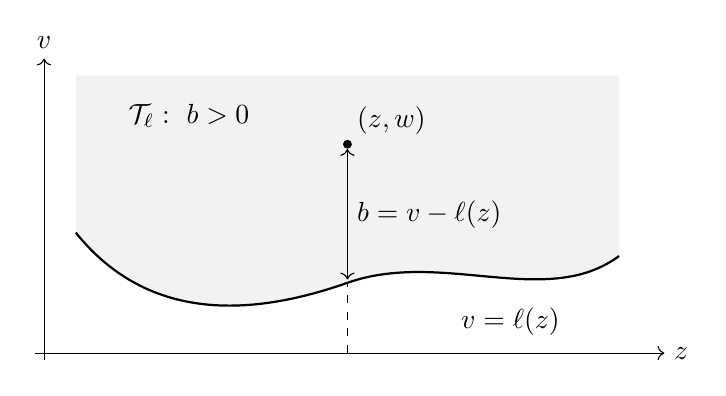
\begin{tikzpicture}[x=1.15cm,y=.85cm]
 \fill[black!5]
  (-3,1.8) .. controls (-2.2,.45) and (-1.05,.55) .. (0,1.05)
  .. controls (1.05,1.55) and (2.2,.65) .. (3,1.45)
  -- (3,4.15) -- (-3,4.15) -- cycle;
 \draw[->] (-3.45,0) -- (3.5,0) node[right] {$z$};
 \draw[->] (-3.35,-.1) -- (-3.35,4.4) node[above] {$v$};
 \draw[thick]
  (-3,1.8) .. controls (-2.2,.45) and (-1.05,.55) .. (0,1.05)
  .. controls (1.05,1.55) and (2.2,.65) .. (3,1.45);
 \node[anchor=north] at (1.8,.82) {$v=\ell(z)$};
 \draw[dashed] (0,0) -- (0,1.05);
 \draw[<->] (0,1.1) -- (0,3.05)
  node[midway,right] {$b=v-\ell(z)$};
 \fill (0,3.12) circle (1.6pt);
 \node[above right] at (0,3.12) {$(z,w)$};
 \node at (-1.75,3.55) {$\mathcal T_\ell:\ b>0$};
\end{tikzpicture}

 \caption{A schematic real slice of the tube.  The coordinate
 $b=v-\ell(z)$ is the positive vertical gap; $u$ and the other base
 directions are suppressed.  No convexity of the graph is assumed.}
 \label{tube:geometry}
\end{figure}

\emph{Completeness.}
Let $\gamma$ be a locally piecewise smooth curve of finite
$g_{\mathcal T}$-length, with its parameter tending to an endpoint.
Equation~\eqref{tube:real-decomposition} gives
\[
 \frac{|db(\dot\gamma)|}{2b}\le |\dot\gamma|_{g_{\mathcal T}}.
\]
Thus $\log b$ has finite total variation.  In particular, along this
curve there are constants $0<b_-\le b\le b_+<\infty$, and $b$ has a
positive limit.  The same metric identity implies
\[
 |(\pi\circ\gamma)'|_{g_\ell}
 \le \sqrt{b_+}\,|\dot\gamma|_{g_{\mathcal T}}.
\]
The base projection therefore has finite length and converges by
completeness of $g_\ell$.  Its image has compact closure.  On that
compact set $|d^c\ell|_{g_\ell}$ is bounded by some constant $C$, so
\[
 |u'|
 \le |(du+d^c\ell)(\dot\gamma)|
       +|d^c\ell((\pi\circ\gamma)')|
 \le 2b_+|\dot\gamma|_{g_{\mathcal T}}
       +C|(\pi\circ\gamma)'|_{g_\ell}.
\]
Hence $u$ also converges.  Since $v=b+\ell(z)$, the curve has a limit
in $\mathcal T_\ell$.  This finite-length criterion proves metric
completeness.  Indeed, a Cauchy sequence without a limit would have a
subsequence whose successive distances are less than $2^{-j}$;
joining successive points by paths of length less than $2^{1-j}$
would produce a finite-length curve without a limit.

\emph{The curvature comparison.}
For a Hermitian matrix $g=(g_{a\bar b})$ arising from a K\"ahler
potential, denote its Hermitian curvature components by
\begin{equation}\label{tube:hermitian-curvature}
 \mathcal R^g_{a\bar b c\bar d}
 =-\partial_a\partial_{\bar b}g_{c\bar d}
   +\sum_{p,q}g^{p\bar q}
       (\partial_a g_{c\bar q})(\partial_{\bar b}g_{p\bar d}).
\end{equation}
We record explicitly how these components determine the real
sectional numerator in our normalization.  If
$\xi^a=dz^a(X)$ and $\eta^a=dz^a(Y)$, set
\[
 T^{a\bar b}=i(\xi^a\bar\eta^b-\eta^a\bar\xi^b).
\]
Expansion of $X=\sum_a(\xi^a\partial_{z^a}
+\bar\xi^a\partial_{\bar z^a})$ and similarly of $Y$, using the
K\"ahler curvature symmetries, gives
\begin{align}
 R_g(X,Y,Y,X)
 &=\mathcal R^g(\xi,\bar\xi,\eta,\bar\eta)
   -\operatorname{Re}\mathcal R^g(\xi,\bar\eta,\xi,\bar\eta)
       \label{tube:real-complex-curvature}\\
 &=\frac12\sum_{a,b,c,d}
        \mathcal R^g_{a\bar b c\bar d}
        T^{a\bar b}T^{c\bar d}.\nonumber
\end{align}
The factor $1/2$ reflects that the complexification of the real
metric satisfies
$g(\partial_{z^a},\partial_{\bar z^b})=g_{a\bar b}/2$.

Fix a point of the tube over a base point $z_0$.  Choose holomorphic
K\"ahler normal coordinates on the base, centered at $z_0$, so that
$(\ell_{a\bar b})$ is the identity and its first derivatives vanish
there.  Such coordinates follow by a linear normalization followed
by a quadratic holomorphic change of coordinates; the K\"ahler
symmetry makes the quadratic coefficients symmetric in their two
holomorphic indices.  The mixed terms of total degree three in the
potential then vanish.  Subtracting the real part of a holomorphic
polynomial of degree at most three removes its remaining nonconstant
pure terms.  This subtraction is absorbed by a holomorphic
translation of $w$: if $\ell=\ell_0+\operatorname{Re}H$, replace
$w$ by $w-iH$.  Thus in the adapted coordinates the base potential
has three-jet
\[
 c+|z|^2.
\]

Compare the tube potential at this point with
\begin{equation}\label{tube:model-potential}
 \Phi_0=-\log(\operatorname{Im}w-c-|z|^2).
\end{equation}
The two metrics and their first derivatives agree at the point.
Their cubic contractions in
Equation~\eqref{tube:hermitian-curvature} therefore agree.  In the
fourth potential derivatives the only difference is the term
$b^{-1}\ell_{a\bar b c\bar d}$ with all four indices in the base.
The base cubic contractions vanish in the normal coordinates, so
\begin{equation}\label{tube:hermitian-transfer}
 \mathcal R^{g_{\mathcal T}}-\mathcal R^{g_{\Phi_0}}
 =b^{-1}\pi^*\mathcal R^{g_\ell}
 \qquad\text{at the comparison point}.
\end{equation}
Applying Equation~\eqref{tube:real-complex-curvature} gives the
corresponding identity of real sectional numerators:
\begin{equation}\label{tube:real-transfer}
 \begin{split}
 R_{g_{\mathcal T}}(X,Y,Y,X)
 &=R_{g_{\Phi_0}}(X,Y,Y,X)\\
 &\quad+b^{-1}R_{g_\ell}(d\pi X,d\pi Y,d\pi Y,d\pi X).
 \end{split}
\end{equation}
In particular, the extra term is nonpositive for every real pair
$X,Y$.  This remains true when their base projections are linearly
dependent, in which case that term is zero.  The comparison metrics
agree at the point, so the sectional-curvature denominators also
agree.

\emph{The model normalization.}
Put $\widetilde w=w-ic$.  The Cayley coordinates
\[
 (\mathcal Z,\mathcal W)
 =\left(\frac{2z}{\widetilde w+i},
         \frac{\widetilde w-i}{\widetilde w+i}\right)
\]
satisfy
\[
 1-|\mathcal Z|^2-|\mathcal W|^2
 =\frac{4(\operatorname{Im}\widetilde w-|z|^2)}
        {|\widetilde w+i|^2}.
\]
Consequently the potential in Equation~\eqref{tube:model-potential}
equals $-\log(1-|\mathcal Z|^2-|\mathcal W|^2)$ up to a
pluriharmonic summand and a constant.  Our comparison point has
$z=0$.  A real translation of $\widetilde w$ and a dilation
$(z,\widetilde w)\mapsto(z/\sqrt r,\widetilde w/r)$, $r>0$, are
model isometries and place it at $(0,i)$, which the Cayley map sends
to the ball origin.

Writing $Z$ for all the ball coordinates, expansion of
$-\log(1-|Z|^2)$ at zero gives
\[
 g_{a\bar b}(0)=\delta_{ab},\qquad
 \partial g_{a\bar b}(0)=0,\qquad
 \mathcal R^{g_{\Phi_0}}_{a\bar b c\bar d}(0)
 =-(\delta_{ab}\delta_{cd}+\delta_{ad}\delta_{cb}).
\]
For real orthonormal $X,Y$ at the origin, their complex components
$\xi,\eta$ have norm one and satisfy
$\operatorname{Re}\langle\xi,\eta\rangle=0$.  Write
$\langle\xi,\eta\rangle=i\beta$, where $|\beta|\le1$.
Equation~\eqref{tube:real-complex-curvature} now gives
\begin{equation}\label{tube:model-sectional}
 \operatorname{Sec}_{g_{\Phi_0}}(X\wedge Y)
 =-1-3\beta^2\in[-4,-1].
\end{equation}
Combining Equations~\eqref{tube:real-transfer}
and~\eqref{tube:model-sectional} proves
$\operatorname{Sec}_{g_{\mathcal T}}\le-1$ on all real planes.
\end{proof}

The same comparison also explains why this construction need not
have a lower sectional-curvature bound.

\begin{corollary}\label{tube:negative-plane}
Under the hypotheses of Lemma~\ref{tube:transfer}, suppose that
$g_\ell$ has a real two-plane of strictly negative sectional
curvature at some point.  Then
\[
 \inf\operatorname{Sec}_{g_{\mathcal T}}=-\infty.
\]
\end{corollary}

\begin{proof}
Let $X,Y$ be an orthonormal basis of such a base plane $\sigma$.
At a point above it with height $b$, the distribution
\[
 \mathcal H=\ker db\cap\ker(du+d^c\ell)
\]
is $J$-invariant, and $d\pi$ identifies its metric with
$b^{-1}g_\ell$.  If $\widehat X,\widehat Y$ are the horizontal lifts
of $X,Y$, then $\sqrt b\,\widehat X,\sqrt b\,\widehat Y$ are
$g_{\mathcal T}$-orthonormal.  Equation~\eqref{tube:real-transfer}
and the model computation give the exact formula
\[
 \operatorname{Sec}_{g_{\mathcal T}}
   (\widehat X\wedge\widehat Y)
 =-1-3g_\ell(JX,Y)^2+b\operatorname{Sec}_{g_\ell}(\sigma).
\]
Letting $b\to\infty$ proves the assertion.
\end{proof}

\section{Polynomial tests for bounded holomorphic functions}
\label{sec:analytic}

We will force the $w$-derivative of every bounded holomorphic function
$f$ on the tube to vanish. The elementary estimate comes from a holomorphic
disk through a point $(s_0,\zeta,w_0)$:
\[
 t\longmapsto(s_0,\zeta+t,w_0+i\alpha b t),\qquad |t|<L,
 \qquad \alpha,L>0,\quad |b|=1.
\]
If this disk lies in the tube and $|f|\le1$, Cauchy's inequality gives
\[
 |f_y(s_0,\zeta,w_0)+i\alpha b f_w(s_0,\zeta,w_0)|\le L^{-1}.
\]
We must prevent the two derivatives from canceling at many spatial
points. We arrange those points in root-of-unity cycles and hold $b$
constant on each cycle. A finite Fourier average then keeps only Taylor
degrees in one residue class. The phases will separate the prescribed
lowest-degree part of $f_w$ from the first few surviving terms of $f_y$,
with one phase choice valid for every polynomial of that degree.

The grids constructed below provide equidistributed projective directions
for polynomial sampling and cyclic affine lifts for this extraction.
Their additional separation and shell estimates will be used in
Section~\ref{sec:assembly} to localize the shear coefficients in disjoint
spatial neighborhoods when realizing the disks. After constructing the grids
and choosing the phases, we formulate the precise disk conditions and
prove that repeated tests force the holomorphic Liouville property.

Throughout this section, $\sigma$ denotes the unitary-invariant
probability measure on $\mathbb P^{n-1}$.  All norms on vectors and
derivatives are Euclidean unless indicated otherwise.  Constants may
depend on the fixed dimension $n$; the exponents in the separation
estimate below do not.

\subsection{Polynomial grids and their affine lifts}

\begin{lemma}[Homogeneous polynomial grids]
\label{grid:polynomials}
Fix $n\ge2$.  For every sufficiently large integer $N$ one can choose a
system of homogeneous polynomials of degree $N$,
\[
 Q_N=(H_N,p_N):\mathbb C^n\longrightarrow\mathbb C^{n-1}\times\mathbb C,
\]
with the following properties.  These choices can be made along all
integers $N\to\infty$, or along any prescribed sequence of degrees
tending to infinity.
\begin{enumerate}
\item There is a constant $C_n$ such that
\begin{equation}
 \label{grid:sphere-bounds}
 N^{-C_n}\le |Q_N(u)|\le N\qquad (|u|=1).
\end{equation}
\item The projective zero set of $H_N$ consists of
$M_N=N^{n-1}$ transverse points.  A subset $\mathcal G_N$ of these
points satisfies
\[
 |\mathcal G_N|=(1-o(1))M_N,
 \qquad
 \frac1{M_N}\sum_{\xi\in\mathcal G_N}\delta_\xi
 \ \rightharpoonup\ \sigma.
\]
For every $\xi\in\mathcal G_N$ and every unit representative $u$ of
$\xi$,
\begin{equation}
 \label{grid:goodness}
 N^{-1}\le |p_N(u)|\le N,
 \qquad
 \operatorname{sing}_{\min}
       \bigl(DH_N(u)|_{u^\perp}\bigr)\ge N^{-1}.
\end{equation}
\item Above each $\xi\in\mathcal G_N$, choose any lift $v_\xi$ such
that $p_N(v_\xi)=1$.  All $N$ lifts
\[
 e^{2\pi i q/N}v_\xi,\qquad 0\le q<N,
\]
have radii in $[N^{-1/N},N^{1/N}]$.  With the absolute choice
$k_*=30$, the Euclidean balls of radius $2N^{-k_*}$ about all these
lifts are pairwise disjoint.  If $v$ is one of the lifts, then
\begin{equation}
 \label{grid:shell-bound}
 |(H_N(z),p_N(z)-1)|\ge N^{-k_*-10}
 \quad\hbox{when}\quad
 N^{-k_*}\le |z-v|\le2N^{-k_*}.
\end{equation}
In a neighborhood of radius $4N^{-k_*}$ of every such lift, the first
and second derivatives of $Q_N$ have norm $O_n(N^5)$.
\end{enumerate}
In particular, weak approximation to any prescribed finite collection
of continuous test functions, with any fixed positive accuracy, can be
required by taking $N$ sufficiently large.
\end{lemma}

\begin{proof}
We use the standard unitary-invariant Gaussian ensemble of homogeneous
polynomials; its covariance and conditional zero-density framework appear
in \citet[Sections~2.2 and~2.4]{BleherShiffmanZelditch2000}. The proof
below supplies the needed formulas and all additional quantitative grid
properties. Randomness is used only to establish existence. A
standard circular complex Gaussian has density
$\pi^{-1}e^{-|z|^2}$ on $\mathbb C$.  Choose the components of $Q_N$
independently, with
\[
 Q_N^{(a)}(z)=
 \sum_{|\beta|=N}\left(\frac{N!}{\beta!}\right)^{1/2}
       g_{a,\beta}z^\beta,
 \qquad
 \mathbb E\bigl[Q_N^{(a)}(z)
       \overline{Q_N^{(a)}(u)}\bigr]=(z\cdot\bar u)^N.
\]
Here all $g_{a,\beta}$ are independent standard circular complex
Gaussians.  The covariance identity is the multinomial formula.  In
particular, at a unit vector the components of $Q_N$ are independent
standard complex Gaussians, and the law is invariant under unitary
changes of coordinates.

We first prove \eqref{grid:sphere-bounds} with probability tending to
one.  If $A=\sup_{|z|=1}|Q_N(z)|$, homogeneity gives
$\sup_{|z|\le1+1/N}|Q_N(z)|\le eA$.  Cauchy's inequality on complex
lines therefore bounds the first derivative on the unit sphere by
$CNA$, with an absolute constant $C$.  A sphere net of mesh $c/N$,
with a sufficiently small absolute $c$, consequently contains a point
where the norm is at least $A/2$.  Such a net has
$O_n(N^{2n-1})$ points.  Gaussian tails show
\[
 \mathbb P(A>N)\le C_n' N^{2n-1}e^{-c_n' N^2}\longrightarrow0.
\]
On the event $A\le N$, the Lipschitz constant on the sphere is at
most $CN^2$.  Use a second net of mesh $cN^{-C_n-2}$.  If the norm
somewhere on the sphere is less than $N^{-C_n}$, it is less than
$2N^{-C_n}$ at a point of this net.  A standard complex Gaussian
vector in $\mathbb C^n$ has probability at most $C_n' r^{2n}$ of
lying in a ball of radius $r$.  The union bound is therefore at most
\[
 C_n' N^{(C_n+2)(2n-1)-2nC_n}
   =C_n' N^{-C_n+4n-2}.
\]
Choose, for example, $C_n=8n$.  This proves both sphere bounds with
probability tending to one.

Put $d=n-1$.  Almost surely the projective zeros of the $d$-component
system $H_N$ are transverse.  To see this directly, let $\mathcal A$
be its finite-dimensional complex coefficient space.  Evaluation at
any point of $\mathbb P^d$ maps $\mathcal A$ onto the fiber of
$\mathcal O(N)^{\oplus d}$.  Hence the universal zero incidence
manifold is smooth, and a coefficient vector is a regular value of its
projection to $\mathcal A$ precisely when the corresponding section
has only transverse zeros.  Sard's theorem gives a Lebesgue-null
exceptional set; the Gaussian law is absolutely continuous.
Transversality and compactness imply that the zero set is finite.
The projective B\'ezout theorem for a zero-dimensional intersection of
$d$ hypersurfaces of degrees $N,\ldots,N$ gives total intersection
number $N^d$; every transverse intersection has multiplicity one
\citep[Theorem~III-71]{EisenbudHarris2000GeometrySchemes}.  Thus the number of zeros is the deterministic
quantity $M_N=N^d$ almost surely.

We next justify the counting formulas needed for equidistribution.
They are the one- and two-point, zero-dimensional cases of the
correlation formula in \citet[Theorem~2.1]{BleherShiffmanZelditch2000}.
Our subsequent off-diagonal argument proves the particular convergence
needed here; the more general simultaneous-zero convergence theorem of
\citet[Corollary~1.3]{Shiffman2008Convergence} supplies a broader context.
In a holomorphic coordinate chart of $\mathbb P^d$, regard the system
as a holomorphic map $H_a(z)$ depending linearly on its coefficients.
Locally split those coefficients as $(a,b)$ so that
\[
 H_{a,b}(z)=E(z)a+R(z,b),\qquad \det E(z)\ne0.
\]
This is possible because evaluation is surjective.  The equation
$H_{a,b}(z)=0$ is equivalent to
$a=A(z,b):=-E(z)^{-1}R(z,b)$.  At a zero, with
$J=D_zH_{a,b}(z)$,
\[
 D_zA=-E(z)^{-1}J.
\]
For fixed $b$, the change-of-variables formula with multiplicity for
$z\mapsto A(z,b)$ thus introduces the real Jacobian
$|\det E|^{-2}|\det J|^2$.  Integrating in $b$ against the smooth
Gaussian coefficient density yields the one-point zero density
\begin{equation}
 \label{grid:one-point-density}
 \rho_{1,N}(z)=
 p_{H_N(z)}(0)\,
 \mathbb E\bigl[|\det DH_N(z)|^2\mid H_N(z)=0\bigr].
\end{equation}
The same argument works with a bounded measurable mark multiplying
the zero count.  It first applies to nonnegative marks, and the
general bounded case follows by decomposition.

For two distinct projective points, joint evaluation onto the two
fibers is surjective.  Indeed, powers of linear forms that vanish at
one point and not the other give independent prescribed values for
each component.  Solve now for $2d$ coefficient variables and apply
the same change of variables in the two point coordinates.  The
point Jacobian is block diagonal, giving
\begin{equation}
 \label{grid:two-point-density}
 \begin{split}
 \rho_{2,N}(z,z')={}&p_{(H_N(z),H_N(z'))}(0,0)\\
 &\quad\cdot
 \mathbb E\bigl[
   |\det DH_N(z)|^2|\det DH_N(z')|^2
       \mid H_N(z)=H_N(z')=0\bigr].
 \end{split}
\end{equation}
Partitions of unity give these formulas on projective space and on
the complement of its diagonal, respectively.  This derivation uses
only the coefficient density and ordinary change of variables; no
independence of zeros has been assumed.

At a point represented by a unit vector $u$, take affine tangent
coordinates $u+\sum_{j=1}^d z_j e_j$ with $(e_j)$ orthonormal in
$u^\perp$.  Differentiating the covariance shows that $H_N(u)$ is
independent of $N^{-1/2}DH_N(u)|_{u^\perp}$, and that the latter is
a $d\times d$ matrix of independent standard complex Gaussians.
At two distinct projective points, the cross-covariances of these
normalized value and first-derivative data tend to zero locally
uniformly off the diagonal.  More explicitly, on a compact set of
pairs with $|u\cdot\bar v|\le\rho<1$, they are bounded by a fixed
power of $N$ times $\rho^{N-2}$.  This follows by differentiating
$(u\cdot\bar v)^N$ at most once at each point.  The joint Gaussian
covariance consequently converges uniformly there to the direct sum
of its one-point covariances.  Conditional Gaussian covariances given
the values zero converge as well.  Gaussian moments of the fixed
polynomials $|\det J|^2$ and their products therefore converge.
Equations \eqref{grid:one-point-density} and
\eqref{grid:two-point-density} imply that the two-point density,
divided by $M_N^2$, converges locally uniformly off the diagonal to
the product of the normalized one-point densities.

The exact total number of zeros lets us pass from off-diagonal
decorrelation to weak convergence without estimating the two-point
density near the diagonal. Let
\[
 \mu_N=\frac1{M_N}\sum_{H_N(\xi)=0}\delta_\xi.
\]
Unitary invariance and the deterministic count imply
$\mathbb E\mu_N=\sigma$.  The positive measure
$\mathbb E(\mu_N\otimes\mu_N)$ has total mass one.  Off the
diagonal, its density converges to that of $\sigma\otimes\sigma$,
by the preceding calculation.  This implies convergence on the
whole product: given $\varepsilon>0$, choose a compact subset of the
off-diagonal region having $(\sigma\otimes\sigma)$-mass greater
than $1-\varepsilon$.  Its mass under
$\mathbb E(\mu_N\otimes\mu_N)$ is greater than $1-2\varepsilon$
for all sufficiently large $N$.  At most $2\varepsilon$ of the
total mass can remain elsewhere.  Since the diagonal has zero
$(\sigma\otimes\sigma)$-mass, there is no additional limiting
mass there.  Thus
\[
 \mathbb E(\mu_N\otimes\mu_N)
       \rightharpoonup\sigma\otimes\sigma.
\]
For every continuous test function, its integral against $\mu_N$
therefore has variance tending to zero.  This proves weak
convergence to $\sigma$ in probability.

It remains to discard the bad zeros.  Use
\eqref{grid:one-point-density} with marks.  If $G$ is a $d\times d$
standard complex Gaussian matrix, then at a zero the derivative
condition in \eqref{grid:goodness} fails only when
$\operatorname{sing}_{\min}(G)<N^{-3/2}$.  Its expected discarded
fraction is
\[
 \frac{\mathbb E\bigl[
       |\det G|^2
       \boldsymbol{1}_{\{\operatorname{sing}_{\min}(G)<N^{-3/2}\}}
       \bigr]}{\mathbb E|\det G|^2}
       \longrightarrow0.
\]
Indeed a Gaussian square matrix is nonsingular almost surely,
$|\det G|^2$ is integrable, and dominated convergence applies.
The independent polynomial $p_N$ has a standard complex Gaussian
value at every unit representative.  Its two forbidden tails have
probability
\[
 \mathbb P(|p_N|<N^{-1})+\mathbb P(|p_N|>N)
   =1-e^{-N^{-2}}+e^{-N^2}\longrightarrow0.
\]
Markov's inequality shows that the total discarded fraction tends
to zero in probability.  Removing that fraction does not alter weak
convergence.  The modulus and singular-value conditions are
unchanged on multiplying a unit representative by a phase, so they
hold for every such representative.

We may now select deterministic systems.  Take a countable uniformly
dense family of continuous functions on projective space, and impose
successively accurate conditions on successively longer finite
subfamilies.  Convergence in probability, the vanishing bad
fraction, and the probability-one transversality statement show that
these conditions and \eqref{grid:sphere-bounds} have a nonempty
intersection for every sufficiently large degree.  Choose one system
from that intersection.  A diagonal choice gives all the asserted
limits and works equally well along any prescribed sequence of
degrees.

We have obtained the projective sampling properties. It remains to
provide disjoint neighborhoods in which Section~\ref{sec:assembly} can
localize its shear coefficients. Fix a good direction and a lift
$v$ with $p_N(v)=1$.
Homogeneity and \eqref{grid:goodness} give
$N^{-1/N}\le |v|\le N^{1/N}$.  In the splitting of the domain into
the radial complex line and its Hermitian orthogonal complement,
$DH_N(v)$ vanishes on the radial line, while
$Dp_N(v)$ has radial derivative $N/|v|$.  The transverse derivative
of $H_N$ has least singular value at least $N^{-4}$ for large $N$:
the scaling from a unit representative costs at most one additional
factor $N$, so this is a deliberately weaker bound than necessary.
Homogeneity, the sphere upper bound, and Cauchy's inequality at
scale $c/N$ give first- and second-derivative bounds $O_n(N^5)$ in
the stated neighborhood.  At the lift itself, the transverse first
derivatives are $O_n(N^4)$.  Block inversion therefore gives
\[
 \bigl\|D(H_N,p_N-1)(v)^{-1}\bigr\|\le N^9
\]
for all sufficiently large $N$.  Taylor's formula, uniformly for
$|z-v|\le4N^{-30}$, now yields
\[
 |(H_N(z),p_N(z)-1)|
 \ge N^{-9}|z-v|-C_n' N^5|z-v|^2
 \ge\tfrac12 N^{-9}|z-v|.
\]
This proves \eqref{grid:shell-bound}.  It also excludes every other
zero of $(H_N,p_N-1)$ within distance $4N^{-30}$, proving
disjointness of the balls about all good lifts.
\end{proof}

\subsection{Choosing phases uniformly for a fixed Taylor order}

The grids now supply many separated evaluation points. Their next role
is linear algebraic: we choose a phase at each projective point so that
no fixed-order polynomial jet can be hidden among the first few Taylor
degrees surviving a root-of-unity average. The independent-phase moment
calculation is the same quadratic-form identity used for random-phase
trace estimates in \citet{IitakaEbisuzaki2004}.
The additional rank and polynomial superlevel estimates give one phase
choice uniformly for an entire coefficient space.

\begin{lemma}[Phases separate low-degree jets]
\label{grid:phases}
Fix positive integers $k,n$, with $n\ge2$, such that
\begin{equation}
 \label{grid:dimension-choice}
 \sum_{j=1}^{k-1}\frac{j^{n-1}}{(n-1)!}<\frac1{100}.
\end{equation}
Fix a nonnegative integer $h$.  For sufficiently large polynomial
grids from Lemma~\ref{grid:polynomials}, choose one lift $v_\xi$
above each good direction and let $V_N\subset\mathbb C^{\mathcal G_N}$
be the space of evaluation vectors of sums of homogeneous
polynomials of degrees
\[
 h,\ h+N,\ \ldots,\ h+(k-1)N.
\]
Let $\Pi_N$ be orthogonal projection onto $V_N$ for the unweighted
Euclidean point norm.  There are phases $b_\xi$, $|b_\xi|=1$, and a
constant $\delta_h>0$, independent of $N$ and of the chosen lift
phases, such that
\begin{equation}
 \label{grid:phase-lower-bound}
 M_N^{-1/2}
 \left\|(1-\Pi_N)
       \bigl(b_\xi P(v_\xi)\bigr)_{\xi\in\mathcal G_N}\right\|
 \ge\delta_h\|P\|
\end{equation}
for every homogeneous polynomial $P$ of degree $h$.  Here $\|P\|$
is any fixed Euclidean norm on its coefficient space, chosen
independently of the grid.  All required grid accuracies and degree
thresholds depend only on the fixed $n,k,h$ and this norm.
\end{lemma}

\begin{proof}
Dimension gives
\[
 \frac{\operatorname{rank}\Pi_N}{M_N}
 \le N^{1-n}\sum_{j=0}^{k-1}
       \binom{h+jN+n-1}{n-1}<\frac2{100}
\]
for all sufficiently large $N$.  Indeed its limit is the sum in
\eqref{grid:dimension-choice}.

There is a number $t_h>0$ such that, on every sufficiently accurate
grid, every polynomial with $\|P\|=1$ satisfies
\begin{equation}
 \label{grid:uniform-superlevel}
 |P(v_\xi)|>t_h
 \quad\hbox{at at least }0.8M_N\hbox{ good directions}.
\end{equation}
For completeness, a nonzero homogeneous polynomial has a
projective zero set of $\sigma$-measure zero.  In affine charts this
is the elementary fact that the zero set of a nonzero complex
polynomial has Lebesgue measure zero, obtained by induction and
Fubini's theorem.  Thus, for each norm-one polynomial $P$, some
positive threshold has a superlevel set of measure greater than
$0.9$.  Uniform continuity in the coefficients makes the same
superlevel estimate, with a smaller threshold, valid in a
neighborhood of $P$.  The coefficient unit sphere is compact, so
finitely many such neighborhoods suffice and their thresholds have
a positive common lower bound.  Weak convergence of the grid
measures applied to these finitely many open superlevel sets gives
the estimate for unit representatives, with a fixed margin in both
threshold and counting proportion.  Since
$|v_\xi|^h\to1$ uniformly, it gives
\eqref{grid:uniform-superlevel}.  This proof requires only finitely
many fixed approximation conditions for the given $h$.

The projection has $0\le(\Pi_N)_{\xi\xi}\le1$ and diagonal sum
less than $0.02M_N$.  Consequently at most $0.04M_N$ diagonal
entries exceed $1/2$.  Choose the $b_\xi$ temporarily as independent
uniform phases.  Writing $Q_N'=1-\Pi_N$, independence gives
\[
 \begin{split}
 &\mathbb E\left[
 M_N^{-1}\left\|Q_N'
       \bigl(b_\xi P(v_\xi)\bigr)_\xi\right\|^2\right]\\
 &\hspace{25mm}=
 M_N^{-1}\sum_\xi
       \bigl(1-(\Pi_N)_{\xi\xi}\bigr)|P(v_\xi)|^2
 \ge0.38t_h^2
 \end{split}
\]
when $\|P\|=1$.  The last inequality uses the intersection of the
$0.8M_N$ indices in \eqref{grid:uniform-superlevel} with the
complement of the at most $0.04M_N$ high-leverage indices.

We need a single phase choice for all polynomials, rather than a
choice depending on $P$.  Let $(e_a)$ be a fixed orthonormal basis
of the degree-$h$ coefficient space, and put $q_a(\xi)=e_a(v_\xi)$.
These evaluations have a common bound depending only on $n,h$ and
the chosen norm.  The Gram matrix of the random linear map in
\eqref{grid:phase-lower-bound} has entries
\[
 G_{ab}=M_N^{-1}\sum_{\xi,\eta}
       \overline{q_a(\xi)}\,\overline{b_\xi}
       (Q_N')_{\xi\eta}b_\eta q_b(\eta).
\]
Its diagonal-index terms are deterministic.  For distinct indices,
the products $\overline{b_\xi}b_\eta$ are orthonormal in
$L^2$ of the phase probability space: two such ordered products
have nonzero inner product only when their ordered pairs agree.
In particular, reversal of the pair gives expectation
$\mathbb E(\overline{b_\xi}^{\,2}b_\eta^2)=0$.
It follows that
\[
 \begin{split}
 \mathbb E|G_{ab}-\mathbb EG_{ab}|^2
 &\le C_{n,h}M_N^{-2}
       \sum_{\xi\ne\eta}|(\Pi_N)_{\xi\eta}|^2\\
 &\le C_{n,h}M_N^{-2}\operatorname{rank}\Pi_N
   =O_{n,h}(M_N^{-1}).
 \end{split}
\]
The Gram matrix has fixed finite size.  Chebyshev's inequality
therefore implies that its operator-norm distance from its mean
tends to zero in probability.  Its mean is bounded below by
$0.38t_h^2$ times the identity.  A phase choice with least
eigenvalue at least $0.19t_h^2$ exists for every sufficiently large
grid.  Taking $\delta_h=\sqrt{0.19}\,t_h$ proves the assertion.
All estimates used only absolute values of lift evaluations, so
the threshold and lower bound are uniform over their arbitrary
representative phases.
\end{proof}

\begin{remark}
\label{grid:finite-dimension}
For every fixed $k$, condition \eqref{grid:dimension-choice} holds
in some sufficiently large finite dimension.  Indeed, with
$r=n-1$, its left side is bounded by
$(k-1)^{r+1}/r!$, which tends to zero as $r\to\infty$.
The argument will use one such fixed dimension, not an assertion
in every dimension.
\end{remark}

\subsection{From disk estimates to the holomorphic Liouville property}

\begin{lemma}[Root-of-unity extraction]
\label{grid:frequency}
Let $0\le h<N$, and suppose $g$ is holomorphic on a neighborhood of
the closed ball $|s|\le S$, with $|g|\le K$ there.  Write
$g=\sum_{r\ge0}g_r$ for its homogeneous Taylor expansion at zero.
If $R|v|<S$, then
\[
 \frac1N\sum_{q=0}^{N-1}e^{-2\pi i hq/N}
       g(Re^{2\pi i q/N}v)
   =\sum_{j\ge0}g_{h+jN}(Rv).
\]
If $R|v|/S\le e^{-0.99c/N}$ and $c\ge1$, truncating the sum after
$j=k-1$ has error at most $C K e^{-0.99kc}$, while retaining just
the term $g_h(Rv)$ has error at most $C K e^{-0.99c}$.  The constant
$C$ is absolute, independent of $N,h,R,S$.
\end{lemma}

\begin{proof}
Cauchy's inequality on the complex line through $v$ gives
\[
 |g_r(Rv)|\le K(R|v|/S)^r.
\]
The homogeneous expansion converges absolutely at the evaluation
points.  The finite Fourier average annihilates every degree not
congruent to $h$ modulo $N$, giving the identity.  Put
$\theta=R|v|/S$.  The first tail is bounded by
\[
 K\sum_{j=k}^{\infty}\theta^{h+jN}
   \le\frac{K e^{-0.99kc}}{1-e^{-0.99c}}.
\]
The case $k=1$ gives the other estimate.  The denominator is
bounded away from zero for $c\ge1$.
\end{proof}

We now convert these finite-dimensional estimates into the analytic
condition needed by the geometric construction. A large sheared disk
bounds a linear combination of the $y$- and $w$-derivatives. The phases
separate the degree-$h$ part of the latter from the former. Heights
$D_j$ growing more slowly than the accuracy parameters $c_j$ will let
the three-lines theorem turn smallness at those heights into vanishing.

\begin{proposition}[A testing criterion for the holomorphic Liouville property]
\label{grid:criterion}
Fix constants $p_0,p_1\ge0$ and $m_0>p_1$.  Choose an integer $k$
and a finite dimension $n\ge2$ so that
\begin{equation}
 \label{grid:exponent-choice}
 0.99k>p_0+p_1+1,
 \qquad
 \sum_{r=1}^{k-1}\frac{r^{n-1}}{(n-1)!}<0.01.
\end{equation}
Let $(\zeta_j,h_j)$ be a sequence of pairs from a countable dense
subset of an open disk in $\mathbb C$ and the nonnegative integers,
with every pair repeated infinitely often.  At stage $j$, choose
numbers $R_j\ge1$, $c_j\ge1$, an integer $N_j>h_j$, and a grid
from Lemma~\ref{grid:polynomials} sufficiently large and accurate
for Lemma~\ref{grid:phases} at order $h_j$.  Set
\[
 S_j=R_j e^{c_j/N_j},\qquad \log N_j\le c_j/100.
\]
Choose heights $D_j$ and positive numbers $\alpha_j$ such that
\[
 \alpha_j^{-1}\le e^{p_1c_j},
\]
and, along the repetitions of every fixed pair,
\begin{equation}
 \label{grid:height-rates}
 c_j\longrightarrow\infty,\qquad
 D_j\longrightarrow\infty,\qquad
 \frac{D_j}{c_j}\longrightarrow0.
\end{equation}
There are phases $b_{j,\xi}$, one per good projective direction
and constant throughout its cycle of lifts, with the following
property.

Let $\ell$ be a smooth real function on $\mathbb C^n\times\mathbb C$,
and let
\[
 \mathcal T=\{(s,y,w):\operatorname{Im}w>\ell(s,y)\}.
\]
Suppose every stage satisfies these conditions:
\begin{enumerate}
\item On $|s|\le S_j$,
\begin{equation}
 \label{grid:height-gap}
 \ell(s,\zeta_j)\le D_j-2.
\end{equation}
\item For every holomorphic $f$ on $\mathcal T$ with $|f|\le1$,
every $w$ with $\operatorname{Im}w=D_j$, and every $|s|=S_j$,
\begin{equation}
 \label{grid:sphere-derivative}
 |f_y(s,\zeta_j,w)|\le e^{p_0c_j}.
\end{equation}
\item For every good direction $\xi$, every lift
$v=e^{2\pi iq/N_j}v_\xi$, and every $w$ on that height line, the
holomorphic disk
\begin{equation}
 \label{grid:sheared-disk}
 t\longmapsto
 \bigl(R_jv,\ \zeta_j+t,\ w+i\alpha_j b_{j,\xi}t\bigr),
 \qquad |t|<e^{m_0c_j},
\end{equation}
is contained in $\mathcal T$.
\end{enumerate}
Then every bounded holomorphic function on $\mathcal T$ is constant.
The phases depend only on the grids and their assigned jet orders,
not on $\ell$, $f$, or $w$.
\end{proposition}

\begin{proof}
For each stage choose the phases supplied by
Lemma~\ref{grid:phases}.  Assign its phase to all $N_j$ lifts of
the same direction.  We prove the assertion for a holomorphic
function with $|f|\le1$, which suffices by constant rescaling.

Fix a stage and temporarily omit its subscript.  For each $w$ with
$\operatorname{Im}w=D$, put
\[
 A(s)=f_y(s,\zeta,w),\qquad I(s)=i f_w(s,\zeta,w).
\]
Both are holomorphic on a neighborhood of the closed spatial ball
$|s|\le S$, by the strict height margin and compactness.  The
maximum principle and \eqref{grid:sphere-derivative} give
$|A|\le e^{p_0c}$ on the ball.  The unit $w$-disk centered at any
$(s,\zeta,w)$ in this ball lies in $\mathcal T$, by
\eqref{grid:height-gap}; Cauchy's inequality gives $|I|\le1$.
On a sheared disk, the derivative at $t=0$ is
$A(Rv)+\alpha b_\xi I(Rv)$.  Thus
\begin{equation}
 \label{grid:node-inequality}
 |A(Rv)+\alpha b_\xi I(Rv)|\le e^{-m_0c}.
\end{equation}
Every estimate so far is uniform in the real part of $w$.

For each good direction take the Fourier average in
Lemma~\ref{grid:frequency} over its cycle.  Since $b_\xi$ is
constant on that cycle, it factors out of the averaged second
term of \eqref{grid:node-inequality}.  The lift radius bound gives
\[
 \frac{R|v_\xi|}{S}
 \le\exp\left(\frac{\log N-c}{N}\right)
 \le e^{-0.99c/N}.
\]
Let $a$ and $i'$ be the resulting vectors of averaged $A$ and $I$
values, respectively.  There is a vector $a_0\in V_N$ such that
\[
 \|a-a_0\|_\infty\le C e^{(p_0-0.99k)c}.
\]
If $P$ is the homogeneous degree-$h$ Taylor term of the function
$s\mapsto I(Rs)$, then
\[
 \bigl\|i'-(P(v_\xi))_\xi\bigr\|_\infty
       \le C e^{-0.99c}.
\]
The averaged node inequalities still have supremum norm at most
$e^{-m_0c}$.  Apply $1-\Pi_N$ and use $a_0\in V_N$.  Since the
number of good directions is at most $M_N$, conversion from the
supremum norm to $M_N^{-1/2}$ times Euclidean norm costs at most
one.  Lemma~\ref{grid:phases} consequently gives
\[
 \begin{split}
 \alpha\delta_h\|P\|
 &\le e^{-m_0c}
       +C e^{(p_0-0.99k)c}
       +C\alpha e^{-0.99c},\\
 \|P\|
 &\le C_h\left(
       e^{(p_1-m_0)c}
       +e^{(p_1+p_0-0.99k)c}
       +e^{-0.99c}\right).
 \end{split}
\]
In particular, with the fixed positive number
\[
 \varepsilon=\min\{m_0-p_1,\ 0.99k-p_0-p_1,\ 0.99\},
\]
we have
\begin{equation}
 \label{grid:jet-decay}
 \|P\|\le C_h e^{-\varepsilon c}.
\end{equation}
The constants are independent of the stage once $h$ is fixed.
This is exactly the uniformity in Lemma~\ref{grid:phases}; the
Fourier tail denominator is $1-e^{-0.99c}$, not
$1-e^{-0.99c/N}$.  Since every degree-$h$ coefficient of $I(Rs)$
is $R^h$ times the corresponding coefficient of $I(s)$ and
$R\ge1$, \eqref{grid:jet-decay} bounds each degree-$h$ coefficient
of $f_w(s,\zeta,w)$ by the same exponential rate.

We have obtained exponential decay for every coefficient of the
prescribed degree, uniformly along the entire horizontal $w$-line.
It remains to bring that estimate down from the growing testing heights
to a fixed open part of the tube.

Fix now a scheduled center $\zeta$ and a multiindex $\beta$ of
length $h$.  The coefficient
\[
 g_\beta(w)=\frac1{\beta!}
       \partial_s^\beta f_w(0,\zeta,w)
\]
is holomorphic on the whole connected half-plane
$\operatorname{Im}w>\ell(0,\zeta)$.  At every point of this
half-plane a spatial neighborhood is available, so the derivative
is well-defined and holomorphic there.  Choose once a small
closed spatial polydisk about zero and a number $t_0$ exceeding
the supremum of $\ell(s,\zeta)$ on that polydisk by more than two.
Cauchy's inequalities in $s$ and on a unit $w$-disk give
\[
 |g_\beta(w)|\le B_\beta
 \qquad (\operatorname{Im}w\ge t_0),
\]
where $B_\beta$ is independent of every testing stage and of
$\operatorname{Re}w$.  Along the stages assigned to $(\zeta,h)$,
\eqref{grid:jet-decay} gives
\[
 \sup_{\operatorname{Im}w=D_j}|g_\beta(w)|
       \le C_h e^{-\varepsilon c_j}.
\]
For any fixed $t>t_0$, apply Hadamard's three-lines theorem
\cite[Theorem~7.13]{Tropp2022} to the horizontal strip between heights
$t_0$ and $D_j$, once $D_j>t$.
Writing $\theta_j=(t-t_0)/(D_j-t_0)$, it yields
\[
 \sup_{\operatorname{Im}w=t}|g_\beta(w)|
 \le B_\beta^{\,1-\theta_j}
       (C_h e^{-\varepsilon c_j})^{\theta_j}.
\]
If $B_\beta=0$ there is nothing to prove.  Otherwise, the
logarithm of the right side is
\[
 \log B_\beta+
 \frac{t-t_0}{D_j-t_0}
    \bigl(\log(C_h/B_\beta)-\varepsilon c_j\bigr)
       \longrightarrow-\infty
\]
by \eqref{grid:height-rates}.  Hence $g_\beta$ vanishes in the
upper half-plane and, by the identity theorem, throughout
$\operatorname{Im}w>\ell(0,\zeta)$.  Repeating this argument for
each order proves that all spatial Taylor coefficients of $f_w$
at zero vanish at every scheduled center.  Dependence of the
constants and of the preliminary height $t_0$ on the order causes
no difficulty: each order has its own infinite sequence, and
analytic continuation gives the same full half-plane afterwards.

To pass from these statements to a common open set, choose a
spatial ball about zero and an open subdisk of the center disk,
both with compact closures.  Choose $L$ larger than the supremum
of $\ell$ on their product.  On the product with
$\operatorname{Im}w>L$, the function $f_w$ is jointly holomorphic.
At each scheduled center in the subdisk, all of its spatial
Taylor coefficients vanish for every such $w$.  Taylor uniqueness
and the identity theorem on the spatial ball give vanishing on
that ball.  Continuity in $y$ and density of the scheduled centers
then give vanishing on the whole product.  The tube is connected:
the coordinates
\[
 (s,y,\operatorname{Re}w,
        \operatorname{Im}w-\ell(s,y))
\]
identify it with
$\mathbb C^{n+1}\times\mathbb R\times(0,\infty)$.
The several-variable identity theorem therefore gives $f_w=0$
everywhere on $\mathcal T$.

For every fixed $(s,y)$ the $w$-fiber is a connected half-plane,
so $f$ is constant along that fiber.  It descends to a bounded
function $F$ on $\mathbb C^{n+1}$.  This descended function is
holomorphic: near any base point choose a single constant $w_0$
whose imaginary part exceeds the supremum of $\ell$ on a small
base neighborhood, and write $F(s,y)=f(s,y,w_0)$ there.  These
local holomorphic definitions agree on overlaps by fiber
constancy.  Liouville's theorem, applied on complex lines in
$\mathbb C^{n+1}$, makes $F$, and therefore $f$, constant.
\end{proof}

\begin{remark}
\label{grid:geometric-interface}
Condition \eqref{grid:sphere-derivative} follows immediately if,
at the stated sphere points and heights, the unsheared $y$-disk
of radius $e^{-p_0c_j}$ lies in the tube.  Thus the criterion asks
the geometric construction for only three quantitative facts: a
height bound on a spatial ball, sufficiently wide unsheared disks
on its boundary, and much wider disks in the prescribed sheared
directions at its polynomial nodes.  The phase choices are made
before any bounded holomorphic function is considered.
\end{remark}

\section{The fiber Legendre transform and its curvature}\label{sec:fiber}

The analytic criterion leaves us a geometric task: construct the base
potential while retaining explicit curvature margins for later changes.
We first derive the metric and its six curvature blocks for a fixed fiber
center. The partial Legendre transform uses, up to our fixed metric
normalization, the fiber momentum of the circle-invariant constructions
of Calabi and Hwang--Singer \citep{Calabi1979,HwangSinger2002}.
We allow the radial profile to vary over the spatial base, which adds
spatial-derivative terms to the curvature. We compute the full tensor
before estimating these additional terms.

All spatial derivatives in this section are taken with the fiber momentum
\(\tau\) fixed, unless a different convention is stated explicitly.
The spatial variables are \(s=(s_1,\ldots,s_n)\), and the fiber variable is
\(y\in\mathbb C\).  Its center \(\zeta\) is constant in this section.
Let \(q(x,s)>0\), where \(x=\log\tau\), and choose \(F\) by
\begin{equation}\label{fiber:F}
 F_x=q^{-1},\qquad \lim_{x\to-\infty}(F(x,s)-x)=0.
\end{equation}
We assume that this normalization is possible, that \(F\to+\infty\)
as \(x\to+\infty\), and that \(q\), regarded as a function of \(\tau\),
is smooth at zero with \(q(0,s)=1\).  All these statements are local
uniformly in \(s\).  For smooth real functions \(B,\psi\), set
\begin{align}
 U(s,\tau)&=B(s)+\tau\psi(s)-\int_0^\tau F(\log v,s)\,dv,
 \label{fiber:U}\\
 \rho&=\log|y-\zeta|^2=F(\log\tau,s)-\psi(s),
 \label{fiber:inverse}\\
 \ell_{\mathrm{rad}}&=U+\tau\rho
 =B+\int_0^\tau q(\log v,s)^{-1}\,dv.
 \label{fiber:potential}
\end{align}
The last identity follows by integration by parts; the boundary term
\(vF(\log v,s)\) tends to zero as \(v\downarrow0\).
Since \(F_x>0\) and its endpoint limits are infinite with the indicated
signs, \eqref{fiber:inverse} determines a unique \(\tau>0\) for every
\(y\ne\zeta\).

Hereafter \(C=-R\) denotes the negative Hermitian curvature tensor:
\begin{equation}\label{fiber:curvature-convention}
 C_{\alpha\bar\beta\gamma\bar\delta}
 =\partial_\alpha\partial_{\bar\beta}g_{\gamma\bar\delta}
 -g^{\mu\bar\nu}
   (\partial_\alpha g_{\gamma\bar\nu})
   (\partial_{\bar\beta}g_{\mu\bar\delta}).
\end{equation}
The sectional-curvature sign associated with this convention is verified
below; in particular, positivity of the relevant contractions of \(C\)
means nonpositive Riemannian sectional curvature.

\begin{lemma}[Metric and regularity of the Legendre transform]
\label{fiber:metric}
Write
\[
 P=\tau q,\qquad V=(B_{i\bar j}),\qquad
 G=(\psi_{i\bar j}),\qquad h=(U_{i\bar j}),\qquad
 \mathcal N=h_\tau.
\]
Where \(h>0\), the complex Hessian of \(\ell_{\mathrm{rad}}\) is
\begin{equation}\label{fiber:metric-form}
 h_{i\bar j}\,ds_i\,d\bar s_j+
 P\left|d\log(y-\zeta)+U_{\tau i}\,ds_i\right|^2.
\end{equation}
It is positive off the axis.  Its spatial Schur complement is exactly
\(h\).  The potential and its complex Hessian extend smoothly across
\(y=\zeta\); on that axis the Hessian in the original splitting is
\(V\oplus e^\psi\), and is positive whenever \(V>0\).
\end{lemma}

\begin{proof}
Use the holomorphic coordinate \(z_0=\log(y-\zeta)\), so that
\(\rho=z_0+\bar z_0\).  Differentiating \(U_\tau+\rho=0\) gives
\[
 U_{\tau\tau}=-P^{-1},\qquad
 \partial_{z_0}\tau=P,\qquad
 \partial_{s_i}\tau=P U_{\tau i}.
\]
Differentiation of \(\ell=U+\tau\rho\) now gives
\[
 g_{0\bar0}=P,\qquad g_{i\bar0}=P U_{\tau i},\qquad
 g_{i\bar j}=h_{i\bar j}+P U_{\tau i}U_{\tau\bar j},
\]
which is \eqref{fiber:metric-form}.  For regularity, write
\(F=\log\tau+f(\tau,s)\).  The equation
\(f_\tau=(q^{-1}-1)/\tau\), with \(f(0,s)=0\), shows that \(f\)
is smooth.  Equation \eqref{fiber:inverse} becomes
\(\tau e^{f(\tau,s)}=e^\psi|y-\zeta|^2\).  Its derivative with respect
to \(\tau\) at zero is one, so the smooth implicit-function theorem
applies.  In particular,
\(\tau=e^\psi|y-\zeta|^2+O(|y-\zeta|^4)\).
Substitution in \eqref{fiber:potential} proves the stated extension and
axis metric.
\end{proof}

We use a local holomorphic change \(z_0\mapsto z_0+f(s)\) to make
\(U_{\tau i}=0\) at a specified point.  The corresponding change of
\(U\) is linear in \(\tau\) with a pluriharmonic spatial coefficient;
it leaves \(h\) and \(\mathcal N\) unchanged.  The quadratic jet of
\(f\) can also make \(U_{\tau ik}=0\) there.  We call these the tilted
logarithmic coordinates.  The coordinate changes used to evaluate a jet
are held fixed while that jet is differentiated.

\begin{lemma}[The six curvature blocks]\label{fiber:blocks}
In tilted logarithmic coordinates, the tensor
\eqref{fiber:curvature-convention} has the following blocks:
\begin{align}
 A:=C_{0\bar0 0\bar0}
   &=P^2P_{\tau\tau}-|\partial P|_h^2,
 \label{fiber:blockA}\\
 A_i:=C_{i\bar0 0\bar0}
   &=P\bigl(\partial_iP_\tau-
       (\mathcal N h^{-1}\partial P)_i\bigr),
 \label{fiber:blockAi}\\
 W_{i\bar j}:=C_{i\bar j0\bar0}
   &=P\bigl(\partial_i\partial_{\bar j}\log P
       +P_\tau\mathcal N_{i\bar j}
       -P(\mathcal N h^{-1}\mathcal N)_{i\bar j}\bigr),
 \label{fiber:blockW}\\
 C_{i\bar0 k\bar0}&=(\nabla_h^{2,0}P)_{ik},
 \label{fiber:blockspin}\\
 K_{ik\bar j}:=C_{i\bar j k\bar0}
   &=P\nabla_i^h\mathcal N_{k\bar j}
      +P_i\mathcal N_{k\bar j}+P_k\mathcal N_{i\bar j},
 \label{fiber:blockK}\\
 L_{i\bar j k\bar l}:=C_{i\bar j k\bar l}
   &=C^h_{i\bar j k\bar l}
      +P(\mathcal N_{i\bar j}\mathcal N_{k\bar l}
          +\mathcal N_{i\bar l}\mathcal N_{k\bar j}).
 \label{fiber:blockL}
\end{align}
Here \(C^h\) and \(\nabla^h\) are the curvature with sign
\eqref{fiber:curvature-convention} and the K\"ahler connection of the
fixed-\(\tau\) spatial metric.  Index positions in the products use the
indicated Hermitian metric, with the usual conjugations.
\end{lemma}

\begin{proof}
In addition to the tilt, first choose spatial coordinates normal for
\(h\) at the point.  On functions of \((s,\tau)\), physical coordinate
derivatives act as
\[
 D_i=\partial_i+P U_{\tau i}\partial_\tau,
 \qquad D_0=P\partial_\tau,
\]
and their conjugates.  At the point the complete list of cubic entries
needed below is
\begin{equation}\label{fiber:cubics}
 \ell_{00\bar0}=PP_\tau,\quad
 \ell_{i0\bar0}=P_i,\quad
 \ell_{00\bar j}=P_{\bar j},\quad
 \ell_{i0\bar j}=P\mathcal N_{i\bar j},\quad
 \ell_{ik\bar0}=0,\quad \ell_{ik\bar j}=0.
\end{equation}
For example, the identity
\(P^2\partial_\tau U_{\tau i}=P_i\), obtained by spatial
differentiation of \(U_{\tau\tau}=-1/P\), and its conjugate give the
second and third entries.
Directly differentiating the metric entries before evaluating gives
\begin{align*}
 D_0D_{\bar0}P&=P(P_\tau^2+PP_{\tau\tau}),\\
 D_iD_{\bar0}P&=P_iP_\tau+P\partial_iP_\tau,\\
 D_iD_{\bar j}P&=P_{i\bar j}+P\mathcal N_{i\bar j}P_\tau,\\
 D_iD_{\bar j}(PU_{\tau k})
   &=P_i\mathcal N_{k\bar j}+P_k\mathcal N_{i\bar j}
      +P\partial_i\mathcal N_{k\bar j},\\
 D_iD_{\bar j}(h_{k\bar l}+PU_{\tau k}U_{\tau\bar l})
   &=\partial_i\partial_{\bar j}h_{k\bar l}
      +P\mathcal N_{i\bar j}\mathcal N_{k\bar l}
      +P\mathcal N_{i\bar l}\mathcal N_{k\bar j}.
\end{align*}
For completeness, the fourth derivative giving the spin block has a
cancellation which is useful later.  Put \(a_i=U_{\tau i}\).  Before
evaluation,
\[
 \ell_{ik\bar0}=Pa_{ik}+P_i a_k+P_k a_i+PP_\tau a_i a_k.
\]
At the point \(a_i=a_{ik}=0\), while
\[
 (a_i)_\tau=P_i/P^2,\qquad
 (a_{ik})_\tau=P_{ik}/P^2-2P_iP_k/P^3.
\]
Applying \(D_{\bar0}=P\partial_\tau\) therefore gives \(P_{ik}\):
the two positive terms \(P_iP_k/P\) cancel the negative doubled term.

Subtract the cubic contractions in
\eqref{fiber:curvature-convention}.  For A the vertical contraction is
\(PP_\tau^2\) and the spatial one is \(|\partial P|_h^2\).
For \(A_i\) they are \(P_iP_\tau\) and
\(P(\mathcal Nh^{-1}\partial P)_i\).  For \(W\) they are
\(P_iP_{\bar j}/P\) and \(P^2(\mathcal Nh^{-1}\mathcal N)_{i\bar j}\).
The first combines with \(P_{i\bar j}\) to give
\(P\partial_i\partial_{\bar j}\log P\).
For the purely spatial block the contraction is the one defining
\(C^h\).  These calculations prove all formulas in normal spatial
coordinates.  Without spatial normalization, the last entry of
\eqref{fiber:cubics} is \(\partial_i h_{k\bar j}\); its contractions
replace \(P_{ik}\) by \(\nabla^h_i\partial_kP\) and
\(\partial_i\mathcal N_{k\bar j}\) by
\(\nabla_i^h\mathcal N_{k\bar j}\).  This also verifies the displayed
tensorial formulas in general spatial coordinates.
\end{proof}

The six blocks give the complete tensor, but the desired sign concerns
real sectional curvature. The next lemma identifies the matrix tests
corresponding to real two-planes and records exactly how much of the
diagonal curvature can absorb each mixed block.

We specify the norm convention needed to keep all subsequent constants
independent of \(n\).  The norm of a covariant tensor is its
multilinear operator norm on unit vectors in the stated fixed frame.
The norm of a Hermitian test matrix is its Frobenius norm.  Thus, for a
Hermitian matrix \(T\) of rank at most two and a covariant Hermitian form \(Q\),
\begin{equation}\label{fiber:ranknorm}
 |Q:T|\le\sqrt2\|Q\|\,|T|.
\end{equation}
Indeed diagonalize \(T\); the sum of the absolute values of its at most two
nonzero eigenvalues is at most \(\sqrt2|T|\).
The same decomposition bounds a curvature pairing \(C(T,T)\) by
\(2\|C\||T|^2\).  Contractions of cubic tensors through an inverse
metric can instead be regarded as inner products of two covectors.
Their operator bounds therefore involve no summation factor depending
on the dimension.

\begin{lemma}[Real planes and rank-two absorption]\label{fiber:ranktwo}
If \(C(H,H)\ge0\) for every Hermitian contravariant matrix \(H\) of rank
at most two, the underlying real sectional curvatures are nonpositive.
Write the spatial, cross, and fiber diagonal blocks of \(H\) as
\(T,b_\times,t\).  The contraction has the terms
\begin{equation}\label{fiber:contraction}
 At^2+2t(W:T)+2W(b_\times,\bar b_\times)+L(T,T),
\end{equation}
and its other terms have absolute value at most
\begin{equation}\label{fiber:otherterms}
 2|\nabla_h^{2,0}P(b_\times,b_\times)|
 +4|tA_i b_\times^i|+4|(K:T)b_\times|.
\end{equation}
In particular the following quantitative criterion suffices.  Suppose
\(A>0\), \(W>0\), and a nonnegative quadratic form \(\mathcal R(T)\)
satisfies
\begin{align}
 L(T,T)-\frac{|W:T|^2}{.98A}&\ge\mathcal R(T),
 \label{fiber:reserve}\\
 |\nabla_h^{2,0}P(b,b)|&\le\tfrac14 W(b,\bar b),
 \label{fiber:spinabs}\\
 |A_i b^i|&\le\eta\sqrt{A W(b,\bar b)},
 \label{fiber:Aiabs}\\
 |(K:T)b|&\le\eta\sqrt{\mathcal R(T)W(b,\bar b)},
 \label{fiber:Kabs}
\end{align}
for all such tests, where \(\eta\le1/100\).  Then
\begin{equation}\label{fiber:retained}
 C(H,H)\ge .01At^2+W(b_\times,\bar b_\times)
                         +\tfrac12\mathcal R(T).
\end{equation}
All constants are independent of dimension.
\end{lemma}

\begin{proof}
For real vectors with \((1,0)\) parts \(v,w\), set
\(H=i(v\otimes\bar w-w\otimes\bar v)\).  This is Hermitian of
rank at most two.  K\"ahler symmetry gives
\[
 C(H,H)=2\{C(v,\bar v,w,\bar w)
                   -\operatorname{Re}C(v,\bar w,v,\bar w)\}.
\]
Expand \(R(v+\bar v,w+\bar w,w+\bar w,v+\bar v)\).  The only four
nonzero terms are the two alternating type patterns and their
conjugates.  In the convention in which a real vector with complex
components \(v\) has squared length \(g_{i\bar j}v^i\bar v^j\), the complex
bilinear extension of the real metric on a holomorphic and an
antiholomorphic vector is one half the Hermitian pairing.  Accordingly
the real curvature numerator is \(-\tfrac12 C(H,H)\).  This proves the
sign assertion.
Expanding a general block matrix \(H\) gives
\eqref{fiber:contraction}--\eqref{fiber:otherterms}; each mixed
conjugate pair accounts for its factor two or four.  A principal block
\(T\) has rank at most two.

For the quantitative assertion use
\(2t(W:T)\ge-.98At^2-|W:T|^2/(.98A)\).
The remaining diagonal coefficient is .02A.  The spin term costs at
most \(W/2\).  The other two terms obey
\[
 4\eta |t|\sqrt{AW}\le .01At^2+400\eta^2W,
 \qquad
 4\eta\sqrt{\mathcal R W}\le\tfrac12\mathcal R+8\eta^2W.
\]
Since \(1.5-408\eta^2\ge1\) when \(\eta\le1/100\),
\eqref{fiber:retained} follows.
\end{proof}

\begin{lemma}[Exact perturbation identity]\label{fiber:perturbation}
In any fixed holomorphic coordinates let \(H\) denote the cubic jet viewed
as a map from two tangent inputs to a covector, and write \(H=\Gamma g\).
For a perturbation with \(g+\Delta g>0\), the change of the cubic
contraction \(Hg^{-1}H^*\) is exactly
\begin{equation}\label{fiber:perturbformula}
 \Gamma\Delta H^*+\Delta H\Gamma^*-\Gamma\Delta g\Gamma^*
 +(\Delta H-\Gamma\Delta g)(g+\Delta g)^{-1}
                 (\Delta H-\Gamma\Delta g)^*.
\end{equation}
Consequently, if \(\|g^{-1}\Delta g\|\) in metric-unit axes is at most
one half, the inverse of the perturbed metric is at most twice that
of \(g\), and
\begin{align}\label{fiber:perturbbound}
 \|\Delta C\|\le {}&\|\Delta j^4\ell\|
       +2\|\Gamma\|\|\Delta H\|
       +\|\Gamma\|^2\|\Delta g\|\\
 &+2\|g^{-1}\|
       (\|\Delta H\|+\|\Gamma\|\|\Delta g\|)^2.
 \notag
\end{align}
The same bound, with an absolute factor, controls rank-two contractions.
\end{lemma}

\begin{proof}
Set \(Q=\Delta H-\Gamma\Delta g\).  Then
\(H+\Delta H=\Gamma(g+\Delta g)+Q\).  Multiply out the corresponding
cubic contraction and subtract \(\Gamma g\Gamma^*\).  The two cross
terms and \(\Gamma\Delta g\Gamma^*\) combine to give the first three
terms in \eqref{fiber:perturbformula}.  Taking operator norms gives
\eqref{fiber:perturbbound}.  The inverse comparison is the elementary
spectral estimate for \(I+g^{-1/2}\Delta g g^{-1/2}\); the final statement
uses \eqref{fiber:ranknorm} twice.
\end{proof}

\section{A spatially varying quiet fiber profile}\label{sec:quiet}

We now choose a radial fiber profile that tolerates spatial variation
of its parameters. Its steep part gives the curvature margins needed
near the testing disks; its logarithmic tail keeps the whole affine
fiber available. After establishing the scalar estimates, we use the
six-block formulas to prove a uniform curvature criterion and then
show that it survives localized shear terms.

Fix \(b_0\ge1000\) and \(K_0\ge1\); increasing \(K_0\) later is
allowed.  Define a positive function \(u\) of \(\tau>0\) by
\begin{equation}\label{quiet:u}
 u=\tau\exp\left(\int_0^\tau
       \frac{(1+v)^{-1/16}-1}{v}\,dv\right).
\end{equation}
It satisfies \(u/\tau\to1\) at zero and
\(d\log u/d\log\tau=(1+\tau)^{-1/16}\).  It is increasing, is
comparable to \(\tau\) on \((0,1]\), and tends to a finite positive
limit at infinity: the last assertion follows by integrating
\((1+\tau)^{-1/16}d\tau/\tau\) from 1 to infinity.
More specifically, convexity gives
\((1+v)^{-1/16}\ge1-v/16\), whence
\(e^{-1/16}\tau\le u\le\tau\) for \(0<\tau\le1\).
For a real parameter \(E\), called the severity, set
\begin{equation}\label{quiet:q}
 q=q_0(x,E)=(1+e^E u)^{b_0}+K_0^{-1}\log(1+\tau),
 \qquad x=\log\tau.
\end{equation}
Constants in this section may depend on \(b_0,K_0\), but are independent
of the spatial dimension.  A lower threshold for \(E\) will always be
chosen sufficiently large for these constants.  The primitive \(F\) has
the normalization \eqref{fiber:F}.  Because \(q-1=O_E(\tau)\) at zero,
this normalization exists.  Because \(q\) grows only linearly in \(x\) at
the right end, \(F\to+\infty\) there.

\begin{lemma}[Scalar estimates for the profile]\label{quiet:scalar}
Put
\[
 q_a=(1+e^Eu)^{b_0},\quad r=r_q=q_x/q,\quad
 D=D_q=(q_x+q_{xx})/q=r(1+r)+r_x,\quad e_0=q_E/q.
\]
For all sufficiently large \(E\) and all \(\tau>0\),
\begin{gather}
 q\ge1,\quad q_x>0,\quad
 D\ge r(r+\tfrac12),\quad q_{xx}/q_x\ge-\tfrac1{16},
 \label{quiet:slopes}\\
 0<r\le C,\quad |e_0|+|q_{EE}/q|\le C,
 \quad |r_E|\le Cr.
 \label{quiet:derivatives}
\end{gather}
For \(\tau\le1\), the first two quantities in the middle of
\eqref{quiet:derivatives} are also at most \(Cr\).
For \(1\le j\le4\),
\begin{equation}\label{quiet:Fderivatives}
 |\partial_E^jF|+|\partial_E^j\bar F|\le C,
 \qquad \bar F(\tau,E)=\tau^{-1}\int_0^\tau F(\log v,E)\,dv.
\end{equation}
For \(0\le j\le4\) and \(\tau\ge e^{-E/4}\),
\begin{equation}\label{quiet:difference}
 |\partial_E^j(F-\bar F)|\le C e^{-E/4},\qquad
 |\partial_E^j(F-\bar F)|\le Cr.
\end{equation}
The following additional estimates will be used:
\begin{align}
 q_x&\ge e^E &&(e^{-E/4}\le\tau\le e^E),
 \label{quiet:intermediate}\\
 q&\le C(e^{b_0E}+\log(1+\tau)),\qquad
 q_x\ge c(1+e^{b_0E}(1+\tau)^{-1/16}) &&(\tau\ge1),
 \label{quiet:tail}\\
 r&\ge .9 b_0(1+\tau)^{-1/16}
              &&(1\le\tau\le e^{3b_0E}),
 \label{quiet:middle-slope}\\
 q&\le C,\quad q-1\le Ce^E\tau,\quad
 r\asymp e^E\tau,\quad D\asymp e^E\tau
              &&(0<\tau\le2e^{-E}).
 \label{quiet:axis-slope}
\end{align}
In particular \(q_x\ge c\) for \(\tau\ge e^{-E}\), and
\(q^{-1}\le Cr\) for \(\tau\ge2e^{-E}\).
\end{lemma}

\begin{proof}
Write \(a=(1+\tau)^{-1/16}\), \(z=e^Eu\), and
\(q_b=K_0^{-1}\log(1+\tau)\).  The logarithmic slopes of the two
summands of \(q\) are
\[
 p=\frac{(q_a)_x}{q_a}=b_0a\frac z{1+z},\qquad
 d=\frac{(q_b)_x}{q_b}
     =\frac{\tau}{(1+\tau)\log(1+\tau)}.
\]
They satisfy
\[
 p_x/p\ge-\tfrac1{16},\qquad
 d_x/d=\frac1{1+\tau}
       -\frac{\tau}{(1+\tau)\log(1+\tau)}\ge-\tfrac12.
\]
For the second inequality use
\(\log(1+\tau)\ge2\tau/(2+\tau)\), obtained by differentiation from
equality at zero.  The derivative of a weighted mean of logarithmic
slopes is the weighted mean of their derivatives plus their nonnegative
variance.  Hence \(r_x\ge-r/2\), proving the first bound for \(D\).
Also
\((q_a)_{xx}/(q_a)_x=p+p_x/p\ge-1/16\) and
\((q_b)_{xx}/(q_b)_x=(1+\tau)^{-1}>0\).  Taking the weighted mean with
weights \((q_a)_x,(q_b)_x\) gives the other slope bound.

Every positive \(E\) derivative of \(q_a\) of order at most four is bounded
by \(Cq_a\min(1,z)\).  Differentiating \(q^{-1}\) thus gives
\begin{equation}\label{quiet:reciprocal}
 |\partial_E^j(q^{-1})|
       \le C\frac{q_a}{q^2}\min(1,z),\qquad 1\le j\le4.
\end{equation}
Likewise \((q_a)_x\) and its \(E\) derivative have ratio bounded in
absolute value by a profile constant, so \(|r_E|\le Cr\).
Since \(a\ge2^{-1/16}\) for \(\tau\le1\), comparison with \(p\) gives
\(e_0,q_{EE}/q\le Cr\) there.  The remaining bounds in
\eqref{quiet:derivatives} follow directly from the displayed formulas.

Differentiate the normalized integral for \(F\).  For \(x\le0\), use
\(d x=d\log z/a\), where \(a\ge2^{-1/16}\), in
\eqref{quiet:reciprocal}; the resulting absolute integral is at most
\[
 C\int_0^\infty\frac{\min(1,z)}{(1+z)^{b_0}}\,\frac{dz}{z}<\infty.
\]
For \(x\ge0\), put \(M=e^{b_0E}\).  The positive lower and upper
bounds on \(u\) for \(\tau\ge1\) imply
\(cM\le q_a\le CM\) and
\(q\ge cM+x/K_0\).  The bound in \eqref{quiet:reciprocal} is therefore
at most \(CM/(cM+x/K_0)^2\), whose integral over \([0,\infty)\)
is uniformly bounded.  This proves \eqref{quiet:Fderivatives}, also
for the average by integration.

Integration by parts gives, including for \(j=0\),
\begin{equation}\label{quiet:averageidentity}
 \partial_E^j(F-\bar F)
   =\int_0^1\partial_E^j(q^{-1})(\log\tau+\log t,E)\,dt.
\end{equation}
If \(\tau\ge e^{-E/4}\), split at \(t=e^{-E/4}\).  On the first
part the integrand is uniformly bounded.  On the second part
\(\tau t\ge e^{-E/2}\), and
\(u(v)\ge c\min(v,1)\) implies \(e^E u(\tau t)\ge c e^{E/2}\).
There the integrand, also for \(j=0\), is at most \(C e^{-b_0E/2}\).
This proves the first bound in \eqref{quiet:difference}.
For \(\tau\ge2\), split instead at \(t=\tau^{-1/2}\).
Monotonicity and the positive finite limit of \(u\), together with
\(\log(1+\sqrt\tau)\ge\tfrac12\log(1+\tau)\), give
\(q(\log\sqrt\tau,E)\ge c q(\log\tau,E)\).  Thus the integral is
at most \(C(\tau^{-1/2}+q^{-1})\).
The estimates
\(q\le C(M+\log\tau)\) and
\(q_x\ge c(1+M\tau^{-1/16})\) show that
\(q\tau^{-1/2}\le Cq_x\) and \(1\le Cq_x\); hence this last bound is
at most \(Cr\).  On \([e^{-E/4},2]\) the explicit formula for \(p\) gives a
positive lower bound on \(r\).  This completes \eqref{quiet:difference}.

The estimates \eqref{quiet:tail} follow from the same two summands of \(q\).
For \(1\le\tau\le e^{3b_0E}\), the logarithmic summand divided by
\(q_a\) tends uniformly to zero as the lower threshold on \(E\) increases;
also \(z/(1+z)\to1\) uniformly.  This proves
\eqref{quiet:middle-slope}.  On
\([e^{-E/4},e^E]\) one has
\(z\ge c e^{3E/4}\) and \(a\ge c e^{-E/16}\), so
\[
 q_x\ge(q_a)_x=b_0az(1+z)^{b_0-1}
     \ge c\exp((3b_0/4-1/16)E)\ge e^E.
\]
Finally, on \((0,2e^{-E}]\), the quantity \(z\) is comparable to
\(e^E\tau\) and remains bounded by a profile constant.  The formulas
for the first two \(x\) derivatives of \(q\) then give
\eqref{quiet:axis-slope}.  Between \(2e^{-E}\) and 1 the same formulas
give \(q_x\ge c\); for \(\tau\ge1\), use \eqref{quiet:tail}.
These statements also prove the two final consequences.
\end{proof}

The scalar estimates make two tasks compatible: the spatial Schur
metric remains positive, and the fiber curvature absorbs the trace
couplings in a real-plane test. The following criterion states the
spatial hypotheses needed for both tasks. The word \emph{quiet} refers
to the smallness of the severity derivatives in the metric of the twist.

\begin{proposition}[Quiet profile criterion]\label{quiet:profile}
There exist positive constants \(\epsilon,\mu\) and a lower threshold
\(E_{\min}\), depending on the fixed profile constants but not on \(n\),
with the following property.  Let \(E\) be a smooth spatial function and
use \(q=q_0(x,E(s))\) with constant center and no shear.  At a spatial
point suppose, in some fixed holomorphic affine coordinates, that:
\begin{enumerate}
\item \(G\ge V>0\).  The operator norms of \(V,G\), their inverses,
their first and second metric jets, and all derivatives of \(E\) of orders
one through four are at most \(e^{\epsilon E}\).
\item For every Hermitian contravariant matrix \(T\) of rank at most two,
\(C^V(T,T)\ge e^{-\epsilon E}|T|^2\), with the norm in those affine
coordinates.
\item In \(G\)-unit axes,
\[
 |\partial E|_G^2\le\mu,\qquad
 \|\partial\bar\partial E\|_G\le\mu,\qquad
 \|\nabla_h^{2,0}E\|_G\le\mu
 \quad\hbox{for every }\tau>0.
\]
\end{enumerate}
If \(E\ge E_{\min}\), the resulting metric is positive for every \(y\)
over that spatial point and has nonpositive real sectional curvature
there.  Uniformly in \(\tau\),
\begin{equation}\label{quiet:schur}
 \mathcal N=(1+O(\mu))G,\qquad
 h\asymp V+\tau G.
\end{equation}
More precisely, off the fiber axis the rank-two curvature calculation
retains fixed positive multiples of
\begin{equation}\label{quiet:margins}
 At^2+W(b_\times,\bar b_\times)+P|T|_{\mathcal N}^2
 +\boldsymbol{1}_{\{\tau\le e^{-E/4}\}}
                          e^{-\epsilon E}|T|^2.
\end{equation}
Here the fiber blocks use the tilted logarithmic coordinates,
\(|T|_{\mathcal N}\) is its Frobenius norm in \(\mathcal N\)-unit
spatial axes, and \(\boldsymbol{1}\) denotes the indicated indicator.
The meaning of the final hypothesis is noncircular: positivity of \(h\)
follows from the preceding hypotheses and does not use
\(\nabla_h^{2,0}E\).
\end{proposition}

\begin{proof}
Differentiating \(U_\tau=\psi-F\) gives
\begin{equation}\label{quiet:N}
 \mathcal N=G-F_E\partial\bar\partial E
               -F_{EE}\partial E\otimes\bar\partial E,
 \qquad h=V+\tau\bar{\mathcal N}.
\end{equation}
The bar denotes averaging from 0 to \(\tau\).  The bounded derivatives
in \eqref{quiet:Fderivatives} give
\((1-C\mu)G\le\mathcal N,\bar{\mathcal N}\le(1+C\mu)G\).
Choose \(\mu\) small enough that \(C\mu<1/10\).  This proves
positivity and \eqref{quiet:schur}.

We will repeatedly use finite-jet estimates of the following precise
kind.  Differentiating \eqref{quiet:N} at most twice spatially gives
sums with at most four derivatives of \(E\) and at most four \(E\) derivatives
of \(F\) or \(\bar F\).  Each summand is a product of a fixed number of
the assumed jets.  The formulas for the inverse, connection, and
curvature add a fixed number of inverse metric factors.  Consequently
there is an absolute finite constant \(C_*\), independent of dimension,
such that these estimates cost at most \(C e^{C_*\epsilon E}\), with
the factors \(1+\tau\) or \((1+\tau)^{-1}\) displayed explicitly
below.  This conclusion follows by the product rule and
\(h^{-1}\le C e^{\epsilon E}(1+\tau)^{-1}I\); it uses operator norms,
not sums of tensor entries.  The same observation applies after
normalizing spatial axes by \(\mathcal N\), because
\(e^{-\epsilon E}I/C\le\mathcal N\le C e^{\epsilon E}I\).
Enlarge \(C_*\) once to cover these finitely many products, and choose
\(\epsilon>0\) so small that \(C_*\epsilon<1/100\).
Any profile-dependent multiplicative constants are absorbed by raising
\(E_{\min}\).

In \(\mathcal N\)-unit axes define
\begin{equation}\label{quiet:Y}
 \mathbf Y=I-\tau\mathcal N^{1/2}h^{-1}\mathcal N^{1/2}.
\end{equation}
The displayed formula indicates the normalization; equivalently it is
\(I-\tau h^{-1}\) after \(\mathcal N=I\) has been imposed in the
fixed axes at the point.  We claim
\begin{equation}\label{quiet:Ybounds}
 \|\mathbf Y\|\le r/20\quad(\tau\ge2e^{-E}),\qquad
 \mathbf Y=I+O(e^{-(1-C_*\epsilon)E})
                         \quad(\tau\le2e^{-E}).
\end{equation}
Always \(\|\mathbf Y\|\le1+C\mu\), because
\(h\ge\tau\bar{\mathcal N}\) and
\(\bar{\mathcal N}\) is close to \(\mathcal N\).
On \([2e^{-E},1]\), the explicit slope \(p\) in the scalar lemma yields
\(r\ge .35b_0\) for all sufficiently large \(E\): indeed
\(u\ge e^{-1/16}\tau\), \(z\ge2e^{-1/16}\),
\(a\ge2^{-1/16}\), and
\(q_a/q\ge(1+\log2/K_0)^{-1}\ge(1+\log2)^{-1}\).
The product of these three lower bounds in
\(p(q_a/q)=b_0a[z/(1+z)](q_a/q)\) exceeds \(.35b_0\).
This proves the first bound on that interval.
For \(\tau\ge1\), \eqref{quiet:difference} gives
\(\|\bar{\mathcal N}-\mathcal N\|_{\mathcal N}\le C\mu r\).
Set \(h_0=V+\tau\mathcal N\).  The inverse identity and
\(h,h_0\ge c\tau\mathcal N\) show that replacing \(h\) by \(h_0\) in
\eqref{quiet:Y} costs at most \(C\mu r\).  In the normalized axes
\(V\le\gamma I\), where \(\gamma=(1-C\mu)^{-1}\), and hence
\[
 \|I-\tau h_0^{-1}\|\le\frac\gamma{\gamma+\tau}.
\]
This is at most \(r/40\) on \([1,e^{3b_0E}]\), by
\eqref{quiet:middle-slope} and \(b_0\ge1000\).
For \(\tau>e^{3b_0E}\), use \(r\ge c/q\) and
\(q/\tau\le C(e^{b_0E}+\log(1+\tau))/\tau\); the supremum of the
last expression on this range tends to zero with the lower threshold
on \(E\).  Thus the same estimate holds there.  Decreasing \(\mu\) pays
the inverse-identity error.  Finally, if \(\tau\le2e^{-E}\), then
\(h\ge V\) and the raw size bounds give
\(\tau\|\mathcal N^{1/2}h^{-1}\mathcal N^{1/2}\|
 \le C\tau e^{C_*\epsilon E}\), proving the second bound.

Since \(P_\tau=q(1+r)\) and
\(P^2P_{\tau\tau}=Pq^2D\), the curvature blocks in
Lemma~\ref{fiber:blocks} become
\begin{align}
 \frac W{Pq}&=rI+\mathbf Y+q^{-1}\partial\bar\partial\log q,
 \label{quiet:Wformula}\\
 P^{-1}\nabla_h^{2,0}P
     &=e_0\nabla_h^{2,0}E+(q_{EE}/q)\partial E\otimes\partial E.
 \label{quiet:spinformula}
\end{align}
The final term in \eqref{quiet:Wformula} and the spin form divided by
\(Pq\) have norm at most \(C\mu r\) when \(\tau\ge2e^{-E}\),
and at most \(C\mu\) on the remaining interval.  This follows from
\eqref{quiet:derivatives}, the three smallness assumptions on \(E\), and
\(q^{-1}\le Cr\) away from the exceptional interval.
After decreasing \(\mu\),
\begin{equation}\label{quiet:Wbounds}
 W\asymp Pqr\,\mathcal N\quad(\tau\ge2e^{-E}),\qquad
 W\asymp Pq(1+r)\,\mathcal N\quad(\tau\le2e^{-E}),
\end{equation}
and the spin inequality \eqref{fiber:spinabs} holds.

For the fiber diagonal term,
\[
 \frac{|\partial P|_h^2}{Pq^2D}
 \le C\mu\frac{e_0^2}{qD}\le C\mu.
\]
Here \(h\ge c\tau G\); the final scalar quotient is bounded using
\(e_0\le Cr\) for \(\tau\le1\), and
\(qD\ge cqr=cq_x\ge c\) for \(\tau\ge1\).
Thus
\begin{equation}\label{quiet:Abounds}
 A=(1+O(\mu))Pq^2D>0.
\end{equation}
In the same normalized axes the cancellation in
\eqref{fiber:blockAi} gives
\[
 |A_{\cdot}|_{\mathcal N}
 \le CPq\sqrt\mu\bigl(|e_0|(r+\|\mathbf Y\|)+|r_E|\bigr)
 \le CPq\sqrt\mu\,r.
\]
The last inequality uses \(e_0\le Cr\) on the exceptional interval.
Combining with \eqref{quiet:Wbounds} and
\eqref{quiet:Abounds}, the squared ratio to the dual norm determined
by \(AW\) is at most \(C\mu\).  Consequently
\eqref{fiber:Aiabs} holds with any fixed desired small \(\eta>0\)
after decreasing \(\mu\).

We next pay the trace coupling.  Outside the exceptional interval,
\eqref{quiet:Ybounds} and \eqref{quiet:Wformula} imply
\[
 |W:T|\le Pqr\left(|\operatorname{tr}_{\mathcal N}T|
                       +\frac{\sqrt2}{16}|T|_{\mathcal N}\right).
\]
By \(D\ge r^2\), its cost against .98A is at most
\begin{equation}\label{quiet:tracecost}
 \frac P{.98(1-C\mu)}
 \left(|\operatorname{tr}_{\mathcal N}T|
                       +\frac{\sqrt2}{16}|T|_{\mathcal N}\right)^2.
\end{equation}
For \(0\le s\le\sqrt2\),
\((s+\sqrt2/16)^2/(1+s^2)<.8\); this can also be checked by
differentiating, since its maximum on this interval occurs at the
right endpoint.  Because \(T\) has rank at most two, decreasing \(\mu\)
therefore makes \eqref{quiet:tracecost} at most
\(.85P((\operatorname{tr}_{\mathcal N}T)^2+|T|_{\mathcal N}^2)\).
These are exactly the positive symmetrized terms in
\eqref{fiber:blockL}.
On \(\tau\le2e^{-E}\), the bounds
\(D\ge c e^E\tau\), \(q,r\le C\), and
\eqref{quiet:Wbounds} instead give a trace cost at most
\(Ce^{-E}|T|_{\mathcal N}^2\).

To estimate the remaining \(C^h\), note from \eqref{quiet:N} that
the difference \(h-V=\tau\bar{\mathcal N}\) and its first two jets
are at most \(C\tau e^{C_*\epsilon E}\).
On \(\tau\le e^{-E/4}\), the curvature formula or
Lemma~\ref{fiber:perturbation} consequently gives
\[
 |C^h(T,T)-C^V(T,T)|
       \le C\tau e^{C_*\epsilon E}|T|^2
       \le\tfrac12e^{-\epsilon E}|T|^2.
\]
In the complementary range, the inverse bound and the jet bounds give
\[
 |C^h(T,T)|\le C(1+\tau)e^{C_*\epsilon E}|T|^2.
\]
This is arbitrarily small compared with \(P|T|_{\mathcal N}^2\):
indeed, for \(\tau\ge e^{-E/4}\),
\(\tau q_a/(1+\tau)\ge e^{2E}\) after increasing the threshold on \(E\),
by the explicit power \(b_0\ge1000\); normalization of \(T\) costs only
\(e^{C_*\epsilon E}\).  On the exceptional interval, its trace cost
\(Ce^{-E}|T|_{\mathcal N}^2\) is likewise negligible compared with
\(e^{-\epsilon E}|T|^2\).
We have thus obtained \eqref{fiber:reserve} with
\begin{equation}\label{quiet:Rreserve}
 \mathcal R(T)\ge cP|T|_{\mathcal N}^2
  +c\boldsymbol{1}_{\{\tau\le e^{-E/4}\}}
                          e^{-\epsilon E}|T|^2,
\end{equation}
before paying the \(K\) coupling.

For that coupling split \(K\) into \(P\nabla^h\mathcal N\) and the two
terms containing \(P_i=Pe_0E_i\).  The latter have normalized size at
most \(CP|e_0|\sqrt\mu\); their squared dual \(W\) norm after pairing
with \(T\) is at most \(C\mu P|T|_{\mathcal N}^2\).  To see this directly
outside the exceptional interval, the scalar quotient to bound is
\(e_0^2/(qr)\); it is bounded by \eqref{quiet:derivatives} and
\eqref{quiet:tail}.  On the exceptional interval replace \(r\) in that
denominator by \(1+r\), which is easier.
For \(P\nabla^h\mathcal N\) use three ranges:
\begin{enumerate}
\item If \(\tau\le e^{-E/4}\), then \(W\ge cPq\mathcal N\), and
the raw jet bounds give squared dual \(W\) cost at most
\(C\tau e^{C_*\epsilon E}|T|^2\), negligible compared with the
second term of \eqref{quiet:Rreserve}.
\item If \(e^{-E/4}\le\tau\le e^E\), use
\(\|\nabla^h\mathcal N\|_{\mathcal N}\le Ce^{C_*\epsilon E}\).
The squared dual cost is at most
\(CPe^{C_*\epsilon E}(qr)^{-1}|T|_{\mathcal N}^2\).
By \eqref{quiet:intermediate} this is negligible compared with
the first term of \eqref{quiet:Rreserve}.
\item If \(\tau>e^E\), the identity \(\nabla^h h=0\) permits
\[
 \nabla^h\mathcal N
   =\nabla^h(\mathcal N-\bar{\mathcal N}-V/\tau).
\]
Equation \eqref{quiet:difference}, differentiated spatially once,
and the raw bounds give a normalized norm at most
\(C e^{-E/4+C_*\epsilon E}\).  In making this estimate the connection
has raw norm at most \(Ce^{C_*\epsilon E}\), because \(h\) has first
jets at most \(C(1+\tau)e^{C_*\epsilon E}\) and inverse norm at most
\(Ce^{C_*\epsilon E}/(1+\tau)\).  Since \(qr=q_x\ge c\), the
squared dual \(W\) cost is again negligible compared with
\(P|T|_{\mathcal N}^2\).
\end{enumerate}
Fix \(\eta\le1/100\) in Lemma~\ref{fiber:ranktwo}.  Choose \(\mu\)
small enough for the terms proportional to \(\mu\), and then
\(E_{\min}\) large enough for the exponentially small terms, so that
\eqref{fiber:Kabs} holds.  That lemma proves positivity of every
rank-two contraction with the retained margins
\eqref{quiet:margins}, and hence nonpositive real sectional curvature.
Smoothness and positivity at the axis follow from
Lemma~\ref{fiber:metric}; curvature extends by continuity.
\end{proof}

To realize the disks of Proposition~\ref{grid:criterion}, we need to
add a term linear in the fiber variable whose coefficient varies over
the spatial base. A locally constant coefficient contributes only a
pluriharmonic potential. The issue is therefore its derivative support,
where the estimates below must hold for arbitrarily large fiber radius.

\begin{proposition}[Localized shear perturbations]\label{quiet:shear}
Under the hypotheses of Proposition~\ref{quiet:profile}, suppose \(E\) and
the center are constant on the spatial region under consideration.
Assume also that the first and pure second spatial derivatives of
\(\psi\), in the affine coordinates of that proposition, have norms
at most \(e^{\epsilon E}\).  Add
\[
 \ell_{\mathrm{sh}}=\operatorname{Re}(c_{\mathrm{sh}}(s)(y-\zeta)).
\]
On the support of its coefficient's derivatives suppose
\(\psi\ge-J\), where \(J\ge0\), and
\begin{equation}\label{quiet:shear-small}
 \|j^{\le4}c_{\mathrm{sh}}\|\le e^{-C E-J/2}.
\end{equation}
For a sufficiently large \(C\) depending only on the profile and the
constants in the quiet criterion, this perturbation preserves metric
positivity and nonpositive real sectional curvature for all \(y\).
Moreover its metric is at least one half the unperturbed metric, and
fixed fractions of the curvature margins remain.  The choice of \(C\) is
independent of dimension.
\end{proposition}

\begin{proof}
Where the coefficient is locally constant the added potential is
pluriharmonic, so it changes no metric.  It remains to estimate the
derivative collar in \eqref{quiet:shear-small}.  Since \(E\) is constant,
\(P_i=0\), \(\mathcal N=G\), and \(h=V+\tau G\).
The holomorphic tilt used in Lemma~\ref{fiber:blocks} has linear and
quadratic coefficients bounded by \(Ce^{\epsilon E}\), because
\(U_\tau=\psi-F\).  Its constant term may and will be zero.  Derivatives
through order four of the exponential of this fixed quadratic
polynomial at the point cost at most \(Ce^{C\epsilon E}\), by the
ordinary product rule.  These are fixed-order multilinear estimates.

First consider \(\tau\ge e^{-E}\) in tilted logarithmic coordinates.
The metric inverse has norm at most \(Ce^{C\epsilon E}/\tau\).
By \eqref{quiet:Abounds}, \eqref{quiet:Wbounds},
\eqref{quiet:Rreserve}, and \(q_x\ge c\) on this range, the retained
curvature on a rank-two matrix \(H\) is at least
\begin{equation}\label{quiet:large-margin}
 c\tau e^{-C_1E}|H|^2
\end{equation}
in these fixed coordinates, for a fixed \(C_1\).
The cubic table \eqref{fiber:cubics} shows explicitly that the only
possibly nonzero connection blocks are
\[
 \Gamma^0_{00}=P_\tau,\qquad
 \Gamma^j_{i0}=P(h^{-1}G)^j_i,\qquad
 \Gamma^k_{ij}=(\Gamma^h)^k_{ij}.
\]
Consequently their operator norm is at most
\(Ce^{C_1E}q\), since \(r\) is bounded.  Allowing a larger fixed power
of \(q\) in the following estimates would give the same result.

The inequality \(q\ge1\) and the left normalization imply \(F\le x\).
Thus
\[
 |y-\zeta|=e^{(F-\psi)/2}\le e^{-\psi/2}\sqrt\tau.
\]
After the tilt, all shear jets needed for the metric and curvature,
of orders two, three, and four, are therefore at most
\begin{equation}\label{quiet:shear-large-jets}
 C\sqrt\tau\exp((-C+C_2)E),
\end{equation}
where \(e^{-J/2}e^{-\psi/2}\le1\) was used.
For every fixed integer \(r_1\), the scalar estimate
\eqref{quiet:tail}, also valid as an upper bound for small \(\tau\),
gives
\begin{equation}\label{quiet:log-absorption}
 \sup_{\tau\ge e^{-E}}\frac{q^{r_1}}{\sqrt\tau}
       \le C_{r_1}e^{C_{r_1}E}.
\end{equation}
Indeed \(q^{r_1}\le C_{r_1}(e^{r_1b_0E}
+\log(1+\tau)^{r_1})\); on \([e^{-E},1]\) use
\(\tau^{-1/2}\le e^{E/2}\), and on \([1,\infty)\) the quotient
\(\log(1+\tau)^{r_1}/\sqrt\tau\) is bounded.

For clarity, this bound controls the quadratic perturbation as well
as the linear terms.  Write \(\delta=e^{-CE}\) and absorb all other
fixed \(E\) powers into \(e^{cE}\).  The relative metric error is bounded
by \(\delta e^{cE}/\sqrt\tau\).  Each linear curvature error from
\eqref{fiber:perturbbound}, divided by
\eqref{quiet:large-margin}, is bounded by
\(\delta e^{cE}q^{r_1}/\sqrt\tau\) for some fixed \(r_1\).
The quadratic contraction error before division by that margin is
at most \(\delta^2e^{cE}q^{2r_1}\); after division its bound is
\[
 \delta^2e^{c'E}\left(\frac{q^{r_1}}{\sqrt\tau}\right)^2.
\]
Equation \eqref{quiet:log-absorption} makes all these quantities
arbitrarily small by a single sufficiently large \(C\).  It follows that
the metric is at least half its old value and that the curvature
errors are smaller than a fixed fraction of the retained margin,
uniformly on this whole fiber range.

For \(0<\tau\le e^{-E}\), exponentiate the tilted logarithmic
coordinate and use the affine fiber coordinate with scale
\(e^{-(\psi(s_0)+E)/2}\) at the fixed spatial point \(s_0\).
Denote its value by \(z\).  The zero constant term of the tilt and
\eqref{quiet:axis-slope} give
\begin{equation}\label{quiet:small-z}
 |z|^2=e^{E+F}\asymp e^E\tau.
\end{equation}
For example, \(|F-x|\le Ce^E\tau\) follows by integration of
\((q^{-1}-1)d\tau/\tau\) on this range, and proves the comparison.
The metric blocks in affine coordinates are \(h\) and \(P/|z|^2\).
Both have inverse norm at most \(e^{C_3E}\).  The curvature tensor
transforms tensorially: its fiber diagonal block divides by \(|z|^4\),
its \(W\) block by \(|z|^2\), and its spatial block is unchanged.
Since
\[
 A\ge c\tau^2e^E,\qquad W\ge c\tau G,\qquad
 \mathcal R(T)\ge c e^{-\epsilon E}|T|^2,
\]
the retained rank-two curvature margin in affine coordinates is at
least \(e^{-C_3E}|H|^2\), after increasing \(C_3\).

The connection in the new coordinates is also bounded by
\(e^{C_3E}\), without an apparent singularity at \(z=0\).
Indeed the logarithmic block \(\Gamma^0_{00}=P_\tau\) becomes
\((P_\tau-1)/z\), and
\(P_\tau-1=O(e^E\tau)\); thus it is bounded by
\(C\sqrt{e^E\tau}\).  The mixed spatial block becomes
\(Ph^{-1}G/z\), bounded by \(e^{C_3E}\) using
\eqref{quiet:small-z}.  The spatial-output, two-fiber-input block is
zero because \(P_i=0\), and the spatial connection is already bounded.
These checks cover all cubic entries.  The same bounds extend to zero
by the smoothness proved in Lemma~\ref{fiber:metric}.

In these affine coordinates the shear jets of orders two through four
are bounded by
\[
 e^{-CE-J/2}e^{-(\psi(s_0)+E)/2}Ce^{C_4\epsilon E}
 \le C\exp(-(C+1/2-C_4\epsilon)E).
\]
The estimate includes derivatives of the tilt and uses that \(|z|\) is
bounded on this range.  Apply Lemma~\ref{fiber:perturbation}, with the
inverse metric, connection, and reciprocal margin bounded by fixed
powers of \(e^{C_3E}\).  Increasing the same \(C\) makes all relative
metric errors and all curvature errors smaller than one half their
respective retained bounds, including at the axis.  The estimates
overlap at \(\tau=e^{-E}\), so they cover the entire fiber.

Finally, all exponents just used arise from derivatives of order at
most four, a fixed finite number of products in
\eqref{fiber:perturbformula}, and operator norms of linear maps.
Rank-two contractions introduce only the absolute constants in
\eqref{fiber:ranknorm}.  None of these operations counts spatial
indices.  This proves the asserted independence from \(n\).
\end{proof}

\section{Radial spatial geometry and aligned profiles}\label{sec:radial}

The quiet criterion supplies the testing regions, where $G\ge V$.
A center change requires a different arrangement: $V$ must be close to
$\lambda G$ with a large scalar $\lambda$. This section constructs radial
spatial metrics that can pass between these arrangements and proves the
curvature estimate for the aligned regime. Here \emph{aligned} means
that their metric jets through order two are close to proportional,
with the scalar frozen at the evaluation point.

All norms of covariant jets in this section are multilinear operator norms in the stated fixed affine coordinates. The norm of a Hermitian contravariant matrix is its Frobenius norm. Constants called absolute may depend on a fixed upper bound for the first two derivatives of $\kappa$ in $\log Y$, but not on the spatial complex dimension. This convention is essential when choosing the dimension only after the geometric constants.

\subsection{The radial clocks}

Write $t=|s|^2$, $\nu=\log t$, and let $B$ and $\Psi$ be radial potentials. Put
\begin{equation}\label{radial:definitions}
 \begin{gathered}
 a=B'(t),\qquad a_\psi=\Psi'(t)=a/\lambda,\qquad
 u=\log a,\\
 Y=\frac{du}{d\nu},\qquad
 H=\frac{Y}{t a_\psi},\qquad
 p=\frac{d\log a_\psi}{du},\qquad
 \kappa=\frac{dY/d\nu}{Y(1+Y)}.
 \end{gathered}
\end{equation}
Here a prime on a radial potential means differentiation in $t$. We use $u$ for this radial variable in this section and $u_s$ in Section~\ref{sec:assembly}. We write $V=\partial\bar\partial B$ and $G_0=\partial\bar\partial\Psi$ for their Hermitian matrices.

These quantities separate the controls needed in the construction.
The ratio $\lambda$ compares the transverse coefficients of $V$ and
$G_0$, while $H/\lambda=Y/(ta)$ is the common scale of the spatial
curvature components computed below. The evolution equations will give
$d\Psi/du=1/H$ and $d\nu/du=1/Y$: large $H$ limits the change of the
radial twist $\Psi$ during growth, and large $Y$ limits the spatial radius consumed.
We use the first feature to prepare a center change and the second to
keep each accelerated episode inside a finite radial interval. Capped
growth then lets the spatial radius continue between successive tests.

\begin{lemma}[Radial evolution]\label{radial:odes}
Suppose $a,a_\psi,Y>0$, $\lambda\ge1$, and
\begin{equation}\label{radial:kappa-assumptions}
 \frac1{1+Y}\le\kappa\le1.1,\qquad
 \frac{d\kappa}{d\log Y}\ge-\kappa.
\end{equation}
Then
\begin{align}\label{radial:clock-equations}
 \frac{d\nu}{du}&=\frac1Y,&
 \frac{d\log Y}{du}&=\kappa(1+1/Y),&
 \frac{d\log\lambda}{du}&=1-p,\\
 \frac{d\Psi}{du}&=\frac1H,&
 \frac{d\log H}{du}&=\kappa(1+1/Y)-p-1/Y.\notag
\end{align}
If $Y\ge t$ initially, then $Y\ge t$ subsequently. With smooth bounded controls $p,\kappa$ on each finite $u$ interval, positive solutions have no blowup on that interval. A cap of the form $\kappa=C_\kappa/(1+Y)$, with fixed $C_\kappa\ge1$, has no blowup at finite $\nu$ for the prescribed bounded controls.

If $p=1$, then
\begin{equation}\label{radial:H-logY}
 \frac{d\log H}{d\log Y}=1-\frac1\kappa.
\end{equation}
In particular, $p=\kappa=1$ holds both $\lambda$ and $H$ constant. If $\kappa\ge1$ on an interval beginning at $u_0$, then the total increase of $\nu$ on that interval is at most $1/Y(u_0)$, even if its finite $u$ length is arbitrarily large.
\end{lemma}

\begin{proof}
The first three identities follow by changing the independent variable from $\nu$ to $u$. Since $d\Psi/d\nu=t a_\psi$ and $H=Y/(t a_\psi)$, the fourth follows as well. Differentiating $\log H=\log Y-\nu-\log a_\psi$ gives the fifth. The lower bound on $\kappa$ implies
\[
 \frac{d\log(Y/t)}{d\nu}=\kappa(1+Y)-1\ge0.
\]
In $u$ time, $dY/du=\kappa(1+Y)\le1.1(1+Y)$, so $Y$ remains finite and positive on each finite interval. The remaining variables are obtained by integrating the displayed equations there. In a cap, $dY/d\nu=C_\kappa Y$, which gives the asserted global $\nu$ continuation. Dividing the last equation of \eqref{radial:clock-equations}, with $p=1$, by the second proves \eqref{radial:H-logY}. Finally, $\kappa\ge1$ gives $Y(u)\ge Y(u_0)e^{u-u_0}$, and integration of $d\nu/du=1/Y$ gives the last assertion.
\end{proof}

The inequalities in \eqref{radial:kappa-assumptions} allow the smooth changes used later. For example, to decrease $\kappa$ between two fixed positive values, make the change over a sufficiently long fixed interval in $\log Y$; then $d\log\kappa/d\log Y\ge-1$. To pass from $\kappa=1$ to a cap, choose a smooth function $K(Y)$ which initially equals $1+Y$, has $0\le K'\le1$, and eventually is constant, and put $\kappa=K(Y)/(1+Y)$. The change can be made on a fixed increasing-factor interval of $Y$, so its first two $\log Y$ derivatives are bounded. Moreover $1\le K\le1+Y$ and
\[
 Y\kappa_Y+\kappa
 =\frac{K+Y(1+Y)K'}{(1+Y)^2}\ge0.
\]
Thus all inequalities persist, and $H$ is nonincreasing during this change when $p=1$.

\subsection{Curvature and coordinate bounds}

\begin{lemma}[Radial curvature]\label{radial:curvature}
Under \eqref{radial:kappa-assumptions}, the negative Hermitian curvature tensor $C^V=-R^V$ satisfies
\begin{equation}\label{radial:rank-reserve}
 C^V(T,T)\ge c\,\kappa\frac{H}{\lambda}|T|_V^2
 \qquad\text{if }T=T^*,\quad\operatorname{rank}T\le2,
\end{equation}
where $c>0$ is absolute. Here the subscript $V$ means that the matrix is expressed in $V$-unit axes.
\end{lemma}

\begin{proof}
At $s=(\sqrt t,0,\ldots,0)$ the metric has entries
\[
 V_{i\bar j}=a\delta_{ij}+a'\bar s_i s_j,
\]
and its radial and transverse eigenvalues are $a(1+Y)$ and $a$. The unitary symmetry in the transverse variables and the K\"ahler symmetries leave only a transverse block, a radial--transverse bisectional block, and a pure radial entry. After removing the common factor $Y/(ta)=H/\lambda$, their respective values in $V$-unit axes are
\begin{equation}\label{radial:curvature-components}
 \delta_{ij}\delta_{kl}+\delta_{il}\delta_{kj},\qquad
 \kappa\delta_{kl},\qquad
 D=\kappa\bigl(1+\kappa+Y\kappa_Y\bigr).
\end{equation}
For completeness, the transverse coefficient is $a'/a^2=Y/(ta)$. The radial--transverse coefficient is
\[
 \frac{dY/d\nu}{t a(1+Y)}=\kappa\frac{Y}{ta}.
\]
For the pure radial entry, differentiate the logarithm of the radial metric along the radial complex line. Since
\[
 \frac{d}{d\nu}\log\bigl(a(1+Y)\bigr)=Y(1+\kappa),
\]
its second $\nu$ derivative divided by $ta(1+Y)$ is exactly the last expression in \eqref{radial:curvature-components} times $Y/(ta)$. These calculations also follow directly by subtracting the cubic contractions in the K\"ahler curvature formula.

Write a Hermitian test matrix in radial/transverse blocks as
\[
 T=\begin{pmatrix}r&b^*\\ b&S\end{pmatrix}.
\]
The contraction after removing $Y/(ta)$ is
\[
 Dr^2+2\kappa r\operatorname{tr}S+2\kappa|b|^2
       +(\operatorname{tr}S)^2+|S|^2.
\]
The assumption on $\kappa_Y$ gives $D\ge\kappa$. Absorb the cross term with $0.9Dr^2$. Its cost is at most
\[
 \frac{\kappa^2}{0.9D}(\operatorname{tr}S)^2
 \le\frac{1.1}{0.9}(\operatorname{tr}S)^2.
\]
Since $\operatorname{rank}S\le2$, $|\operatorname{tr}S|\le\sqrt2|S|$. The transverse reserve is therefore at least $5|S|^2/9$, in addition to $0.1Dr^2$ and $2\kappa|b|^2$. As $\kappa\le1.1$, these bound an absolute positive multiple of $\kappa(r^2+2|b|^2+|S|^2)$. This proves \eqref{radial:rank-reserve}.
\end{proof}

\begin{lemma}[Scaled affine jets]\label{radial:scaled}
Assume \eqref{radial:kappa-assumptions} and $\lambda\ge1$.
Suppose $Y\ge1$, $Y\ge t$, the first two derivatives of $\kappa$ in $\log Y$ are bounded by a fixed constant, and
\begin{equation}\label{radial:p-close}
 |p-1|+\left|\frac{dp}{d\log Y}\right|
      +\left|\frac{d^2p}{d(\log Y)^2}\right|\le\delta,
 \qquad 0<\delta\le\tfrac1{10}.
\end{equation}
At a point use $G_0$-unit affine axes divided by $\sqrt H$. In these axes $G_0=H^{-1}I$ at the point. The transverse and radial Euclidean axis lengths are
\begin{equation}\label{radial:axis-lengths}
 \sqrt{\frac tY},\qquad
 \sqrt{\frac{t}{Y(1+pY)}}.
\end{equation}
In these fixed coordinates:
\begin{enumerate}
\item derivatives of $\Psi$ and $B$ in orders one through four are bounded by $C/H$ and $C\lambda/H$, respectively;
\item metric jets through order two of $V-\lambda G_0$, with $\lambda$ frozen at its value at the point, are bounded by $C\delta\lambda/H$;
\item derivatives of $u$ in orders one through four are bounded by $C$;
\item if a further potential has Euclidean derivatives in orders two through four bounded by $D_e$, its Hessian and first two metric jets here are bounded by $CD_e/(a_\psi H)$.
\end{enumerate}
All constants are independent of dimension.
\end{lemma}

\begin{proof}
The eigenvalues of $G_0$ are $a_\psi$ transversely and $a_\psi(1+pY)$ radially, giving \eqref{radial:axis-lengths}. In these axes $dt$ and $d^2t$ have operator norms at most $Ct/Y$, and higher derivatives of $t$ vanish. The first bound includes the fact that the only nonzero first derivative is radial; thus its axis length includes the extra factor $(1+pY)^{-1/2}$.

Set a dot to mean $d/d\nu$. We have
\[
 \dot Y=\kappa Y(1+Y)=O(Y^2),\qquad
 \ddot Y=O(Y^3),\qquad \dddot Y=O(Y^4).
\]
The last two estimates use, respectively, the first and second indicated derivatives of $\kappa$. Also $\dot p=O(\delta Y)$ and $\ddot p=O(\delta Y^2)$. Direct differentiation gives
\begin{align*}
 a'&=aY/t,\\
 a''&=a\bigl(Y^2-Y+\dot Y\bigr)/t^2,\\
 a'''&=a\bigl(Y^3-3Y^2+2Y+3(Y-1)\dot Y+\ddot Y\bigr)/t^3.
\end{align*}
Consequently $|a^{(j)}|\le Ca(Y/t)^j$ for $0\le j\le3$. The same formulas for $a_\psi$ use $pY$ in place of $Y$ and its derivatives. They imply the corresponding estimate for $a_\psi$, and comparison at the point, where $a=\lambda a_\psi$, improves their difference by the factor $\delta$.

The chain rule for a radial potential in at most four spatial slots is a finite sum of products of its $t$ derivatives and copies of $dt,d^2t$. For a term containing its $l$th $t$ derivative, the product of these latter factors is bounded by $C(t/Y)^l$. Since $B^{(l)}=a^{(l-1)}$, every such product is at most $Cat/Y=C\lambda/H$, and the same argument gives $C/H$ for $\Psi$. The improved difference estimate proves the metric-jet assertion. For $u$, its $t$ derivatives through order four are $O((Y/t)^j)$, by the displayed bounds on $Y$ and its derivatives; the same chain rule proves the third assertion. All sums here have a number of terms bounded in terms of the derivative order, not the dimension.

Finally, the largest axis length in \eqref{radial:axis-lengths} is $\sqrt{t/Y}\le1$. Applying two, three, or four such axes to the extra potential therefore gives at most $CD_e t/Y=CD_e/(a_\psi H)$.
\end{proof}

\subsection{Constant-center aligned estimates}

In the remainder of this section the fiber center and severity $E$ are constant, the fiber profile is $q=q_0(x,E)$ from Proposition~\ref{quiet:profile}, and no shear is added. We use the fiber notation
\[
 x=\log\tau,\quad P=\tau q,\quad r=q_x/q,\quad
 D_q=(q_x+q_{xx})/q.
\]
The elementary profile estimates of Lemma~\ref{quiet:scalar} give $q\ge1$, $r>0$, $D_q\ge r^2$, and, for constants allowed to depend on the fixed profile and $E$,
\begin{equation}\label{radial:profile-bounds}
 \begin{split}
 &D_q\ge c_E\tau\quad(0<\tau\le1),\qquad q\le C_E\quad(0<\tau\le1),\\
 &q/D_q\le C q^2,\qquad q\le C_E(1+\log\tau)\quad(\tau\ge1).
 \end{split}
\end{equation}
These bounds also follow directly from the positive logarithmic summand of $q_0$: for $\tau\ge1$ it supplies a positive lower bound for $q_x+q_{xx}$, whereas the other summand is bounded in $\tau$ at fixed $E$.

\begin{proposition}[Aligned profile]\label{radial:aligned}
There is an absolute $\delta_0>0$ with the following property. Fix $\sigma>0$ and take the severity $E$ sufficiently large in terms of $\sigma$ and the fixed profile. Assume the hypotheses of Lemma~\ref{radial:scaled}, with $\delta\le\delta_0$, and also
\[
 \tfrac12\le\kappa\le1.1,\qquad H\ge\sigma,
 \qquad G=G_0+G_e,\qquad
 |\partial^{[j]}G_e|\le\delta/H\quad(0\le j\le2)
\]
in its scaled affine axes. Here $G=\partial\bar\partial\psi$ and $\partial^{[j]}$ denotes any real or complex metric jet of order $j$, measured as a multilinear operator. Suppose either
\begin{equation}\label{radial:aligned-alternatives}
 \lambda=1,\qquad\text{or}\qquad
 H\ge M_E(1+\log\lambda)^2,
\end{equation}
where $M_E$ is sufficiently large depending only on the fixed profile and $E$. Then the constant-center fiber potential defines a positive metric with nonpositive real sectional curvature. Its spatial Schur complement satisfies $h\ge cV$.

More precisely, in scaled spatial axes and the tilted logarithmic fiber coordinate of Lemma~\ref{fiber:blocks}, the contraction of its negative curvature on each Hermitian rank-at-most-two matrix with blocks $(T,b,t_f)$ is bounded below by
\begin{equation}\label{radial:aligned-margin}
 c\left(A t_f^2+W(b,\bar b)
               +\frac{\lambda+\tau}{H}|T|^2
               +P|T|_G^2\right),
\end{equation}
where $c>0$ can be fixed independently of dimension and the stage parameters once the stated thresholds hold. The coefficient $A$ and the form $W$ are those of Lemma~\ref{fiber:blocks}.
\end{proposition}

\begin{proof}
Since $q$ has no spatial dependence, $\mathcal N=G$ and $h=V+\tau G$. Lemma~\ref{radial:scaled} shows that, through two metric jets, $h$ differs from the constant multiple $(\lambda+\tau)V/\lambda$ by at most $C\delta(\lambda+\tau)/H$. In particular
\[
 h\asymp\frac{\lambda+\tau}{H}I,\qquad
 \Gamma^h=O(1).
\]
Lemma~\ref{radial:curvature} gives a covariant curvature lower bound $c\lambda|T|^2/H$ for $V$ in these scaled axes. Multiplication of a metric by a positive constant multiplies its covariant curvature by that constant. The curvature difference is at most $C\delta(\lambda+\tau)|T|^2/H$: indeed its fourth-derivative term has this bound, and its cubic contractions have the same bound by the inverse estimate $|h^{-1}|\le CH/(\lambda+\tau)$ and the first-jet bounds. Lemma~\ref{fiber:perturbation} makes this calculation explicit. Reducing $\delta_0$ therefore gives
\begin{equation}\label{radial:h-margin}
 C^h(T,T)\ge c\frac{\lambda+\tau}{H}|T|^2
 \quad(\operatorname{rank}T\le2).
\end{equation}

Let $\theta=\lambda/(\lambda+\tau)$. The identity $\nabla^h(V+\tau G)=0$ implies
\[
 \nabla^h G=\theta\bigl(\nabla^hG-\lambda^{-1}\nabla^hV\bigr),
 \qquad |\nabla^hG|\le C\delta\theta/H.
\]
The curvature table gives $A=Pq^2D_q$, vanishing spin and $A_i$ terms, and $K=P\nabla^hG$. In $G$-unit normalization it gives
\begin{equation}\label{radial:W-normalized}
 \frac{W}{Pq}=rI+\mathcal Y,
 \qquad \mathcal Y=V_G(V_G+\tau I)^{-1},
 \qquad \mathcal Y\asymp\theta I.
\end{equation}
Here $V_G$ denotes $V$ expressed in $G$-unit axes; its eigenvalues are $(1+O(\delta))\lambda$. In particular $W>0$. Spending a fixed small portion of $W$ on the $K$ coupling costs at most
\[
 C\delta^2\frac{P\theta^2}{qH(r+\theta)}|T|^2
 \le C\delta^2\frac{\tau\theta}{H}|T|^2,
\]
which is an arbitrarily small portion of \eqref{radial:h-margin} after reducing $\delta_0$.

It remains to pay for $2t_f(W:T)$. Spending $0.98A t_f^2$ costs $(W:T)^2/(0.98A)$. First suppose the second alternative in \eqref{radial:aligned-alternatives} holds. Split the two terms in \eqref{radial:W-normalized} using $(a+b)^2\le1.1a^2+11b^2$. The $r$ term costs at most
\[
 \frac{1.1}{0.98}P(\operatorname{tr}_G T)^2.
\]
The horizontal curvature contains the positive term
\[
 P\bigl((\operatorname{tr}_G T)^2+|T|_G^2\bigr).
\]
As $|\operatorname{tr}_G T|\le\sqrt2|T|_G$, their difference retains more than $P|T|_G^2/2$. The remaining trace cost is at most
\begin{equation}\label{radial:trace-remainder}
 C\frac{P\theta^2}{D_qH^2}|T|^2.
\end{equation}
For $\tau\le1$, \eqref{radial:profile-bounds} bounds $P/D_q$ by $C_E$. For $\tau\ge1$, it bounds \eqref{radial:trace-remainder} by
\[
 \frac{C_E}{H^2}\tau\theta^2(1+\log\tau)^2|T|^2
 \le \frac{C_E(1+\log\lambda)^2}{H^2}
             (\lambda+\tau)|T|^2.
\]
For the last inequality, put $z=\tau/\lambda$ and use boundedness of
$z(1+z)^{-3}$ and $z(1+z)^{-3}(\log z)^2$ on $(0,\infty)$. Taking $M_E$ sufficiently large absorbs this cost into a small portion of \eqref{radial:h-margin}.

Now suppose $\lambda=1$. The profile estimates give, for sufficiently large $E$,
\begin{equation}\label{radial:lambda-one-slope}
 \|\mathcal Y\|\le r/18\qquad(\tau>2e^{-E}).
\end{equation}
To see the uniformity of this assertion, $\|\mathcal Y\|\le(1+C\delta)/(1+\tau)$. On $2e^{-E}\le\tau\le1$, the first summand of $q_0$ gives a logarithmic slope bounded below by a large fixed multiple of one. On $1\le\tau\le e^{3b_0E}$, it gives $r\ge0.9b_0(1+\tau)^{-1/16}$ after increasing $E$. Beyond this interval the logarithmic summand gives $r\ge c/q$, which exceeds $40/(1+\tau)$ by its linear-in-$\log\tau$ upper bound and the starting size $\tau\ge e^{3b_0E}$. These statements are unchanged by taking $\delta_0$ smaller.

By \eqref{radial:lambda-one-slope}, the trace expenditure outside the exceptional interval is at most
\[
 \frac{P}{0.98}
       \left(|\operatorname{tr}_GT|+\frac{\sqrt2}{18}|T|_G\right)^2.
\]
For $0\le s\le\sqrt2$, the ratio $(s+\sqrt2/18)^2/[0.98(1+s^2)]$ is strictly less than one, by an absolute amount. Thus a fixed portion of $P|T|_G^2$ remains. On $\tau\le2e^{-E}$, the explicit left-end profile gives $q\le C$, $r\le C$, and $D_q\ge c\tau e^E$, where constants may depend on the fixed profile but not $E$. Hence the trace cost is at most $Ce^{-E}|T|^2/H^2$. Since $H\ge\sigma$, this is a small portion of $(1+\tau)|T|^2/H$ for $E$ sufficiently large in terms of $\sigma$.

All cases retain fixed portions of $A$, $W$, \eqref{radial:h-margin}, and the symmetrized $PG^2$ term, proving \eqref{radial:aligned-margin}. Lemma~\ref{fiber:ranktwo} gives nonpositive real sectional curvature off the fiber axis. The metric is positive there and $h\ge cV$. Smoothness of the original affine fiber potential and its positive limiting metric extend both conclusions across the axis.
\end{proof}

\section{Changing the fiber center}\label{sec:centers}

A moving center is not a holomorphic change of coordinates. We therefore first widen the fibers, then estimate the actual change of potential as a perturbation in fixed holomorphic coordinates. The widening and the metric scales must be chosen in the order specified below.

Throughout this section $p=\kappa=1$ and $Y\ge\max\{1,t\}$, so $\lambda,H$ are constant by Lemma~\ref{radial:odes}, and $V=\lambda G_0$ as metrics, including their jets. We use the scaled affine spatial coordinates of Lemma~\ref{radial:scaled}. The severity $E$ is constant, and no shear term is present. The old twist has the form
\[
 \psi_{\rm old}=\Psi+\psi_e,
 \qquad G_e=\partial\bar\partial\psi_e,
 \qquad |\partial^{[j]}G_e|\le\delta/H\quad(0\le j\le2),
\]
with $\delta$ sufficiently small as in Proposition~\ref{radial:aligned}. Suppose also that, throughout the interval being configured,
\begin{equation}\label{center:old-data}
 \psi_{\rm old}\le A_{\rm old},\qquad
 |\partial^{[j]}\psi_{\rm old}|\le A_{\rm old}
 \quad(1\le j\le4)
\end{equation}
in these fixed scaled axes at each point. The number $A_{\rm old}$ is known independently of the target sizes of $\lambda,H$. Additive constants already placed in the twist are included in this upper bound.

\begin{proposition}[Center change]\label{center:change}
Choose the profile constants in the following order: first the fixed exponent $b_0$ of the quiet profile; then a sufficiently large absolute constant $d_0$; and then $K_0$ sufficiently large in terms of $d_0$ and absolute constants specified in the proof. Fix $E$ and old data as in \eqref{center:old-data}. There is a width parameter $L$, chosen using only these data and the fixed profile, such that the following construction is possible.

After choosing $L$, choose a sufficiently large $\lambda$, and then a sufficiently large $H$; explicitly one can require
\begin{equation}\label{center:target-order}
 \lambda\ge\max\{e^{3L},\Lambda_f\},
 \qquad H\ge M_f(1+\log\lambda)^2,
\end{equation}
where $\Lambda_f,M_f$ are finite constants determined by the fixed profile, $E,L$, the old data, and $\delta$, but not by $\lambda,H$. Over three fixed units of the variable $\Psi$, one can change from any prescribed constant center in the unit disk to any other such center, returning to the original profile $q_0(x,E)$ at the end. The final twist differs from the old twist by a nonnegative constant, possibly very large.

During the change the potential is smooth, its metric is positive and has nonpositive real sectional curvature, and the metric bounds $cV$ from below on spatial projection, for a fixed $c>0$. There is no restriction on the cost of the final constant offset. All power exponents and smallness tolerances used before choosing the spatial dimension are dimension independent.
\end{proposition}

\subsection{The profile deformation and its elementary bounds}

Write $F^0_x=1/q_0$ and normalize $F^0(x)-x\to0$ at the left end. We record properties of the concrete quiet profile that will be used here. At fixed $E$,
\begin{equation}\label{center:q-properties}
 \begin{split}
 &q_0\ge1,\quad (q_0)_x>0,\quad
       (q_0)_{xx}/(q_0)_x\ge-1/16,\\
 &|(q_0)_x|+|(q_0)_{xx}|\le C q_0,\qquad
       q_0(x,E)\le C_E+C(1+\max(x,0)),\\
 &\inf_{x\ge-20}(q_0)_x>0.
 \end{split}
\end{equation}
Here and below a subscript $E$ permits dependence on $E$ and the already fixed profile. The last infimum can be bounded below using just the derivative of $K_0^{-1}\log(1+e^x)$. The inequality for the second derivative follows by differentiating both summands in the quiet profile. In particular $(q_0)_x+(q_0)_{xx}\ge(15/16)(q_0)_x$.

Two endpoint properties are also needed. The function $Q_0(v)=q_0(\log v,E)$ is smooth down to $v=0$, with
\begin{equation}\label{center:left-slope}
 Q_0(0)=1,\qquad Q_0'(0)=b_0e^E+K_0^{-1}>0.
\end{equation}
At the other end the auxiliary function in the quiet profile tends to a positive finite limit with error $O(e^{-x/16})$, so
\[
 q_0(x,E)=c_E+x/K_0+O_E(e^{-x/16})\quad(x\longrightarrow\infty).
\]
Integration, using $1/q_0-K_0/x=O_E(x^{-2})$, gives
\begin{equation}\label{center:primitive-asymptotic}
 F^0(x)=K_0\log x+O_E(1),\qquad
 \int_0^L\frac{dx}{q_0(x,E)}=K_0\log L+O_E(1).
\end{equation}
No uniformity in $E$ is asserted or needed in these endpoint constants; $E$ has been fixed before $L$.

Take $L$ large. Choose a smooth function $\chi$ with
\[
 0\le\chi\le1,\quad \operatorname{supp}\chi\subset[-20,3L],\quad
 \chi=1\text{ on }[0,L],\quad \int\chi=2L,\quad \chi'\ge-1/16,
\]
and with its derivatives through any fixed needed order bounded absolutely. Such a function is obtained from a fixed rising cutoff, an adjustable plateau, and a fixed descending cutoff of length greater than $16$; adjusting the plateau gives the integral exactly. Define the increasing inverse map $m=m(x)$ by
\begin{equation}\label{center:inverse-map}
 x=m+L-\frac12\int_{-\infty}^m\chi(v)\,dv.
\end{equation}
Then
\begin{equation}\label{center:map-bounds}
 1\le m'\le2,\quad m\le x,\quad
 m=x-L\ (x\le L-20),\quad m=x\ (x\ge X:=3L).
\end{equation}
Its derivatives of any fixed order are bounded absolutely. Set
\[
 q_1(x)=q_0(m(x),E)\le q_0(x,E).
\]
Since $m''=\chi'(m)(m')^3/2$, putting $a=m'\in[1,2]$ gives
\begin{align}\label{center:q1-positive}
 (q_1)_x+(q_1)_{xx}
 &\ge(q_0)_x(m)\bigl(a-a^2/16-a^3/32\bigr)\\
 &\ge\tfrac34(q_0)_x(m)a=\tfrac34(q_1)_x>0.\notag
\end{align}
Also $|(q_1)_x|+|(q_1)_{xx}|\le Cq_1$, with constants independent of $L$. These bounds follow from \eqref{center:q-properties} and the bounds on $m',m''$.

\subsection{Offsets during profile interpolation}

On the first unit of $\Psi$, choose a smooth nondecreasing flat-ended cutoff $\beta=\beta(\Psi)$ from $0$ to $1$, with fixed bounds on its derivatives through order four. Define
\begin{equation}\label{center:forward-profile}
 q(x,\beta)=(1-\beta)q_0(x,E)+\beta q_1(x),\qquad
 \mathfrak s=1/q,
\end{equation}
and let $F^\beta$ have derivative $F^\beta_x=\mathfrak s$ and left normalization $F^\beta-x\to0$. Every such primitive exists, tends to infinity on the right, and differs from $F^0$ by a constant for $x\ge X$. All spatial derivatives in the rest of this subsection are at fixed $\tau=e^x$.

Use an offset $w^+(\beta)$ defined by $w^+(0)=0$ and
\begin{equation}\label{center:offset-definition}
 (w^+)'(\beta)=\partial_\beta F^\beta(X)
                  +\frac{d_0}{1-\beta+1/L},\qquad
 D(x,\beta)=(w^+)'(\beta)-\partial_\beta F^\beta(x).
\end{equation}
Here the prime on $w^+$ denotes differentiation in $\beta$. Since $\mathfrak s_\beta\ge0$ and vanishes for $x\ge X$,
\begin{equation}\label{center:D-domination}
 D\ge\frac{d_0}{1-\beta+1/L}.
\end{equation}
This lower bound can dominate $\sup_x|\mathfrak s_\beta|$ by any required fixed factor if $d_0$ is sufficiently large. Indeed
\[
 0\le\mathfrak s_\beta=(q_0-q_1)/q^2
 \le\min\{(1-\beta)^{-1},\sup_{x\le X}q_0(x,E)\}.
\]
By taking $L$ sufficiently large relative to $C_E$, the second entry is at most $CL$ with an absolute $C$. The elementary bound
$\min\{z^{-1},CL\}\le(C+1)/(z+1/L)$ proves the assertion, including $\beta=1$ by continuity.

For later restoration use, on another unit of $\Psi$, the reverse mixture $q=(1-\beta)q_1+\beta q_0$ with a fresh increasing cutoff. Now $\mathfrak s_\beta\le0$ and $\partial_\beta F^\beta\le0$. Choose a new offset $w^-(\beta)$ with $w^-(0)=0$ and constant positive derivative greater than a sufficiently large fixed multiple of $1+\sup_{x,\beta}|\mathfrak s_\beta|$. With $D=(w^-)'-\partial_\beta F^\beta$, the same domination holds. No estimate on the size of $w^-(1)$ is required.

Once $L$ is fixed, all the following constants are finite and may be included in a number $C_f$: upper bounds for the offsets and their derivatives through order four; for $D$ and its first three $\beta$ derivatives; for the profile and the finite-order derivatives used below on $x\le X$; for their left-end decay coefficients; and the reciprocal lower constants in the positive estimates on that interval. To check finiteness at the noncompact left endpoint, both $q_0-1$ and $q_1-1$, with their needed derivatives, are $O_f(e^x)$. Thus $\beta$ derivatives of $\mathfrak s$ are $O_f(e^x)$, and their integrals defining derivatives of $F^\beta$ converge. In particular $C_f$ may include $e^X$ and large functions of $E,L$. It is selected before $\lambda,H$.

\begin{lemma}[Curvature during interpolation]\label{center:interpolation}
During either profile switch above, keep the center constant and set
$\psi=\psi_{\rm old}+w^\pm(\beta(\Psi))$, also including the already frozen offset when making the reverse switch. If $\lambda$ and then $H$ satisfy sufficiently large thresholds of the form \eqref{center:target-order}, the metric is positive, $h\ge cV$, and its negative curvature has a strictly positive rank-two reserve off the fiber axis. These conclusions extend across that axis by continuity.
\end{lemma}

\begin{proof}
A prime on $\beta$ now means differentiation in $\Psi$. Direct differentiation of $\psi-F^\beta$ gives
\begin{equation}\label{center:N-formula}
 \mathcal N=(1+D\beta')G_0+G_e
       +\bigl(D\beta''+D_\beta(\beta')^2\bigr)
                   \partial\Psi\otimes\bar\partial\Psi.
\end{equation}
Here $D_\beta$ is the derivative at fixed $x$; thus all dependence of the primitive on the spatial cutoff is included. The last term and its first two spatial jets are $O(C_f/H^2)$, because all positive derivatives of $\Psi$ in scaled axes are $O(1/H)$. The derivatives of the scalar $D\beta'$ beyond its value are $O(C_f/H)$. With $d_f=1+D\beta'\ge1$, these facts show
\[
 \mathcal N\asymp d_fG_0>0,
 \qquad h=V+\int_0^\tau\mathcal N(v)\,dv\ge cV.
\]
The constants in $\asymp$ can be absolute by making $H$ large enough; the value $d_f$ itself is bounded by $C_f$.

First consider $x\le X$. Since $\tau\le e^X$, the first two metric jets of $h-V$ are $O(C_f/H)$. Hence
\begin{equation}\label{center:finite-x-h}
 \Gamma^h=\Gamma^{G_0}+O(C_f/\lambda),\qquad
 C^h(T,T)\ge c\lambda|T|^2/H
 \quad(\operatorname{rank}T\le2).
\end{equation}
The second estimate follows from Lemma~\ref{radial:curvature}, the scaled jet estimates, and the curvature perturbation identity, taking $\lambda\gg C_f$.

The mixed form in Lemma~\ref{fiber:blocks} is
\[
 \frac{W}{Pq}=(1+r)\mathcal N
       -\tau\mathcal N h^{-1}\mathcal N
       +q^{-1}\partial\bar\partial\log q.
\]
The last term equals
\[
 -\mathfrak s_\beta\beta'G_0+O(C_f/H^2).
\]
The spin form, divided by $Pq$, equals
\[
 -\mathfrak s_\beta\beta'\nabla_h^{2,0}\Psi+O(C_f/H^2).
\]
In fact $q_\beta/q^2=-\mathfrak s_\beta$; the remaining terms contain two first derivatives of $\Psi$. Lemma~\ref{radial:scaled} and \eqref{center:finite-x-h} give
$|\nabla_h^{2,0}\Psi|\le C/H$ with absolute $C$. Also
$|\tau\mathcal N h^{-1}\mathcal N|\le C_f/(\lambda H)$. Choose $d_0$ first so that the domination in \eqref{center:D-domination} is sufficiently strong in comparison with this absolute $C$, and then choose $\lambda,H$ large compared with $C_f$. It follows that
\begin{equation}\label{center:W-spin}
 W\ge c\frac{Pq}{H}d_f I,
 \qquad |\nabla_h^{2,0}P(b,b)|\le\tfrac14 W(b,\bar b).
\end{equation}
This argument also applies to the reverse mixture, using absolute values of $\mathfrak s_\beta$.

By \eqref{center:q1-positive} and convexity of the mixture,
\[
 D_q=(q_x+q_{xx})/q\ge c_f\min(1,\tau)\quad(x\le X).
\]
Left-end decay and boundedness on the rest of this interval give
\[
 |\partial\log P|+|\partial P_\tau|
       \le C_f\min(1,\tau)/H.
\]
It follows from the curvature table that
\begin{equation}\label{center:A-control}
 A=(1+o(1))Pq^2D_q,\qquad
 |A_i|\le C_f P\min(1,\tau)/H,
\end{equation}
where the relative error tends uniformly to zero as $\lambda,H$ increase. To verify uniformity at $\tau=0$, the subtracted term in $A$ is at most
$C_fP^2\min(1,\tau)^2/(\lambda H)$, while the leading term is $Pq^2D_q$. The ratio tends to zero uniformly under the stated choices. Similarly \eqref{center:W-spin} and \eqref{center:A-control} make the $A_i$ coupling arbitrarily small in units $(AW)^{1/2}$.

Finally $|K/P|\le C_f/H$. Spending fixed portions of $A,W$ according to Lemma~\ref{fiber:ranktwo} costs at most
\[
 C_f\frac{P}{qH}|T|^2\le\frac{C_f}{H}|T|^2
 \quad\text{for the }K\text{ coupling},\qquad
 C_f\frac{P}{D_qH^2}|T|^2\le\frac{C_f}{H^2}|T|^2
 \quad\text{for the trace coupling}.
\]
In these displayed bounds $C_f$ is enlarged to include $e^X$; also $P/D_q$ is bounded on $x\le X$, including the left endpoint. Both costs are small compared with \eqref{center:finite-x-h}. Thus fixed fractions of $A$, $W$, and $\lambda|T|^2/H$ remain.

Now let $x>X$. Since the two profiles coincide exactly here, $F^\beta(x)-F^0(x)$ is independent of $x$. Consequently $\mathcal N=\mathcal N_\infty$ is independent of $\tau$, and
\begin{equation}\label{center:finite-tail}
 h=V_f+\tau\mathcal N_\infty,
 \qquad V_f=V+\int_0^{e^X}
          \bigl(\mathcal N(v)-\mathcal N_\infty\bigr)\,dv.
\end{equation}
There is no infinite tail in this expression. Its first two spatial jets differ from those of $V$ by $O(C_f/H)$. Treating $d_f=1+D\beta'$ at the point as constant, the jets of $\mathcal N_\infty$ differ from those of $d_fG_0$ by at most $C\delta d_f/H$, after taking $H\gg C_f/\delta$; similarly those of $V_f$ differ from $\lambda G_0$ by a sufficiently small relative amount after taking $\lambda\gg C_f/\delta$.

The aligned argument can now be applied with the two spatial scales $\lambda$ and $d_f$. More explicitly, let $\theta_f=\lambda/(\lambda+\tau d_f)$. The comparisons and the identity $\nabla^h(V_f+\tau\mathcal N_\infty)=0$ give
\[
 C^h(T,T)\ge c\frac{\lambda+\tau d_f}{H}|T|^2,
 \qquad |\nabla^h\mathcal N_\infty|
                   \le C\delta d_f\theta_f/H.
\]
The $K$ cost is bounded by $C\delta^2(\lambda+\tau d_f)|T|^2/H$. The $rI$ part of the trace cost uses the same rank-two symmetrized $P\mathcal N_\infty^2$ reserve as before. The remaining cost is at most
\[
 C\frac{\tau qd_f^2\theta_f^2}{D_qH^2}|T|^2
 \le C_f\frac{(1+\log\lambda)^2(\lambda+\tau d_f)}{H^2}|T|^2.
\]
For the last step, use \eqref{radial:profile-bounds} and the scalar inequality from the proof of Proposition~\ref{radial:aligned} with $\lambda/d_f$ in place of $\lambda$. We have $1\le d_f\le C_f$ and may require $\lambda\ge C_f$, so the logarithm is bounded by $\log\lambda$. Taking $H\ge M_f(1+\log\lambda)^2$ with sufficiently large $M_f$ absorbs this last cost. Spin and $A_i$ vanish in this region because $q=q_0$ is spatially constant.

We have proved positivity and nonpositive curvature off the axis, with fixed fractional reserves. The profiles are smooth in $\tau$ at zero, equal to one there, and have the prescribed left normalization. Thus the potential and metric are smooth in the original affine fiber coordinate, whose metric at the axis has entries $V,e^\psi$. Curvature extends by continuity. This proves the lemma.
\end{proof}

\subsection{The width gained before moving the center}

At the end of the first switch freeze $\beta=1$ and the offset, and write
$\psi=\psi_{\rm old}+w^+(1)$. Changing variables in the defining integral gives
\begin{equation}\label{center:F1-formula}
 F^1(x)=L+F^0(m(x))
          -\frac12\int_{-\infty}^{m(x)}\frac{\chi(v)}{q_0(v,E)}\,dv.
\end{equation}
Both sides have derivative $1/q_1$ and the same left normalization. At $x=X$, $m(X)=X$, so integration of \eqref{center:offset-definition} yields
\begin{equation}\label{center:offset-total}
 w^+(1)=L-\frac12\int_{\mathbb R}\frac{\chi(v)}{q_0(v,E)}\,dv
                  +d_0\log(1+L).
\end{equation}
In particular this offset is nonnegative: the integral is at most $\int\chi=2L$.

Define the pointwise width scales
\[
 R_0=\exp\bigl((L-\psi)/2\bigr),\qquad
 Z=\exp\bigl((F^1(x)-\psi)/2\bigr)=|y-\zeta|.
\]
Because $\chi=1$ on $[0,L]$, \eqref{center:primitive-asymptotic} and \eqref{center:offset-total} imply
\begin{equation}\label{center:R-growth}
 R_0\ge c_{E,A_{\rm old}}L^{K_0/4-d_0/2}.
\end{equation}
Choose $K_0$ so large relative to $d_0$ that $K_0/4-d_0/2>K_0/9$. Then, for $L$ sufficiently large depending on old data,
\begin{equation}\label{center:width-bounds}
 R_0\ge L^{K_0/9},\qquad
 Z\ge x^{K_0/9}\quad(x\ge L-20).
\end{equation}
Here is the second bound in detail. At $x=L-20$, formula \eqref{center:F1-formula} gives $F^1=L+F^0(-20)$, so $Z$ is a fixed old-data multiple of $R_0$. Monotonicity of $F^1$ and \eqref{center:R-growth} prove the desired bound on $[L-20,3L]$, absorbing the fixed factor $3^{K_0/9}$ by increasing $L$. For $x\ge3L$, the integral in \eqref{center:F1-formula} has reached its total and cancels the integral in \eqref{center:offset-total}. Thus exactly
\[
 F^1(x)-\psi=F^0(x)-\psi_{\rm old}-d_0\log(1+L).
\]
The asymptotic \eqref{center:primitive-asymptotic}, together with $x\ge3L$ and the strict exponent inequality already chosen, gives the second bound on this remaining interval. These estimates are uniform over the spatial interval because only the upper bound in \eqref{center:old-data} was used.

\subsection{The actual nonholomorphic center motion}

The preceding calculation has produced width before any center is moved.
We now spend that width to control the metric and curvature errors of
moving the center. Two coordinate systems cover the fiber: logarithmic
coordinates away from the enlarged core and a scaled affine coordinate
on the core, including its axis.

On the next unit of $\Psi$, hold $q=q_1$ and all offsets fixed, and let $\zeta$ be a smooth flat-ended convex-combination interpolation of the two prescribed centers. Its derivatives through order four as a function of $\Psi$ are bounded absolutely. By Lemma~\ref{radial:scaled}, and $H\ge1$, its spatial derivatives in scaled axes satisfy
\begin{equation}\label{center:zeta-jets}
 |\partial^{[j]}\zeta|\le C/H\qquad(1\le j\le4).
\end{equation}
At a point $s_0$, compare the moving-center potential with the potential obtained by replacing $\zeta(s)$ by the constant $\zeta(s_0)$ in a neighborhood. This is a comparison in fixed holomorphic coordinates, not a claim that $y-\zeta(s)$ is a holomorphic coordinate. All constants in the following two comparisons may depend on old data, $E$, and the fixed profile, but are independent of $L,\lambda,H$ once the stated thresholds hold.

First suppose $x\ge L-20$. For the frozen center use scaled spatial axes and the tilted logarithmic fiber coordinate of Lemma~\ref{fiber:blocks}. The previous interpolation proof with cutoff constant retains fractions of $A,W$ and the horizontal curvature reserve. On this region $m\ge-20$, so \eqref{center:q-properties} and \eqref{center:q1-positive} give
\[
 A\ge c\tau,\qquad W\ge c\tau H^{-1}I.
\]
The horizontal reserve is at least $c\tau/H$: on $x\le X$ use $\lambda\ge e^X\ge\tau$ in \eqref{center:finite-x-h}, and on $x>X$ use the aligned reserve. Consequently the full rank-two curvature contraction is bounded below by $c\tau/H$ times the squared Frobenius norm of the test. The metric has the same lower scale and its inverse has norm at most $CH/\tau$. These assertions also follow directly for the metric from $h=V+\tau G$ and $P=\tau q$.

The polynomial holomorphic tilt has coefficients bounded by the first two old twist derivatives; the offset is constant. In these tilted coordinates the frozen connection has norm at most $Cq$. Indeed the possibly large entries in the cubic table are $P_\tau=q+q_x=O(q)$ and $P\mathcal Nh^{-1}=O(q)$, whereas $P_i=0$, the tilted pure holomorphic second spatial derivative vanishes, and $\Gamma^h=O(1)$.

Let $\Phi$ be the one-variable fiber potential as a function of
$\rho+\psi=\log|y-\zeta|^2+\psi$. Its first derivative is $\tau$, and differentiation in this argument is $q\partial_x$. Thus its derivatives of orders one through four have size at most $C\tau q^3$. For example
\[
 \Phi''=\tau q,\quad
 \Phi'''=\tau q(q+q_x),\quad
 \Phi''''=\tau q\bigl((q+q_x)^2+q(q_x+q_{xx})\bigr).
\]
The fixed argument has bounded jets through order four in the chosen frame. The difference in its argument after moving the center is
\begin{equation}\label{center:log-argument-difference}
 \log\left|1-\frac{\zeta(s)-\zeta(s_0)}{y-\zeta(s_0)}\right|^2.
\end{equation}
It vanishes at the evaluation point, and each positive jet contains a derivative of $\zeta$ and a denominator of size at least $Z$. By \eqref{center:zeta-jets}, bounded tilt coefficients, and $HZ\ge1$, its jets through order four are $O(1/(HZ))$. The chain rule consequently bounds every potential-jet difference through order four by
\begin{equation}\label{center:outer-jet-error}
 C\frac{\tau q^3}{HZ}.
\end{equation}
In particular its relative metric error is at most $Cq^3/Z$. Once this is small, Lemma~\ref{fiber:perturbation}, the bound $\Gamma=O(q)$, and the inverse bound $O(H/\tau)$ show that the curvature error on unit rank-two tests is at most
\begin{equation}\label{center:outer-curvature-error}
 C\frac{\tau}{H}\left(\frac{q^5}{Z}
                            +\frac{q^8}{Z^2}\right)
 \le C\frac{\tau q^8}{HZ}.
\end{equation}
The first term accounts for all linear fourth-jet and cubic-contraction changes, and the second is the quadratic inverse-contraction term. Fixed-rank contraction costs only an absolute factor.

For $x\ge L-20$, \eqref{center:q-properties} and $m\le x$ give $q=q_1\le Cx$ once $L$ is large relative to $C_E$. This constant is independent of $L,\lambda,H$. Choose, in addition to the earlier requirement, $K_0/9>10$. Then \eqref{center:width-bounds} makes the ratios in \eqref{center:outer-jet-error} and \eqref{center:outer-curvature-error} arbitrarily small compared with the metric and curvature reserves by increasing $L$. This choice precedes $\lambda,H$.

It remains to include $x<L-20$ and the axis itself. Put $v=\tau e^{-L}$. By \eqref{center:map-bounds}, the fiber potential added to $B$ is exactly $e^L$ times the original smooth radial function, now evaluated at
\[
 |y-\zeta(s)|^2e^{\psi(s)-L}.
\]
This identity follows by changing variables in $\int_0^\tau q_1(\log t)^{-1}dt$. Use scaled spatial axes and the fixed affine fiber coordinate
\[
 z=\frac{y-\zeta(s_0)}{R_0(s_0)}.
\]
At the evaluation point $|z|^2=e^{F^0(\log v)}\asymp_E v$ for $0\le v\le e^{-20}$. The comparison is uniform down to zero because $F^0(\log v)-\log v$ is smooth there. The smooth radial function and its derivatives on this fixed compact argument interval have bounds depending only on old data and $E$.

For the frozen center, \eqref{center:left-slope} gives, with positive old-data constants,
\[
 A\ge c_E\tau^2e^{-L},\qquad
 W\ge c_E\tau H^{-1}I,
\]
throughout $0<v\le e^{-20}$. For the first inequality, the continuous positive ratio of $P^2P_{\tau\tau}$ to $\tau^2e^{-L}$ has a positive limit at zero by $Q_0'(0)>0$; positivity away from zero follows from \eqref{center:q-properties}. For $W$, the term $Pq\mathcal YG$ has a positive lower bound of this size because $\tau\le e^{L-20}$ and $\lambda\ge e^{3L}$. Divide the vertical and cross curvature blocks by $|z|^4$ and $|z|^2$, respectively, on changing from logarithmic to affine fiber coordinates. The retained vertical and cross reserves are then at least $c_Ee^L$ and $c_Ee^L/H$. The horizontal reserve $c\lambda/H$ also dominates $ce^L/H$. The metric has the same smallest scale, so its inverse is bounded by $C_EH/e^L$.

Undoing the exponentiated tilt changes the affine fiber variable by $z\mapsto e^{\theta(s)}z$, where $\theta(s_0)=0$ and its coefficients are bounded by old twist derivatives. Since $|z|$ is bounded, the differential and its inverse, and the needed higher jets, have old-data bounds independent of $L,\lambda,H$. This preserves the indicated rank-two lower margin up to old-data constants. The connections in these coordinates are bounded: the logarithmic entry transforms to
\[
 (P_\tau-1)/z=O_E(|z|),
\]
and the spatial-fiber entry is bounded by
\[
 |P\mathcal Nh^{-1}|/|z|
       \le C_E\tau/(\lambda|z|)\le C_E|z|,
\]
using $\lambda\ge e^L$. The pure vertical-to-spatial entry vanishes before the bounded tilt is undone. The remaining spatial entries are bounded by the radial jet estimates.

In this affine frame the moving smooth argument, before applying the fixed smooth radial function, is
\begin{equation}\label{center:affine-argument}
 \left|z-\frac{\zeta(s)-\zeta(s_0)}{R_0(s_0)}\right|^2
                         e^{\psi(s)-\psi(s_0)}.
\end{equation}
Its difference from the frozen argument has jets through order four bounded by $C/(HR_0)$, including at $z=0$, by \eqref{center:zeta-jets}. Therefore the potential jets change by at most $Ce^L/(HR_0)$. The inverse metric and bounded connection estimates give a curvature error at most
\begin{equation}\label{center:inner-error}
 C\frac{e^L}{H}\left(R_0^{-1}+R_0^{-2}\right).
\end{equation}
By \eqref{center:width-bounds}, this is a small fraction of the $e^L/H$ reserve for $L$ sufficiently large, independently of the later choices of $\lambda,H$. The metric error is small by the same estimate. Smoothness includes the axis, so no limiting logarithmic-coordinate assertion is being used at a singular coordinate point.

We have proved that the moving-center metric remains, say, at least half the frozen-center metric and that its real sectional curvature is nonpositive. Its spatial projection bound is therefore inherited from the frozen Schur bound $h\ge cV$.

\begin{proof}[Completion of Proposition~\ref{center:change}]
Choose $d_0$ to dominate the absolute spin constants in the interpolation estimate, and choose $K_0$ so that $K_0/4-d_0/2>K_0/9$ and $K_0/9>10$. The latter explicit exponent is larger than the exponent $8$ in \eqref{center:outer-curvature-error}. For fixed old data and $E$, choose $L$ sufficiently large for \eqref{center:width-bounds} and for the moving-center metric and curvature errors to be less than the retained reserves. Next compute the finite constants $C_f$ for both switches and choose $\lambda$ and then $H$ according to \eqref{center:target-order}, with the larger thresholds needed in Lemma~\ref{center:interpolation}. This is the required noncircular order of choices.

Perform the forward switch with constant old center, the center interpolation with frozen profile $q_1$ and offset, and finally the reverse switch with constant new center. Lemma~\ref{center:interpolation} controls the two switches and the preceding argument controls the actual center motion. The cutoffs are flat-ended, so all joins are smooth. At the end the profile is $q_0$, the center is the prescribed new constant, and the added offset is $w^+(1)+w^-(1)\ge0$. All profiles are at least one, have smooth left endpoints with value one, and have normalized primitives tending to infinity on the right; thus they define smooth fiber potentials for all affine fiber values throughout. The spatial projection bound follows on each part, with a fixed fractional loss during the center motion. No bound on the final constant offset is required or asserted.
\end{proof}

\section{Assembly of the complete base}\label{sec:assembly}\label{assembly:section}

The local estimates are now available. We must realize infinitely many
analytic tests with one finite spatial dimension, preserve the earlier
tests when adding later wells, and obtain a complete global metric.
We choose the spatial data and join the local regimes. All tensor and
fixed-order derivative estimates in this section use operator or
multilinear norms in fixed affine coordinates. In particular, their
leading exponents do not include a trace over the spatial dimension.

\begin{proposition}\label{assembly:base}
For some fixed finite integer $n$, there is a smooth strictly
plurisubharmonic potential $\ell$ on $\mathbb C^n\times\mathbb C$
whose K\"ahler metric is complete and has nonpositive real sectional
curvature. The potential satisfies every hypothesis of
Proposition~\ref{grid:criterion}, for a countable dense set of centers
in the unit disk and every spatial Taylor order. Thus all bounded
holomorphic functions on its half-plane tube are constant.
\end{proposition}

At each spatial point the fiber potential is recovered from
\[
 F(\log\tau,s)=\log|y-\zeta(s)|^2+\psi(s)
\]
with the left normalization of Section~\ref{sec:fiber}. The radial
function $B$ supplies the spatial metric. The twist $\psi$ starts with
a radial background $\Psi$: polynomial wells make selected fibers wide,
and additional radial plurisubharmonic terms control the derivatives
of the severity. A term
$\operatorname{Re}(c_{\rm sh}(s)(y-\zeta(s)))$ prescribes the sheared
disk directions. We choose these data in increasing spatial radius.
The polynomial wells are the only later additions that extend into
earlier regions, so their inward tails must be reserved in advance.

The proof occupies this section. A cycle starts on a capped spatial
interval, raises the severity, performs one test, and raises severity
again on a post-test ramp. At constant severity it then accelerates the
spatial metric, enters the aligned regimes, changes center, and restores
the spatial parameters. Finally it increases severity while the
normalized spatial geometry is fixed, until the severity can pay for
the next capped interval.
\begin{figure}[tbp]
\centering
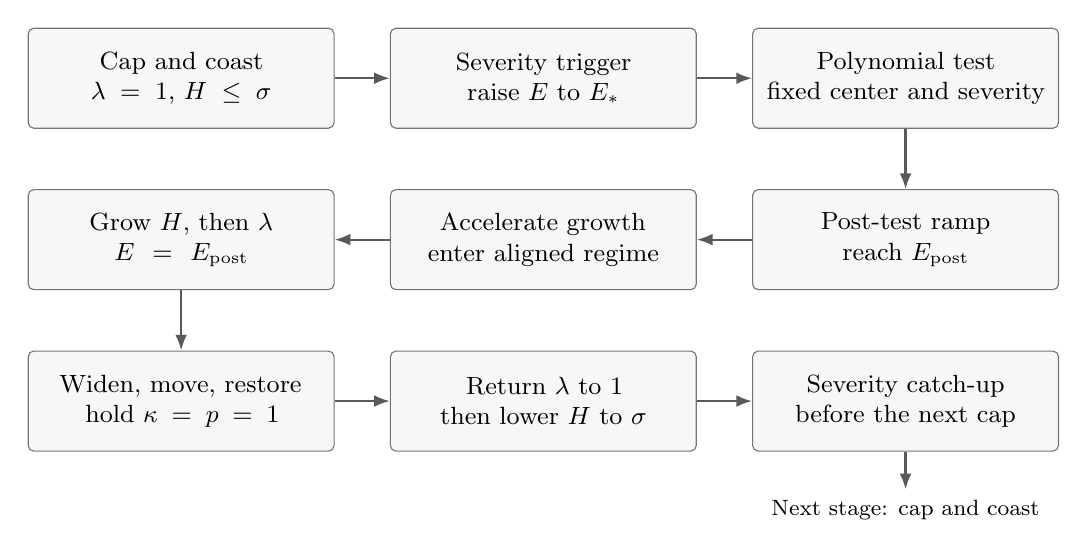
\begin{tikzpicture}[
  stage/.style={draw=black!55,rounded corners=2pt,fill=black!3,
    text width=3.65cm,minimum height=1.27cm,align=center,font=\small},
  flow/.style={-{Latex[length=2mm]},thick,draw=black!65},
  note/.style={font=\footnotesize,align=center}]
\node[stage] (cap) at (0,0) {Cap and coast\\
  $\lambda=1$, $H\le\sigma$};
\node[stage] (trigger) at (4.6,0) {Severity trigger\\
  raise $E$ to $E_*$};
\node[stage] (test) at (9.2,0) {Polynomial test\\
  fixed center and severity};
\node[stage] (post) at (9.2,-2.05) {Post-test ramp\\
  reach $E_{\rm post}$};
\node[stage] (accelerate) at (4.6,-2.05) {Accelerate growth\\
  enter aligned regime};
\node[stage] (grow) at (0,-2.05) {Grow $H$, then $\lambda$\\
  $E=E_{\rm post}$};
\node[stage] (center) at (0,-4.1) {Widen, move, restore\\
  hold $\kappa=p=1$};
\node[stage] (reset) at (4.6,-4.1) {Return $\lambda$ to $1$\\
  then lower $H$ to $\sigma$};
\node[stage] (catchup) at (9.2,-4.1) {Severity catch-up\\
  before the next cap};
\draw[flow] (cap)--(trigger);
\draw[flow] (trigger)--(test);
\draw[flow] (test)--(post);
\draw[flow] (post)--(accelerate);
\draw[flow] (accelerate)--(grow);
\draw[flow] (grow)--(center);
\draw[flow] (center)--(reset);
\draw[flow] (reset)--(catchup);
\draw[flow] (catchup.south)--++(0,-.48)
  node[below,note]{Next stage: cap and coast};
\end{tikzpicture}
\caption{One stage, in increasing spatial radius. The test is installed
while the spatial growth is capped. The intervening growth and center
change occupy finite clock intervals. After the reset, severity must
catch up with the accumulated spatial scale before the next capped
regime can begin. The arrows indicate order, not elapsed radius.}
\label{fig:stage-clock}
\end{figure}


We retain the radial notation of Lemma~\ref{radial:odes}:
\[
 \begin{gathered}
 t=|s|^2,\quad \nu=\log t,\quad a=B'(t),\quad u_s=\log a,\\
 Y=\frac{du_s}{d\nu},\quad a_\psi=\Psi'(t)=a/\lambda,\quad
 H=\frac{Y}{ta_\psi},\quad p=\frac{d\log a_\psi}{du_s}.
 \end{gathered}
\]
Here $H$ is a scalar; the polynomial system below is denoted by
$\mathcal H$. The evolution equations are
\begin{align}
 \frac{dY}{du_s}&=\kappa(1+Y),&
 \frac{d\nu}{du_s}&=Y^{-1},&
 \frac{d\log\lambda}{du_s}&=1-p,\label{assembly:clocks}\\
 \frac{d\Psi}{du_s}&=H^{-1},&
 \frac{d\log H}{du_s}
 &=\kappa(1+Y^{-1})-p-Y^{-1}.
 \label{assembly:H-clock}
\end{align}
The admissibility and derivative conditions on $\kappa,p$ in the radial
lemmas will always be imposed.

\subsection{Wells and the order of constants}

Fix a sequence $(\zeta_j,h_j)$ in which every pair from a fixed countable
dense subset of $\{|y|<1\}$ and $\mathbb Z_{\geq0}$ occurs infinitely
often. The parameters of a test will be
\begin{equation}\label{assembly:test-parameters}
 E_*=B_*c,\qquad \eta=e^{-c},\qquad
 N=\lfloor e^{\gamma E_*}\rfloor,\qquad
 l=\frac N2\log(t/R^2),\qquad S=Re^{c/N}.
\end{equation}
The constants $B_*,\gamma$ are fixed below. At each stage $R$ is fixed
before $c$. For a degree-$N$ system $(\mathcal H,p_N)$ from
Lemma~\ref{grid:polynomials}, define
\begin{equation}\label{assembly:well}
 W_j(s)=d\log
 \frac{|\mathcal H(s/R)|^2+|p_N(s/R)-1|^2+e^{-2c}}
 {1+e^{-2c}}.
\end{equation}
The polynomial $p_N$ is unrelated to the radial control $p$.
The logarithmic sum-of-squares formula shows that $W_j$ is smooth
and plurisubharmonic.

\begin{lemma}\label{assembly:well-bounds}
There is an absolute exponent $C_{\rm pol}$ such that, for $t\geq1$
and $1\leq r\leq4$,
\begin{equation}\label{assembly:well-raw}
 |\partial^{[r]}W_j|
 \leq C(n,d)\exp\{C_{\rm pol}(\max(l,0)+c+\log N)\}.
\end{equation}
There is a constant $L_n<\infty$ such that, after increasing the degree
threshold,
\begin{equation}\label{assembly:well-tail}
 |\partial^{[r]}W_j|\leq N^{L_n}
 \qquad(1\leq r\leq4,\ l\geq L_n\log N).
\end{equation}
Both statements hold throughout the indicated outer ranges.
\end{lemma}

\begin{proof}
Homogeneity and the spherical upper bound give
$|(\mathcal H,p_N)(s/R)|\leq Ne^l$. Cauchy estimates at scale
$c_0\sqrt t/N$ bound its derivatives of order at most four by this
quantity times a fixed power of $N$, since $t\geq1$. In a differentiated
logarithm there are only a fixed number of factors and denominator
powers; the denominator in \eqref{assembly:well} is at least $e^{-2c}$.
This proves \eqref{assembly:well-raw} with an absolute exponent;
fixed-dimensional constants and $d$ affect only its prefactor.

The spherical lower bound also gives
$|(\mathcal H,p_N)(s/R)|\geq e^lN^{-C_n}$. Once $l$ exceeds a sufficiently
large multiple of $\log N$, subtraction of $(0,1)$ leaves norm at least
$e^lN^{-C_n}/2$. The factors $e^l$ in derivatives of the logarithm can
then be canceled. The remaining costs are fixed powers of $N$, with
exponents depending on the already fixed $n$. Increase $L_n$ to pay
them and the degree threshold to pay the prefactor.
\end{proof}

For each stage we also introduce smooth nonnegative radial
plurisubharmonic functions $Z_{j,\rm in}$ and $Z_{j,\rm out}$. They
vanish before their stage and eventually become affine nondecreasing
functions of $\nu$. The center changes add offsets that vanish before
their change interval and are constant afterwards. We seek the final
twist in the form
\begin{equation}\label{assembly:twist}
 \psi=\Psi+\sum_j W_j+\sum_j(Z_{j,\rm in}+Z_{j,\rm out})
       +\text{center-change offsets}.
\end{equation}
The center is constant except on its change intervals. There is one
fiber profile at each spatial point: it is $q_0(x,E(s))$ except during
the coordinated switches of Proposition~\ref{center:change}.
Shears occur only in the disjoint test collars. The recursion below
will make the well sum converge smoothly on compact spatial sets;
the other added terms are locally finite.

The constants must provide the three outputs of
Proposition~\ref{grid:criterion}: a fixed-height spatial ball, small
unsheared disks on its boundary, and large prescribed sheared disks at
the nodes. Their exponents determine $k$ and hence the dimension.
Accordingly we first choose all geometric constants independently of
$n$, and only then use stagewise size choices to pay dimensional
prefactors.

We give the full order of choices. First choose the profile constants,
including $d_0,K_0$ for the center change, then $\epsilon,\mu$ for
Proposition~\ref{quiet:profile}, the shear exponent in
Proposition~\ref{quiet:shear}, and the tolerance $\delta$ for
Proposition~\ref{radial:aligned}. These choices are independent of $n$.
Use control transitions whose first two derivatives in $\log Y$ have
absolute bounds. Let $C_{\rm rad}$ dominate the absolute exponents
needed for radial raw jets through order four. Choose
\begin{equation}\label{assembly:first-constants}
 \epsilon_1\ll\epsilon/(1+C_{\rm rad}),\qquad
 C_\uparrow\gg(1+C_{\rm rad})/\epsilon.
\end{equation}
Choose next
\begin{equation}\label{assembly:second-constants}
 m_z\geq10(C_{\rm pol}+1),\qquad
 B_*\geq\frac{C_*(1+m_z+C_{\rm pol}+C_{\rm rad})}{\epsilon_1},
\end{equation}
where the absolute $C_*$ is large enough for the finitely many raw
exponent comparisons below. Choose $C_s$ larger than the quiet shear
severity exponent, and $C_w$ large enough to pay the shell loss and
four derivatives of its cutoffs; $C_w>5k_*+20$ suffices for these latter
costs after increasing the other fixed constants if necessary. Here
$k_*$ is the absolute separation exponent of the polynomial grids.
Choose
\begin{equation}\label{assembly:gamma-kb}
 0<\gamma\ll\epsilon_1,\qquad
 \gamma B_*\leq\min\{.005,(8C_w)^{-1}\},\qquad
 k_b>\max\{8/\gamma,100/\epsilon\}.
\end{equation}
Choose $M_b$ sufficiently large for the ratios in
Lemma~\ref{assembly:quiet-check}, and then $\sigma>0$ sufficiently small
for that lemma and Lemma~\ref{assembly:reset}. These are choices made
from fixed constants; in particular
$\sigma M_bk_b^2\ll1$, and $\sigma$ pays all quiet smallness requirements
involving $C_\uparrow$. Severity thresholds can depend on $\sigma$.
Finally take
\begin{equation}\label{assembly:depth}
 d\geq8(M_bk_b+C_s+1)B_*.
\end{equation}
All constants so far are independent of dimension.

Set
\begin{equation}\label{assembly:test-exponents}
 m_0=d/2,\qquad p_0=2d,\qquad
 p_1=C_sB_*+C_wd\gamma B_*.
\end{equation}
Then $p_1\leq d/4<m_0$. Choose an integer $k$ with
$.99k>p_0+p_1+1$, and only now fix a finite $n$ sufficiently large that
\begin{equation}\label{assembly:dimension}
 \sum_{r=1}^{k-1}\frac{r^{n-1}}{(n-1)!}<.01.
\end{equation}
Such a finite $n$ exists because $k$ is fixed. The constants $C_n,L_n$
and all dimensional prefactors will be paid by the stagewise choice
of large $c$; they do not change \eqref{assembly:test-exponents}.

\subsection{Recursive convention and capped intervals}

Every estimate for an already configured region is made with an
additional allowance of one for the absolute value and spatial
jets through order four of all future wells. Let $\nu_j^{\rm sat}$
denote the designated endpoint of severity saturation at stage $j$,
and let
\[
 K_j=\{s:|s|^2\leq e^{\nu_j^{\rm sat}}\}
\]
be the entire inner spatial ball ending there. The testing annulus lies
beyond this ball. At stage $j$ we impose
\begin{equation}\label{assembly:diagonal}
 \sup_{s\in K_j}|\partial^{[r]}W_j(s)|\leq2^{-j},
 \qquad 0\leq r\leq j+4.
\end{equation}
Each new trigger begins beyond every completed stage, so every already
configured region lies in every later $K_j$. The omitted well sum
therefore has absolute value and spatial jets through order four
bounded by $\sum_j2^{-j}\leq1$ there. Its Hessian is also positive
semidefinite. Feasibility is proved below. This convention reserves the
entire future allowance before selecting any future coefficients. We apply
the local all-fiber lemmas to the final twist with these allowances;
we do not infer a uniform curvature statement from small perturbations
on compact subsets of the total space.

Initially put
\begin{equation}\label{assembly:initial-data}
 a=a_\psi=a_{\rm init}e^t,\quad Y=t,\quad
 \lambda=p=1,\quad\kappa=(1+Y)^{-1},
\end{equation}
with $a_{\rm init}$ so large that $H\leq\sigma$, and choose $B,\Psi$
with equal initial constants. Up to a positive scale and an additive
constant, this initial spatial potential is the exponential radial
example of \citet[Section~3]{Seshadri2006}. Take center $\zeta_1$ and a constant
severity sufficiently large for the initial compact region and the
tail allowance. The radial curvature formula is strictly positive
on nonzero rank-two Hermitian tests at $t=0$, by its limit or by
direct differentiation of $a_{\rm init}e^t$. Thus the quiet criterion
also applies at the spatial origin.

Before every trigger the radial data will have the form
\begin{equation}\label{assembly:cap}
 \lambda=p=1,\qquad
 \kappa=\frac{C_\kappa}{1+Y},\qquad
 1\leq C_\kappa\leq1+Y,\qquad H\leq\sigma,
\end{equation}
with $C_\kappa$ constant on that interval. Then
$dY/d\nu=C_\kappa Y$, so the cap can be continued through any
prescribed finite interval of $\nu$ without a pole. All previously
generated nonradial twist terms have bounded positive-order Euclidean
jets on the entire outer range: use \eqref{assembly:well-tail} and
the affine $Z$ tails. Hence a cap can also be continued until
$a=e^{u_s}$ dominates any prescribed bound for those old jets.

Choose the next trigger start $\nu_B$ with
$Y_B=Y(\nu_B)\gg C_\kappa$, $e^{\nu_B}\geq1$, and severity constant
there at a value satisfying
\begin{equation}\label{assembly:trigger-initial}
 E_0\geq C_\uparrow u_s(\nu_B).
\end{equation}
The reset below provides this inequality and any additional fixed
threshold. Put
\begin{equation}\label{assembly:trigger-radius}
 \xi=Y_B(\nu-\nu_B),\qquad
 \nu_*=\nu_B+Y_B^{-1},\qquad R=e^{\nu_*/2}.
\end{equation}
These data precede the choice of $c$. Retain the capped radial data
through
\begin{equation}\label{assembly:post-length}
 l=T_*+4,\qquad T_*=10\{c+(1+L_n)\log N\}.
\end{equation}
For large $c$ this lies inside $\nu\leq\nu_B+2/Y_B$, since
$(T_*+4)/N\to0$. Throughout this fixed continuation
$Y\asymp Y_B$ and $u_s=u_s(\nu_B)+O(1)$, with constants allowed
to depend on the already fixed cap data.

\begin{lemma}\label{assembly:height}
Before choosing $c$ at stage $j$, one can fix $D_j\geq j$ such that,
for every sufficiently large permitted $c$ and every final choice of
the reserved tails,
\begin{equation}\label{assembly:height-bound}
 \ell(s,\zeta_j)\leq D_j-2\qquad(|s|\leq Re^{c/N}).
\end{equation}
\end{lemma}

\begin{proof}
On the spatial region following the previous center-change interval,
the center is $\zeta_j$ and $\ell(s,\zeta_j)=B(s)$, including on shear
supports. The same identity holds on the initial cap at the first
stage. Thus the bound there follows from the fixed cap continuation
up to $\nu_B+2/Y_B$.
The earlier spatial region is a fixed compact set $K$ with already
chosen profiles and centers; future stages do not change $q(x,s)$
on $K$. The reservation gives $|\psi-\psi_{\rm old}|\leq1$ there,
including the current and all later wells. Both centers are in the unit disk, so
$|\zeta_j-\zeta(s)|\leq2$. Choose
$A>\log4+\sup_K\psi_{\rm old}+1$.
For each $s\in K$, $F(x,s)\to\infty$ as $x\to\infty$.
Continuity, a finite cover, and monotonicity in $x$ give a common
finite $X$ with $F(X,s)>A$ on $K$. Inverting the fiber relation
therefore gives $\tau\leq e^X$. Since $q\geq1$, the radial potential
is bounded by $\sup_K B+e^X$; the fixed shear adds at most
$2\sup_K|c_{\rm sh}|$. At center coincidences this argument is
understood by the smooth limit $\tau=0$. These bounds are independent
of $c$ and of the future wells. Add two and increase to at least $j$.
\end{proof}

We always require
\begin{equation}\label{assembly:height-rate}
 c\geq j(D_j+1)
\end{equation}
in addition to the finitely many current thresholds. Thus $D_j\to\infty$
and $D_j/c_j\to0$.

\subsection{The severity trigger}

Choose a smooth convex nondecreasing $h_b$ on $(-\infty,1)$, zero
for $\xi\leq0$, equal to $-\log(1-\xi)$ up to an affine function near
$1$. To construct it, cut on the nonnegative second derivative
$(1-\xi)^{-2}$ smoothly and integrate twice from zero.
Use
\begin{equation}\label{assembly:trigger}
 E=E_0+k_bh_b(\xi),\qquad Z_{j,\rm in}=M_bk_b^2h_b(\xi)
\end{equation}
until severity is near $E_*$. Smoothly saturate $E$ at $E_*$ over
a unit interval of its argument, so that $E=E_*$ by
$k_bh_b=E_*-E_0+1$. Derivatives of the saturation function in that
argument are bounded. Keep the unsaturated convex $Z_{j,\rm in}$
slightly longer, and once $k_bh_b\geq E_*-E_0+2$, cut off its
second derivative nonnegatively over half the remaining gap to
$\xi=1$. Continue it affinely in $\nu$ thereafter. This is a smooth
convex nondecreasing function. Such a function of $\log|s|^2$,
zero near the origin, is a smooth radial plurisubharmonic function:
its transverse and radial Hessian entries are its first and second
$\nu$ derivatives divided by $t$.

Near this cutoff the gap $1-\xi$ is comparable, with fixed stagewise
factors, to $e^{-(E_*-E_0)/k_b}$. The final slope is bounded by
\begin{equation}\label{assembly:trigger-slope}
 C M_bk_b^2Y_Be^{(E_*-E_0)/k_b}.
\end{equation}
The value there is $M_bk_b(E_*-E_0+O(1+k_b))$. Multiplication
of \eqref{assembly:trigger-slope} by the remaining gap to $\nu_*$
costs only a fixed $O(M_bk_b^2)$, and its product with $4c/N$
tends to zero. Thus for large $c$,
\begin{equation}\label{assembly:trigger-value}
 Z_{j,\rm in}\leq2M_bk_bE_*\qquad(|l|\leq2c).
\end{equation}
Through saturation, its derivatives and those of $E$ through order
four have bounds given by fixed prefactors times
$(1+Y_B)^4 e^{4(E-E_0)/k_b}$.
The bound with $E_*$ also holds for positive-order derivatives of
the affine tail.

The well satisfies \eqref{assembly:diagonal} after increasing $c$.
Indeed throughout severity saturation,
\begin{equation}\label{assembly:activation-gap}
 l\leq-C(Y_B,E_0)N e^{-E_*/k_b}.
\end{equation}
The absolute value on the right grows exponentially in $E_*$,
because $\log N\sim\gamma E_*$ and $\gamma>4/k_b$.
Homogeneity makes the polynomial evaluations on the whole inner
ball exponentially small in this quantity. Cauchy on a collar
of scale $R/N$ gives the same conclusion for any fixed derivative
order, with only powers of $N$ as further costs. The logarithm in
\eqref{assembly:well} is then close to zero with all these
derivatives. We can therefore enforce the bound $2^{-j}$ for its
value and derivatives through order $j+4$. This decay pays all
fixed exponential-in-$c$ costs needed at stage $j$.

\begin{lemma}\label{assembly:quiet-check}
The trigger satisfies the hypotheses of
Proposition~\ref{quiet:profile}, uniformly for every $\tau\geq0$.
After saturation the same criterion applies through $l=4c$, including
the initial part of the post-test term defined below.
\end{lemma}

\begin{proof}
For raw estimates use Euclidean axes. Here $t\geq1$, $Y\asymp Y_B$,
and $\log Y_B\leq C u_s(\nu_B)$; the last estimate follows by
integrating $d\log Y/du_s=\kappa(1+Y^{-1})\leq2.2$ for $Y\geq1$.
Differentiation of $a'=aY/t$ bounds the required radial metric jets
by $e^{C_{\rm rad}u_s}$. Their inverses cost no more. The radial
curvature estimate gives
\begin{equation}\label{assembly:euclidean-curvature}
 C^V(T,T)\geq c\kappa H|T|_V^2
 \geq c(a/t)|T|^2,
\end{equation}
since $V\geq aI$ and
$\kappa H=C_\kappa Y/((1+Y)ta)\geq c/(ta)$.
The initial severity pays these bounds, the old data and the future
allowance. The trigger cost $e^{4E/k_b}$ fits the quiet raw exponent.
The current well is small before saturation. Also $G\geq V$, since
all nonconstant extra twist terms in this interval are
plurisubharmonic.

For the covariant condition, write
\[
 \mathcal B(\nu)=B(e^\nu),\qquad
 \mathcal U(\nu)=\Psi(e^\nu)+Z_{j,\rm in}(e^\nu),
\]
and use primes for $\nu$ derivatives within this proof. On the
severity-varying interval,
\begin{align}
 \frac{\mathcal U''}{\mathcal U'},\
 \frac{|\mathcal U'''|}{\mathcal U''},\
 \frac{\mathcal B''}{\mathcal B'},\
 \frac{|\mathcal B'''|}{\mathcal B''}
 &\leq C\sqrt{\mathcal U''},
 \label{assembly:connection-ratios}\\
 \frac{|E'|}{\mathcal U'},\
 \frac{|E'|}{\sqrt{\mathcal U''}},\
 \frac{|E''|}{\mathcal U''},\
 \frac{|E'''|}{(\mathcal U'')^{3/2}}
 &\leq\varepsilon_b,
 \label{assembly:small-ratios}
\end{align}
where $\varepsilon_b$ can be made as small as required.
Away from the pole, $h_b$ and its relevant derivatives are bounded,
whereas
$\mathcal B'=Y/H$ and $\mathcal B''=Y(1+Y)/H$.
The choice $\sigma M_bk_b^2\ll1$ makes these background terms
dominate. Near the pole let $D_b=Y_B/(1-\xi)$. Then
\[
 Z_{j,\rm in}'\asymp M_bk_b^2D_b,\quad
 Z_{j,\rm in}''\asymp M_bk_b^2D_b^2,\quad
 |Z_{j,\rm in}'''|\leq C M_bk_b^2D_b^3,
\]
and $|E^{(r)}|\leq Ck_b^rD_b^r$ for $1\leq r\leq3$, including
saturation. These prove \eqref{assembly:connection-ratios} and
make \eqref{assembly:small-ratios} small by first enlarging $M_b$
and then decreasing $\sigma$. The fixed intervening interval of
$\xi$ is covered by the first estimates. We also have
$\mathcal U''\geq1$.

At fixed $\tau$, the radial part of the Schur metric is the Hessian of
\[
 J_h=\mathcal B+\tau(\mathcal U-\bar F(x,E)),
\]
where the bar denotes averaging from zero to $\tau$ in the $\tau$
variable. Bounded severity derivatives of $\bar F$ and
\eqref{assembly:small-ratios} show that the first two derivatives
of $\mathcal U-\bar F$ are positively comparable with those of
$\mathcal U$ and its third derivative is bounded by
$C(\mathcal U'')^{3/2}$.
Use affine axes normalized by the Hessian of $\mathcal U$, with
radial radius $\sqrt{t/\mathcal U''}$ and transverse radii
$\sqrt{t/\mathcal U'}$.
At a radial point, the only nonzero holomorphic connection types
for a radial Hessian metric are radial--radial to radial and
radial--transverse to transverse. Differentiation gives the bounds
\begin{equation}\label{assembly:connection-exact}
 \frac{|J_h'''/J_h''-1|}{\sqrt{\mathcal U''}},
 \qquad
 \frac{|J_h''/J_h'-1|}{\sqrt{\mathcal U''}}.
\end{equation}
They are bounded by \eqref{assembly:connection-ratios}. No estimate
of a radial/transverse condition number is used.

Write the remaining Hessian as $\tau G_e$, with $G_e\geq0$.
Its size and first jets in these axes are bounded: old Euclidean
bounds are dominated by the large initial $a$, and the current
and future wells have the reserved absolute bounds. The normalizing
radii are at most $a^{-1/2}$ because this background is at least
$V\geq aI$. If $h_r$ denotes the radial Schur metric, the exact
connection difference is, with the usual index placement,
\begin{equation}\label{assembly:connection-perturbation}
 \Gamma^h-\Gamma^{h_r}
 =\tau(\partial G_e-\Gamma^{h_r}G_e)(h_r+\tau G_e)^{-1}.
\end{equation}
Since $h_r\geq c\tau I$, $\tau h^{-1}$ is uniformly bounded for
all $\tau>0$. Thus the full connection is uniformly bounded as well.

In these axes the first derivative of $E$ has norm
$|E'|/\sqrt{\mathcal U''}$; the complex Hessian entries are bounded
by $|E'|/\mathcal U'$ and $|E''|/\mathcal U''$, and the only pure
second derivative has size $|E''-E'|/\mathcal U''$.
Consequently subtracting the connection times the first derivative
gives a small $\nabla_h^{2,0}E$. Since the actual $G$ is at least the
normalizing background, the same smallness holds in $G$ units.
This proves all quiet smallness conditions uniformly in $\tau$.

After saturation, severity derivatives vanish. Through $l=4c$ the
well's raw costs are bounded by $e^{C(c+\log N)}$; the post term
below has cost at most a fixed multiple of $N^4e^{2m_zc}$.
Both fit $\epsilon E_*$ by \eqref{assembly:second-constants}, while
the inverse and radial curvature estimates persist.
\end{proof}

\subsection{Testing disks and the post ramp}

Choose $c$ sufficiently large that the degree in
\eqref{assembly:test-parameters} meets the grid accuracy required for
$h_j$, and $N>h_j$. At every good lift $v$, use a smooth cutoff
supported in $|s-Rv|<2RN^{-k_*}$ and equal to one on
$|s-Rv|\leq RN^{-k_*}$. Assign on the inner ball
\begin{equation}\label{assembly:shear-amplitude}
 c_{\rm sh}=\alpha b_v,\qquad
 \alpha=\exp(-C_sE_*-C_wd\log N),
\end{equation}
and multiply by the cutoff in the collar. The phases have modulus
one, are independently assignable by projective direction, and
repeat on every lift of that direction. The outer balls are disjoint.
A cutoff $\chi(|s-Rv|^2/(RN^{-k_*})^2)$ has fixed-order multilinear
derivative bound $C_r(RN^{-k_*})^{-r}$ with absolute $C_r$.
At most one contributes at any point, so there is no factor for
the number of nodes or dimension.

On the derivative supports, the shell estimate gives
\begin{equation}\label{assembly:shear-lower}
 \psi\geq-2d(k_*+11)\log N-C_{\rm old}.
\end{equation}
Old values are bounded on the fixed cap continuation, future values
have the allowance, and the trigger term is nonnegative.
These balls have $|l|\leq\log N+1$ and lie beyond severity
saturation. First and pure second derivatives of $\psi$ also fit
the quiet raw bounds; the extra background first-derivative cost
is at most $a\sqrt t$. The constants $C_s,C_w$ pay respectively
the severity exponent of Proposition~\ref{quiet:shear} and half the
loss \eqref{assembly:shear-lower} together with the four cutoff
derivatives. Large $c$ pays fixed old factors. Thus that proposition
applies for all fiber radii with metric comparison loss at most
$1/2$. Where a shear coefficient is constant, its potential term
is pluriharmonic.

At a node the new well is $-2dc+O(1)$; on $|s|=S$ it is at most
$2d(c+\log N)+O_d(1)$. All other values on the fixed continuation
are bounded independently of $c$, except the trigger term.
The post term is still zero. Hence
\begin{align}
 \psi_{\rm node}&\leq-2dc+2M_bk_bB_*c+C_{\rm old},
 \label{assembly:node-twist}\\
 \psi_{\rm sphere}&\leq2d(c+\log N)+2M_bk_bB_*c+C_{\rm old,d}.
 \label{assembly:sphere-twist}
\end{align}
For a small fixed profile-dependent $c_0>0$, the disk
\begin{equation}\label{assembly:fiber-disk}
 |y-\zeta_j|<c_0e^{-(\psi+E_*)/2}
\end{equation}
has $\tau\leq e^{-E_*}$ and radial potential increment at most one.
Indeed, by the axis estimates in Lemma~\ref{quiet:scalar}, at
$\tau=e^{-E_*}$ the normalized relation gives $F=-E_*+O(1)$ uniformly: integrate $1/q-1=O(e^{E_*}\tau)$
up to that value of $\tau$. Monotonicity proves the disk assertion.

At a node the holomorphic shear
$w\mapsto w+i\alpha b_v(y-\zeta_j)$ has imaginary increment
$\operatorname{Re}(\alpha b_v(y-\zeta_j))$, exactly the added
potential. Writing $z=y-\zeta_j$, the clearance on the disk
\eqref{assembly:fiber-disk}, over any $w$ with
$\operatorname{Im}w=D_j$, is therefore
\[
 \begin{split}
 &\operatorname{Im}(w+i\alpha b_vz)
       -\ell(Rv,\zeta_j+z)\\
 &\qquad=D_j-\ell_{\rm rad}(Rv,\zeta_j+z)
       \geq D_j-B(Rv)-1\geq1.
 \end{split}
\]
The last inequality uses \eqref{assembly:height-bound} on the center
axis. Thus the shear consumes none of the height margin, and the
sheared disk lies in the tube. Its logarithmic radius is at least
\[
 (d-M_bk_bB_*-B_*/2)c-C_{\rm old}
 \geq(13d/16)c-C_{\rm old},
\]
which exceeds $m_0c$ for large $c$.
On the sphere there is no shear, and Cauchy's inequality on
\eqref{assembly:fiber-disk} bounds the transverse derivative
of a function of modulus at most one by
\[
 \exp\{[d(1+\gamma B_*)+M_bk_bB_*+B_*/2]c+C_{\rm old,d}\}
 \leq e^{p_0c}.
\]
Also $\alpha^{-1}\leq e^{p_1c}$.
These are precisely the constants \eqref{assembly:test-exponents},
with strict margins to absorb the prefactors.
Choose the phases supplied by Proposition~\ref{grid:criterion}.
All geometric estimates hold for arbitrary phases.

For the post ramp, add a smooth convex nondecreasing function
$Z_{j,\rm out}$ of $l$, zero through $2c$, and equal to
$e^{m_z(l-2c)}$ up to affine terms from $2c+2$ onward.
This is obtained by cutting on its positive second derivative and
integrating twice. Continue through $T_*+2$, then cut off that
second derivative nonnegatively so that the function is affine
after $T_*+3$. Independently turn on the severity slope $B_*$
in $l$ over $[4c,4c+1]$, and turn it off over
$[T_*,T_*+1]$. Write $E_{\rm post}$ for the final value.
For large $c$,
\begin{equation}\label{assembly:post-severity}
 E\geq B_*(c+l)/10\quad(2c\leq l\leq T_*+4),\qquad
 E_{\rm post}\geq B_*T_*/2.
\end{equation}

\begin{lemma}\label{assembly:post}
The quiet criterion holds throughout the post ramp.
Beyond $l=T_*+4$, the sum of all already generated additive twist
terms other than $\Psi$ and the constant offsets, and each such
term individually, has Euclidean positive-order jets through order
four bounded on the whole outer range by
\begin{equation}\label{assembly:outer-bound}
 D_{\rm out}=\exp(\epsilon_1E_{\rm post}/3).
\end{equation}
\end{lemma}

\begin{proof}
Each derivative of a function of $l$ costs a fixed power of $N$.
Thus $Z_{j,\rm out}$ has positive-order bounds through order four
of size $C N^4e^{m_z\max(0,l-2c)}$. These and
\eqref{assembly:well-raw} fit the raw quiet exponent by
\eqref{assembly:second-constants} and \eqref{assembly:post-severity}.
Other radial and old-data bounds remain fixed on the cap
continuation. Through $l=4c$, severity is constant and the preceding
lemma applies.

Where severity varies, take $\mathcal U=\Psi+Z_{j,\rm out}$.
Before division by $t$, its transverse and radial Hessian entries
have sizes
\[
 m_zN e^{m_z(l-2c)},\qquad
 (m_zN)^2e^{m_z(l-2c)}.
\]
For $l\geq4c$, $m_z(l-2c)$ exceeds
$C_{\rm pol}(l+c+\log N)$ by a fixed positive multiple of $c+l$.
Thus this Hessian dominates the current well and its first
Hessian jets in normalized axes.
The affine $Z_{j,\rm in}$ tail has coefficient at most a fixed
factor times $e^{E_*/k_b}\ll N$; old terms and future tails are
covered as before. Moreover
$\mathcal U''/\mathcal U',|\mathcal U'''|/\mathcal U''\leq Cm_zN$,
while $\sqrt{\mathcal U''}\gtrsim
m_zN e^{m_z(l-2c)/2}$.
Severity derivatives of orders $r\leq3$ are at most $CB_*N^r$.
Thus the connection ratios hold and all severity ratios are small.
Equations~\eqref{assembly:connection-exact} and
\eqref{assembly:connection-perturbation} again prove the pure
Hessian condition uniformly for all $\tau$. Every extra Hessian
is positive semidefinite in this interval.

Past $T_*+4$ the new well satisfies \eqref{assembly:well-tail},
and the $Z$ terms are affine in $\nu$. Their positive-order
Euclidean jets are bounded on the entire outer range by their
endpoint bounds up to fixed constants. Their logarithmic costs
are at most
$C(1+m_z)T_*+4\log N+C_{\rm old}$ with an absolute $C$.
The absolute constant $C_*$ in \eqref{assembly:second-constants}
was chosen to pay this inequality too.
Equation~\eqref{assembly:post-severity} then implies
\eqref{assembly:outer-bound}, after increasing $c$ for the finite
sum of old bounds, the number of generated terms, and dimensional
prefactors. The dimension-dependent $L_n$
multiplies $T_*$ on both sides and changes no leading comparison.
\end{proof}

\subsection{Acceleration, center change, and reset}

At constant $E_{\rm post}$, increase $\kappa$ from the cap value
to $\kappa_*=1.08$ on a fixed-factor interval of $Y$ after
$l=T_*+4$, keeping $\lambda=p=1$. The transition can preserve
$Y\kappa_Y\geq-\kappa$: multiply the difference between the cap
value and $\kappa_*$ by a nondecreasing cutoff in $\log Y$.
The upward derivative only improves that inequality.
The $u_s$ increment is bounded in terms of the fixed prior $Y_B$,
independently of large $c$. Keep $\kappa=\kappa_*$ until
\begin{equation}\label{assembly:aligned-entry}
 u_s=\epsilon_1E_{\rm post}.
\end{equation}
For large $c$ this endpoint lies after the transition and has
$H\geq\sigma$. Indeed, with $p=1$,
$d\log H/du_s=(\kappa_*-1)(1+Y^{-1})\geq.08$,
whereas the initial values at the end of the cap have fixed
stagewise bounds as $c\to\infty$.

Until \eqref{assembly:aligned-entry}, apply the quiet criterion.
The radial raw jets cost $e^{C_{\rm rad}u_s}$, the extra twist
jets are bounded by \eqref{assembly:outer-bound}, and the curvature
lower bound follows as in \eqref{assembly:euclidean-curvature}.
Severity derivatives vanish. The choices of $\epsilon_1$ and $B_*$
pay all these estimates. At entry $a_\psi=e^{\epsilon_1E_{\rm post}}$.
By the scaled-axis estimate of the radial lemmas, an extra
Euclidean Hessian with two further jets bounded by $D$ costs at
most $CD/(a_\psi H)$ in scaled axes. Consequently at entry and
through the later aligned intervals,
\begin{equation}\label{assembly:aligned-extra}
 |j^{\leq2}G_e|_{\rm scaled}\leq\delta/H.
\end{equation}
Here we leave a fixed fraction of the $\delta$ budget for future
wells. The ratio $D_{\rm out}/a_\psi$ is exponentially small at
entry and only decreases later, since $a_\psi$ increases.
During an actual profile switch its new offset is accounted for
by Proposition~\ref{center:change}; outside the switch, that offset
is constant.

\begin{lemma}\label{assembly:change-order}
At constant $E_{\rm post}$ the center can be changed from $\zeta_j$
to $\zeta_{j+1}$, and the data can then be restored to
\[
 \lambda=p=1,\qquad \kappa=1,\qquad H=\sigma,
\]
using finite clock intervals and only the aligned and center-change
regimes. The old-twist bounds needed for choosing the profile
shift are available independently of the targeted $\lambda,H$.
\end{lemma}

\begin{proof}
Initially grow $H$ with $\kappa=\kappa_*$ and $p=\lambda=1$.
Use the $\lambda=1$, $H\geq\sigma$ alternative of
Proposition~\ref{radial:aligned}. Ultimately we will lower $p$
slightly below one for a bump, thereby increasing $\lambda$, and
then restore $p=1$ and return smoothly to $\kappa=1$.

We first justify the order in which the targets are chosen.
During the growth and the bump, $p\leq1$ and $\kappa=\kappa_*$,
so $d\log H/du_s\geq.08$. Thus
\[
 \int_{u_{\rm entry}}^\infty \frac{du_s}{H}
 \leq \frac{1}{.08H_{\rm entry}}.
\]
This bounds the total increase of $\Psi$ before the final transition
independently of the size of either target. The transition from
$\kappa_*$ to one takes a fixed $\log Y$ interval and leaves
$H$ nondecreasing, adding another fixed bound to $\Psi$.
Moreover $\kappa\geq1$ gives
$d\log Y/du_s\geq1$, hence
\[
 0\leq\nu-\nu_{\rm entry}
 =\int \frac{du_s}{Y}\leq Y_{\rm entry}^{-1}
\]
through the growth and holding intervals. The old nonradial
twists therefore have bounded values on one fixed compact
spatial interval, independently of the targets. Their scaled
derivatives are bounded by the fixed Euclidean bounds, since
the scaled coordinate radii are at most one. Derivatives of
$\Psi$ in these axes are $O(1/H)\leq O(1/\sigma)$.
The forward switch and center move each occupy a fixed amount
of the variable $\Psi$; these amounts can be included in the
same bounds. Include the reserved future value and jet allowance
as well. These are exactly old-twist bounds independent of
$\lambda,H$, as required by Proposition~\ref{center:change}.

Choose its shift $L_0$ from these bounds and $E_{\rm post}$.
This fixes its profile constants $C_f$ and a sufficient target
$\lambda$, and that target determines a sufficient target $H$.
This is the order of parameter selection in
Proposition~\ref{center:change}. The radial path reaches the targets
in the other order: grow $H$ first until it exceeds every required
multiple of
\[
 C_{E_{\rm post}}(1+\log\lambda)^2
 \quad\hbox{and}\quad C_f(1+\log\lambda)^2.
\]
Choose a smooth bump of $1-p\geq0$ with small amplitude and
small derivatives in $\log Y$, and with integral in $u_s$
equal to the desired $\log\lambda$. Such a bump exists by
making its middle plateau arbitrarily long; the endpoint ramps
can have fixed small amplitude and sufficiently long fixed
length, while the plateau length supplies the remaining integral.
The conversion $d\log Y/du_s=\kappa(1+Y^{-1})$ and its bounded
derivatives show that bounds through order two in $\log Y$
follow from the same bounds in $u_s$.
Throughout this bump $H$ increases, and the already chosen lower
bound for $H$ pays the entire range $0\leq\log\lambda(s)\leq
\log\lambda$. Apply the large-$H$ alternative of
Proposition~\ref{radial:aligned}.

Restore $p=1$ and lower $\kappa$ smoothly to one. The downward
transition can be made slowly enough in $\log Y$ that
$Y\kappa_Y\geq-\kappa$, with absolute derivative bounds.
Since $\kappa\geq1$ here, $H$ stays large. Now $\kappa=p=1$,
so both $H$ and $\lambda$ are constant. Perform the forward
profile switch, the center move, and the reverse switch of
Proposition~\ref{center:change}. Interpolate the two center
values by a flat-ended convex combination, keeping the center
in the unit disk. The old bounds and targets have been chosen
in the order just proved. The changes take a bounded interval
of $\Psi$, hence a finite interval of $u_s$ because
$d\Psi/du_s=1/H$ and $H$ is fixed, even though this interval
can be very long. Restore $q_0$ and retain the new constant
offset. The center is now $\zeta_{j+1}$. The offset may be arbitrarily
large, but it is now constant and changes no derivative of the twist. Its
value becomes part of the old data when the next testing height is
chosen, before the next accuracy parameter $c$.

Raise $\kappa$ to $\kappa_*$ again and use a bump with
$1<p<\kappa_*$ to bring $\log\lambda$ down to zero.
A small positive plateau and fixed ramps give any prescribed
finite integral of $p-1$; stop precisely when that integral
equals the existing $\log\lambda$. Thus $\lambda$ never falls
below one. Also
\[
 \frac{d\log H}{du_s}
 =\kappa_*-p+\frac{\kappa_*-1}{Y}>0,
\]
so the large-$H$ aligned condition remains valid. Restore $p=1$.

Finally reduce $H$ to $\sigma$. Transition $\kappa$ to $1/2$,
hold there for an adjustable interval, then return to one from
below. For $p=1$ the exact relation is
\begin{equation}\label{assembly:H-descent}
 \frac{d\log H}{d\log Y}=1-\kappa^{-1}.
\end{equation}
Its value is $-1$ on the middle plateau. The endpoint transitions
have fixed finite effects on $\log H$; the initial $H$ can be
made as large as needed. Choose the plateau length so that the
final value is exactly $\sigma$. Throughout this descent
$H\geq\sigma$, $\lambda=1$, and $1/2\leq\kappa\leq\kappa_*$,
so the $\lambda=1$ aligned alternative applies. Choose the
downward transitions slowly enough to preserve the same
derivative inequality as above.

All these intervals have finite $u_s$ or finite $\log Y$ length.
Equations~\eqref{assembly:clocks} show that $Y$ remains finite
on each finite $u_s$ interval and that the radius advances by
a finite positive amount. A putative pole of an indefinitely
continued accelerated equation is therefore never reached
during an episode. This proves the claim.
\end{proof}

\begin{lemma}\label{assembly:reset}
From the endpoint in Lemma~\ref{assembly:change-order}, severity
can be increased and a new cap started so that the next trigger
has \eqref{assembly:trigger-initial}, while the metric continues
to satisfy the quiet criterion. The cap can be extended to
arbitrarily large spatial radii.
\end{lemma}

\begin{proof}
The spatial scale $u_s$ may now be enormous, and $E_{\rm post}$ need
not dominate it. Proposition~\ref{quiet:profile} permits any fixed
holomorphic affine frame at the evaluation point. We first use
$V$-unit affine axes, where the curvature scale is the fixed $\sigma$
and the relevant jets are bounded independently of $u_s$. This will
justify the initial severity increase before arranging the size
inequality needed for the next trigger.

First hold $\kappa=p=\lambda=1$ and $H=\sigma$.
Let $E$ increase smoothly as a function of $u_s$, starting at
$E_{\rm post}$, with a fixed flat-ended transition to slope
$4C_\uparrow$. Its derivatives through order four in $u_s$
are bounded by constants depending on the fixed parameters,
not on $\sigma$ or the possibly enormous $u_s$ at entry.
Continue long enough that
\begin{equation}\label{assembly:catchup}
 E\geq2C_\uparrow u_s
\end{equation}
and any desired fixed threshold. The greater slope ensures
that this occurs after a finite interval.

We verify the quiet criterion even before \eqref{assembly:catchup}.
Use $V$-unit affine axes. The scaled-jet radial estimates give
metric jets of orders $r=1,2$ bounded by $CH^{r/2}$ in these
axes, and scaled derivatives of $u_s$ through order four are
bounded by an absolute constant. Therefore
\[
 |\partial^{[r]}E|_{V}\leq C H^{r/2},\qquad 1\leq r\leq4.
\]
The extras in \eqref{assembly:aligned-extra} satisfy the same
bounds after this normalization, and $G\geq V$.
For $\sigma$ small, the severity terms in $\mathcal N$ are
small relative to $G$, so
$h\asymp(1+\tau)V$, with first derivatives bounded in these
axes by $C(1+\tau)\sqrt H$.
Its connection is consequently $O(\sqrt H)$ uniformly in
$\tau$. The first, complex second, and pure covariant second
severity derivatives are small for every $\tau$.

The raw curvature margin on this hold is
$C^V(T,T)\geq c\sigma|T|^2$ in $V$-unit axes, because
$\kappa=1$ and $H=\sigma$. All other raw data are bounded there
by fixed constants. The previously chosen $E_{\rm post}$
exceeds the fixed profile and $\sigma$ thresholds, so it
pays this margin even when it is much smaller than the current
$u_s$. Thus there is no gap before severity catches up.

After \eqref{assembly:catchup}, keep the same slope while
turning $\kappa$ into a cap. Here is an explicit admissible
transition. If $Y_0$ is its starting clock value, set
\[
 A(Y)=1+Y_0+\int_{Y_0}^Y \eta_0(v/Y_0)\,dv,\qquad
 \kappa(Y)=\frac{A(Y)}{1+Y},
\]
where $\eta_0$ is smooth, equals one near $1$, decreases
nonnegatively to zero, and is zero for arguments at least two.
For $Y\leq Y_0$ use $A=1+Y$.
Then $1\leq A\leq1+Y$, so
$(1+Y)^{-1}\leq\kappa\leq1$. Moreover
\[
 Y\kappa_Y+\kappa
 =\frac{YA'(Y)}{1+Y}+\frac{A(Y)}{(1+Y)^2}\geq0.
\]
The first two derivatives of $\kappa$ in $\log Y$ have absolute
bounds, because $Y/Y_0$ ranges over a fixed interval while
$\eta_0$ changes. For example, writing $b=Y/(1+Y)$ and
$D=Y\partial_Y$, one has
$D\kappa=b(\eta_0-\kappa)$ and
$D^2\kappa=b(1-2b)(\eta_0-\kappa)+bD\eta_0$.
At the end $A$ is the new constant $C_\kappa$.
Since $\kappa\leq1$ and $p=1$, $H$ is nonincreasing and
stays at most $\sigma$.

The same normalized jet and connection estimates continue
through the transition and the cap. To check the raw curvature
margin there, note that $Y\geq t$: it holds initially, and
$d\log Y/d\nu=\kappa(1+Y)\geq1$ preserves it.
Also $u_s\geq t$ after choosing the initial constant large
enough, since $du_s/dt=Y/t\geq1$.
Hence
\[
 \kappa H\geq c/(ta)\geq c e^{-2u_s}
 \quad(t\geq1),
\]
and \eqref{assembly:catchup} with large $C_\uparrow$ pays the
quiet lower bound $e^{-\epsilon E}$. The positive-order
extras stay bounded relative to $V$ on an arbitrarily long
cap. More explicitly, a fixed Euclidean jet bound $D_{\rm out}$
costs at most
$C(D_{\rm out}/a)H^{r/2}$ in $V$-unit axes for Hessian jets
of order $r\leq2$, since $aH=Y/t\geq1$.
The ratio only decreases as $a$ grows.
Future wells are included in the fixed allowance until
their own activations.

Coast as far in $\nu$ as desired. Shortly before the next
chosen trigger, turn off the severity slope smoothly over
a fixed-length $u_s$ interval. The margin in
\eqref{assembly:catchup} is sufficient to retain
$E_0\geq C_\uparrow u_s(\nu_B)$ after this bounded final
increment, by making the cap endpoint large enough.
The existing raw jet bounds can also be absorbed by making
that endpoint large. This produces
\eqref{assembly:trigger-initial} and the next cap data.
\end{proof}

\subsection{Global realization and completeness}

We now carry out the recursion. At each stage first extend the
cap so that its trigger starts beyond all previous stages and
with $\nu_B\geq j$. Fix its old-data bounds and testing height
by Lemma~\ref{assembly:height}. Then choose $c$ large enough
for \eqref{assembly:height-rate}, the polynomial approximation
for $h_j$, \eqref{assembly:diagonal}, and all the finite
thresholds in the trigger, test, post ramp, and aligned entry.
The later finite center-change targets are chosen in the
order proved in Lemma~\ref{assembly:change-order}.
Lemma~\ref{assembly:reset} completes the cycle.
Thus no clock or already configured profile is determined
by an unknown future well.

For completeness, the future allowance is valid in every
kind of local regime. In a quiet interval, later wells have
positive-semidefinite Hessians and bounded absolute jets;
they preserve $G\geq V$, and the preceding connection proof
uses exactly these bounds. In an aligned or switch interval,
their scaled Hessian jets are bounded by
$C/(a_\psi H)$, which fits the reserved part of
$\delta/H$ at the large chosen $a_\psi$. In a center move,
their values change the radius estimates by at most a fixed
factor, and their scaled derivatives are within the old-data
allowance included before choosing the shift. On a shear
collar they lower the twist by at most one, already included
in the lower bound used for its coefficient. Consequently
the local lemmas apply to the final infinite twist for
every fiber radius, even though curvature margins need not
have a positive infimum over all fiber radii.

The condition $\nu_B\geq j$ rules out finite accumulation of
stages. Any compact spatial set lies before the activation
of all sufficiently late wells. For a fixed derivative order
$r$, those later wells satisfy
$|\partial^{[r]}W_j|\leq2^{-j}$ once $j+4\geq r$.
The Weierstrass criterion in every derivative order proves
compact-smooth convergence of $\sum_jW_j$.
The $Z$ terms and nonconstant offsets are locally finite.
Flat-ended transitions, finite positive clock evolutions,
and the prescribed initial data therefore give global smooth
spatial data. On a compact spatial set the profile is smooth
to $\tau=0$ with $q(0,s)=1$; its normalized $F-x$ is smooth
there as well. The smooth inversion at the fiber center
therefore gives a global smooth potential
\[
 \ell(s,y)=\ell_{\rm rad}(s,y)+
 \operatorname{Re}\bigl(c_{\rm sh}(s)(y-\zeta(s))\bigr).
\]
The shears are absent where the center changes.
All local curvature and positivity conclusions apply,
including the fiber axes by their smooth limits.

We spell out the metric comparison used for completeness.
In the constant-center regimes the Schur metric is bounded
below by a fixed positive multiple of $V$; during profile
switches, positivity of $\mathcal N$ for all $\tau$ also
gives $h=V+\int_0^\tau\mathcal N\,dv\geq V$.
The shear and moving-center comparisons can each be chosen
to lose at most a factor $1/2$. Their spatial supports are
separated, so these losses do not multiply over infinitely
many stages at a point. Hence a single $c_1>0$ satisfies
\begin{equation}\label{assembly:spatial-completeness}
 g_\ell(\dot s,\dot y)\geq c_1 V(\dot s,\dot s)
 \geq c_1a_{\rm init}|\dot s|^2
\end{equation}
everywhere.

A finite-length curve therefore has finite Euclidean
spatial variation and remains in a compact spatial set.
On such a compact set, for large $|y|$, the metric is also
bounded below by a fixed positive multiple of the frozen
log-block metric at the point. The tilt coefficients are
uniformly bounded in $\tau$ there. Indeed they are spatial
derivatives of $\psi-F$: on quiet intervals they use bounded
$F_E$; on switch intervals they use bounded $F_\beta$, which
is constant in $x$ past the fixed switch cutoff; and on a
center move the profile is spatially fixed apart from the
already bounded twist. There are only finitely many profile
episodes on the compact set, and the well sum is smooth.
Thus some compact-set constant $C_K$ bounds the tilt one-form.

Also $q\geq1$ and $F\leq x$, so at sufficiently large $|y|$
the fiber value satisfies $\tau\geq1$ and $P=\tau q\geq1$,
uniformly on the compact spatial set.
The frozen fiber differential is $dy/(y-\zeta(s))$; freezing
means that the center has its point value in this comparison.
The block bound and the triangle inequality imply along
the curve, when $|y|$ is large,
\[
 \frac{|dy|}{|y-\zeta(s)|}
 \leq C_K\,ds_{g_\ell}+C_K|ds|.
\]
Both terms on the right have finite integral by
\eqref{assembly:spatial-completeness}. Since $|\zeta(s)|<1$,
this bounds the total variation of $\log|y|$ outside a
fixed disk and prevents fiber escape. Thus no divergent
curve has finite length. Equivalently, a Cauchy sequence
lies in a compact Euclidean coordinate set, where the
smooth positive metric gives convergence. The base metric
is complete.

\begin{proof}[Proof of Proposition~\ref{assembly:base}]
The recursion gives a smooth strictly plurisubharmonic
potential on $\mathbb C^{n+1}$, with nonpositive real
sectional curvature by the local lemmas and completeness
by the preceding argument. Every required pair
$(\zeta,h)$ is tested infinitely often. The stages satisfy
$R\geq1$, $N\to\infty$, $c\to\infty$,
$\log N\leq.005c<c/100$, $D_j\to\infty$, and
$D_j/c_j\to0$. Lemma~\ref{assembly:height} supplies the
height bound. The node disks, sphere derivative bound,
and shear amplitude have the fixed exponents
\eqref{assembly:test-exponents}. Their phases were chosen
as permitted by Proposition~\ref{grid:criterion}, and
their geometric realization allows all those choices.
That proposition proves the asserted Liouville property.
\end{proof}

\begin{remark}\label{assembly:potential-unbounded}
The potential is necessarily unbounded below, and this can also be
seen directly from the disks. At a testing node choose
$y-\zeta_j=-\tfrac12 e^{m_0c}\overline{b_v}$.
The radial increment is at most one, whereas the shear contributes
$-\tfrac12\alpha e^{m_0c}$. Thus
\[
 \ell(s,y)\leq D_j+1-\tfrac12e^{(m_0-p_1)c}\longrightarrow-\infty.
\]
Here $m_0>p_1$ and $c/(D_j+1)\to\infty$.
In particular the elementary holomorphic functions $e^{ikw}$,
$k>0$, are unbounded on the tube; they do not contradict its
bounded-function conclusion.
\end{remark}

\begin{proof}[Completion of the proof of Theorem~\ref{thm:main}]
Apply Lemma~\ref{tube:transfer} to the base just
constructed. Its tube is connected, complete, and
diffeomorphic to Euclidean space, hence simply connected.
Its real sectional curvatures are at most $-1$ by that lemma,
and its bounded holomorphic functions are constant by
Proposition~\ref{assembly:base}. The complex dimension is the fixed finite
$m=n+2$.

There is no finite lower sectional-curvature bound.
At $s=0,y=\zeta_1$, the center and profile are constant
nearby and there is no shear. On the center axis the
spatial curvature tensor of the base equals that of $V$:
the added radial-fiber potential vanishes to second
order in $y-\zeta_1$, and its cubic derivatives with two
spatial indices and one fiber index vanish there.
The initial radial metric has a strictly negative
holomorphic-plane curvature in a spatial direction.
Corollary~\ref{tube:negative-plane} therefore shows that the tube's
sectional curvatures are unbounded below.
This proves every assertion of Theorem~\ref{thm:main}.
\end{proof}


\paragraph{The two-sided question.}
Neither this example nor the independent pinched threefold of
\citet[Theorem~1.1]{OpenAIPinchedThreefold2026} decides whether a
nonconstant bounded holomorphic function must exist under finite
two-sided negative real sectional pinching. The present curvature is
unbounded below, while the threefold retains nonconstant bounded
base-coordinate functions.

\bibliographystyle{plainnat}
\bibliography{refs}
\end{document}
